%%%%%%%%%%%%%%%%%%%%%%%%%%%%%%%%%%%%%%%%%
% Masters/Doctoral Thesis 
% LaTeX Template
% Version 2.4 (22/11/16)
%
% This template has been downloaded from:
% http://www.LaTeXTemplates.com
%
% Version 2.x major modifications by:
% Vel (vel@latextemplates.com)
%
% This template is based on a template by:
% Steve Gunn (http://users.ecs.soton.ac.uk/srg/softwaretools/document/templates/)
% Sunil Patel (http://www.sunilpatel.co.uk/thesis-template/)
%
% Template license:
% CC BY-NC-SA 3.0 (http://creativecommons.org/licenses/by-nc-sa/3.0/)
%
%%%%%%%%%%%%%%%%%%%%%%%%%%%%%%%%%%%%%%%%%

%----------------------------------------------------------------------------------------
%	PACKAGES AND OTHER DOCUMENT CONFIGURATIONS
%----------------------------------------------------------------------------------------

\documentclass[
11pt, % The default document font size, options: 10pt, 11pt, 12pt
%oneside, % Two side (alternating margins) for binding by default, uncomment to switch to one side
english, % ngerman for German
singlespacing, % Single line spacing, alternatives: onehalfspacing or doublespacing
%draft, % Uncomment to enable draft mode (no pictures, no links, overfull hboxes indicated)
%nolistspacing, % If the document is onehalfspacing or doublespacing, uncomment this to set spacing in lists to single
%liststotoc, % Uncomment to add the list of figures/tables/etc to the table of contents
%toctotoc, % Uncomment to add the main table of contents to the table of contents
%parskip, % Uncomment to add space between paragraphs
%nohyperref, % Uncomment to not load the hyperref package
headsepline, % Uncomment to get a line under the header
%chapterinoneline, % Uncomment to place the chapter title next to the number on one line
%consistentlayout, % Uncomment to change the layout of the declaration, abstract and acknowledgements pages to match the default layout
]{MastersDoctoralThesis} % The class file specifying the document structure

\usepackage{algorithm}
\usepackage{algpseudocode}
\usepackage{amsmath}
\usepackage{amsfonts}   		% Pakete für math. Formeln, Symbole, Ausdrücke
\usepackage{amssymb}
\usepackage[toc,page]{appendix}				% more control over appendices
%\usepackage[english]{babel} 				% Anpassung für mehrsprachige Dokumente
\usepackage[utf8]{inputenc}				% for german characters like "ä, ö, ü"
%\usepackage[abbreviate=true,safeinputenc=true,backend=biber,style=authoryear,natbib=true,maxbibnames=5,maxcitenames=1,uniquelist=false]{biblatex}
%\renewcommand*{\multinamedelim}{\semicolon\addspace}
%\addbibresource{masterthesisbib.bib}
%\usepackage[usenames, dvipsnames]{color}					% Nutzung von Farben
%\usepackage{diagbox}
%\usepackage{float}					% notw. für explizite Setzung von Grafiken
\usepackage[T1]{fontenc} 				% Zuweisung Codierschemas für Zeichensätze
%\usepackage[paper=a4paper,left=40mm,right=30mm,top=20mm,bottom=25mm]{geometry} % Randmaße
\usepackage{graphicx} 					% Einbindung externer Grafiken
\usepackage{hyperref}
%\usepackage{listings}					% notwendig für Quellcode
\usepackage{lmodern}	 				% Moderne Version von Computer Modern
\usepackage{pdfpages}					% Einbindung einer pdf-Datei
\usepackage{pgfplots}
\usepackage{mdwlist}					% kompaktere Auflistungen
\usepackage{microtype}	 				% Optischer Randausgleich
\usepackage{multicol}
\usepackage{subcaption}					% Subfigure/-tabellen
%\usepackage{scrpage2}
\usepackage{tabularx}					% Textsetzung in Tabellen in p-Spalten
\usepackage{textcomp}					% Besondere Textzeichen
\usepackage[normalem]{ulem}					% Unterstreichung
\usepackage{url}					% Links
\usepackage{xfrac}					% notw. für schräggestellten Bruch
\usepackage[margin=10pt,font=small,labelfont=bf,labelsep=endash]{caption}

% change this factor to change the spacing between rows in tables
\renewcommand{\arraystretch}{1.3}

\usepackage[backend=bibtex,style=authoryear,natbib=true]{biblatex} % Use the bibtex backend with the authoryear citation style (which resembles APA)

\addbibresource{masterthesisbib.bib} % The filename of the bibliography

\usepackage[autostyle=true]{csquotes} % Required to generate language-dependent quotes in the bibliography

% extra packages
\usepackage{datetime}
\usepackage{multicol}
%----------------------------------------------------------------------------------------
%	MARGIN SETTINGS
%----------------------------------------------------------------------------------------

\geometry{
	paper=a4paper, % Change to letterpaper for US letter
	inner=2.5cm, % Inner margin
	outer=3.8cm, % Outer margin
	bindingoffset=.5cm, % Binding offset
	top=1.5cm, % Top margin
	bottom=1.5cm, % Bottom margin
	%showframe, % Uncomment to show how the type block is set on the page
}

%----------------------------------------------------------------------------------------
%	THESIS INFORMATION
%----------------------------------------------------------------------------------------

\thesistitle{A Neuronal Model for Visually Evoked Startle Responses in Schooling Fish} % Your thesis title, this is used in the title and abstract, print it elsewhere with \ttitle
\supervisor{Dr. Pawel Romanczuk} % Your supervisor's name, this is used in the title page, print it elsewhere with \supname
\degree{Master of Science} % Your degree name, this is used in the title page and abstract, print it elsewhere with \degreename
\author{Andrej Warkentin} % Your name, this is used in the title page and abstract, print it elsewhere with \authorname
\newcommand{\matriculation}{368255} % Matriculation number
\subject{Computational Neuroscience} % Your subject area, this is not currently used anywhere in the template, print it elsewhere with \subjectname
\university{Bernstein Center for Computational Neuroscience Berlin, \\ Technischne Universit\"at Berlin \\ and Humboldt-Universit\"at zu Berlin} % Your university's name and URL, this is used in the title page and abstract, print it elsewhere with \univname
\group{Collective Information Processing} % Your research group's name and URL, this is used in the title page, print it elsewhere with \groupname
%\faculty{Faculty IV} % Your faculty's name and URL, this is used in the title page and abstract, print it elsewhere with \facname
\newdate{date}{29}{06}{2018}

\AtBeginDocument{
\hypersetup{pdftitle=\ttitle} % Set the PDF's title to your title
\hypersetup{pdfauthor=\authorname} % Set the PDF's author to your name
}

\begin{document}

\frontmatter % Use roman page numbering style (i, ii, iii, iv...) for the pre-content pages

\pagestyle{plain} % Default to the plain heading style until the thesis style is called for the body content

%----------------------------------------------------------------------------------------
%	TITLE PAGE
%----------------------------------------------------------------------------------------

\begin{titlepage}
\thispagestyle{empty}

\begin{figure}[!htb]

\minipage{0.2\textwidth}
  
\includegraphics[width=\linewidth]{Logos/tu.png}
\endminipage\hfill
\hspace*{0.5cm}
%\minipage{0.05\textwidth}
%\includegraphics[width=\linewidth]{Logos/drawing.pdf}
%\endminipage
\minipage{0.23\textwidth}
  
\includegraphics[width=\linewidth]{Logos/hu.png}
\endminipage\hfill
\minipage{0.25\textwidth}%
  
\includegraphics[width=\linewidth]{Logos/bccn.png}
\endminipage
\end{figure}

\begin{center}
\rule{\linewidth}{0.5mm}
\LARGE \textbf{ \ttitle}
\rule{\linewidth}{0.5mm}
\vspace*{0.3cm}

\Large {M a s t e r ' s   T h e s i s}\\
\vspace*{0.5cm}
\large in partial fulfillment of the requirements for the degree of\\
\vspace*{0.5cm}
\LARGE \degreename \ in \subjectname
\vspace*{1.0cm}
\large
\\Author:\\

\LARGE \authorname \\
\large Matriculation Number \matriculation

\vspace*{0.5cm}
\large
Supervisor:\\
\LARGE
\supname\\
\vspace*{0.2cm}
\Large
    \groupname\\
\vspace*{0.2cm}
\large \univname \\


\date{\displaydate{date}}
\vspace*{0.9cm}
\Large Berlin, \displaydate{date}

\end{center}
\end{titlepage} 

%----------------------------------------------------------------------------------------
%	DECLARATION PAGE
%----------------------------------------------------------------------------------------

%\begin{declaration}
%\addchaptertocentry{\authorshipname} % Add the declaration to the table of contents
%\noindent I, \authorname, declare that this thesis titled, \enquote{\ttitle} and the work presented in it are my own. I confirm that:
%
%\begin{itemize} 
%\item This work was done wholly or mainly while in candidature for a research degree at this University.
%\item Where any part of this thesis has previously been submitted for a degree or any other qualification at this University or any other institution, this has been clearly stated.
%\item Where I have consulted the published work of others, this is always clearly attributed.
%\item Where I have quoted from the work of others, the source is always given. With the exception of such quotations, this thesis is entirely my own work.
%\item I have acknowledged all main sources of help.
%\item Where the thesis is based on work done by myself jointly with others, I have made clear exactly what was done by others and what I have contributed myself.\\
%\end{itemize}
% 
%\noindent Signed:\\
%\rule[0.5em]{25em}{0.5pt} % This prints a line for the signature
% 
%\noindent Date:\\
%\rule[0.5em]{25em}{0.5pt} % This prints a line to write the date 
%\end{declaration}
%
%\cleardoublepage

% --------------------------------------------
% --- last page: Declaration of Authorship ---
% --------------------------------------------


\chapter*{}
\addchaptertocentry{Declaration of Authorship}
%\thispagestyle{empty}
\setlength{\columnsep}{30pt} 
\begin{multicols}{2}
	\section*{\centering Eidesstattliche Versicherung}

	\vspace{1.5cm}
	Hiermit erkl\"are ich, dass ich die vor\-liegende Arbeit selbstst\"andig und eigenh\"andig sowie ohne unerlaubte fremde Hilfe und aus\-schlie{\ss}lich unter Verwendung der aufgef\"uhrten Quellen und Hilfsmittel angefertigt habe.
	\vspace{4cm}

\columnbreak

	\section*{\centering Statutory Declaration\\ \rule{0pt}{0ex}}

	\vspace{1.5cm}
	I declare in lieu of oath that I have written this thesis independently, without illicit assistance from third parties and using solely the aids mentioned.
	\vspace{4cm}
	
\end{multicols}

\vspace{2cm}


%\afterpage{\blankpage}
\date{\displaydate{date}}
Berlin, \displaydate{date} \vspace{2.1cm}

\indent \indent \indent \indent \authorname


%----------------------------------------------------------------------------------------
%	QUOTATION PAGE
%----------------------------------------------------------------------------------------

%\vspace*{0.2\textheight}
%
%\noindent\enquote{\itshape Thanks to my solid academic training, today I can write hundreds of words on virtually any topic without possessing a shred of information, which is how I got a good job in journalism.}\bigbreak
%
%\hfill Dave Barry

%----------------------------------------------------------------------------------------
%	ACKNOWLEDGEMENTS
%----------------------------------------------------------------------------------------

\begin{acknowledgements}
	\addchaptertocentry{\acknowledgementname} % Add the acknowledgements to the table of contents
	I would like to thank my family for their amazing support.
    I would like to thank the BCCN master students cohort of 2014 for an amazing time.
    I would like to thank all the members of the Collective Information Processing group for all the fun we had together.
    I would like to thank Pawel for guiding and supporting me through this thesis.
\end{acknowledgements}

%----------------------------------------------------------------------------------------
%	ABSTRACT PAGE
%----------------------------------------------------------------------------------------

%\begin{abstract}
%\addchaptertocentry{\abstractname} % Add the abstract to the table of contents
%The Thesis Abstract is written here (and usually kept to just this page). The page is kept centered vertically so can expand into the blank space above the title too\ldots
%\end{abstract}

\chapter*{Abstract}
\addchaptertocentry{Abstract}
		Many aspects of fish school behavior can be explained qualitatively by self-propelled agent models with social interaction forces that are based on either metric or topological neighborhoods.
		Recently, startling of fish has been analyzed in its dependence of the network structure 
		\citep{Rosenthal2015} but a mechanistic model and its influence on the collective behavior 
		is missing.
		Here we coupled a model for collective behavior with a neuronal model that receives looming visual stimulus input to initiate a startle response, inspired by the neurobiologically well-studied Mauthner cell system.
		First, we analyzed the basic properties of the startle behavior of a single fish as a reaction to a looming stimulus and built a neuronal model to reproduce the startle behavior.
        Next, we fitted the neuronal model to experimental, behavioral data from larval zebrafish.
		On the group level, we included the fitted neuronal model in the collective behavior model and looked at startling frequency as well as group cohesion and polarization depending on collective behavior parameters via simulations of the combined model.
		Our results indicate that the fitted neuronal model can lead to experimentally observed startling frequencies and that there are nontrivial relationships between the startling frequency and the group order so that more investigation is needed.
		In summary, we took first steps towards a biologically plausible model 
		for startle response initiation in the context of collective behavior.

\chapter*{Zusammenfasssung}

Viele Aspekte des Verhaltens von Fischschulen k\"onnen qualitativ durch Modelle erkl\"art werden, die auf selbst-angetriebenen Agenten basieren, die durch soziale Kr\"afte interagieren, die sich entweder aus metrischen oder topologischen Nachbarschaften ergeben.
Vor kurzem wurde das Schreckverhalten von Fischen auf seine Abh\"angigkeit von der Netzwerkstruktur hin untersucht \citep{Rosenthal2015} aber ein mechanistisches Modell und der Einfluss eines solchen Modells auf das kollektive Verhalten fehlt noch.
Hier haben wir ein Modell f\"ur Kollektivverhalten mit einem neuronalen Modell gekoppelt, das visuellen Input bekommt um dann das Schreckverhalten auszul\"osen, was durch das neurobiologisch bereits gut untersuchte Mauthner Zellsystem inspiriert ist.
Zun\"achst haben wir die Grundeigenschaften des Schreckverhalten bei einzelnen Fischen untersucht, die mit einem drohend auftauchendem Stimulus konfrontiert werden und ein neuronales Modell aufgestellt, dass dieses Verhalten reproduzieren kann.
Danach haben wir das neuronale Modell auf experimentelle Verhaltensdaten von Zebrafischen gefittet.
Auf der Gruppenebene haben wir das gefittete neuronale Modell in das Modell f\"ur Kollektivverhalten integriert und mittels Simulationen die H\"aufigkeit des Schreckverhaltens sowie die Gruppenkoh\"arenz und die Gruppenpolarisation in Abh\"angigkeit von Parametern des kollektiven Modell untersucht.
Unsere Ergebnisse weisen darauf hin, dass das gefittete Modell zu experimentell beobachteten H\"aufigkeiten des Schreckverhaltens f\"uhren kann und dass es nicht-triviale Zusammenh\"ange zwischen der H\"aufigkeit des Schreckverhaltens und der Gruppenstruktur gibt, die weiterer Untersuchungen bed\"urfen.
Zusammenfassend l\"asst sich sagen, dass wir erste Schritte in Richtung eines biologisch, plausiblen Modell f\"ur die Initierung von Schreckverhalten im Kontext von kollektivem Verhalten machen konnten.

%----------------------------------------------------------------------------------------
%	LIST OF CONTENTS/FIGURES/TABLES PAGES
%----------------------------------------------------------------------------------------

\tableofcontents % Prints the main table of contents

%\listoffigures % Prints the list of figures

%\listoftables % Prints the list of tables

%----------------------------------------------------------------------------------------
%	ABBREVIATIONS
%----------------------------------------------------------------------------------------

%\begin{abbreviations}{ll} % Include a list of abbreviations (a table of two columns)

%\textbf{PSI} & \textbf{P}re\textbf{s}ynaptic \textbf{I}nhibition\\

%\end{abbreviations}

%----------------------------------------------------------------------------------------
%	PHYSICAL CONSTANTS/OTHER DEFINITIONS
%----------------------------------------------------------------------------------------

%\begin{constants}{lr@{${}={}$}l} % The list of physical constants is a three column table
%
%% The \SI{}{} command is provided by the siunitx package, see its documentation for instructions on how to use it
%
%Speed of Light & $c_{0}$ & \SI{2.99792458e8}{\meter\per\second} (exact)\\
%%Constant Name & $Symbol$ & $Constant Value$ with units\\
%
%\end{constants}

%----------------------------------------------------------------------------------------
%	SYMBOLS
%----------------------------------------------------------------------------------------

%\begin{symbols}{lll} % Include a list of Symbols (a three column table)
%
%$a$ & distance & \si{\meter} \\
%$P$ & power & \si{\watt} (\si{\joule\per\second}) \\
%%Symbol & Name & Unit \\
%
%\addlinespace % Gap to separate the Roman symbols from the Greek
%
%$\omega$ & angular frequency & \si{\radian} \\
%
%\end{symbols}

%----------------------------------------------------------------------------------------
%	DEDICATION
%----------------------------------------------------------------------------------------

%\dedicatory{For/Dedicated to/To my\ldots} 

%----------------------------------------------------------------------------------------
%	THESIS CONTENT - CHAPTERS
%----------------------------------------------------------------------------------------

\mainmatter % Begin numeric (1,2,3...) page numbering

\pagestyle{thesis} % Return the page headers back to the "thesis" style

% Include the chapters of the thesis as separate files from the Chapters folder
% Uncomment the lines as you write the chapters

\chapter{Introduction} % Main chapter title
	A common interpretation of the function of the nervous system in animals is to use the sensory 
	input in order to make appropriate actions.
	One situation where this would be useful for the animal is the sudden appearance of a predator.
	The quick response to such a sudden, unexpected stimulus is called startle response and can be 
	observed in many species \citep{Eaton1984a}.
	In fish, the startle response can take the form of freezing, where the fish	stops moving 
	entirely, or the form of an escape response, where it quickly accelerates and moves away within 
	less than a second.
	Escape responses in fish, also called fast starts, can be divided into the three stages 1) 
	first body bend, 2) second body bend and a third, variable stage where the fish either goes 
	into continuous swimming, coasting or braking \citep{Domenici2011}.
	Due to the body shape at the end of the first stage escape responses are also called C-start or 
	S-start \citep{Domenici2011}\footnote{It should be noted here that not all C-starts are escape 
	responses because they can also be involved in e.g. prey capture but we will ignore other roles 
	in the following.}.
    C-starts can be further divided into short-latency (SLC) and long-latency C-starts (LLC) (\cite{Burgess2007}, \cite{Domenici2010}).
	This thesis will focus on the C-start behavior of fish.\\
	The C-start behavior in fish has been extensively studied and one of the main reasons for this 
	is that a pair of neurons that play a major role in the initiation of the C-start, have large 
	soma and axons and are therefore relatively easy to find in experiments.
	They are called Mauthner cells (M-cells), named after Ludwig Mauthner who first found and 
	described their axons \citep{Mauthner1859}.\\
	Before going into the details of the M-cell circuit we will give a brief overview of the 
	nervous system of fish to provide some context.
	Since we will later focus on visually evoked C-starts we will go into more detail when it comes 
	to the visual pathways in the brain.
    For all of the following, one should keep in mind that there is a great variety of fish species that live in very different environments so that one can expect large deviations from the description below when looking at a single species.\\
	The overall structure of the central nervous system of fish is very similar to mammals.
	Starting at the caudal end there is the spinal cord with descending motor pathways and the 
	ascending sensory pathways.
	The spinal cord goes over into the hindbrain region with the medulla and the cerebellum.
	This is followed by the midbrain which comprises the rostral part of the brainstem and a roof 
	region, the tectum.
	The remaining forebrain consists of the diencephalon and the telencephalon \citep{Butler2011}.
	In terms of sensory organs fish are equipped with the same senses as mammals and additionally 
	have the lateral line organ that senses lower frequency signals around the body such as e.g. 
	water flow and in some cases organs that can sense electrical fields.\\
    The visual system and the eyes in particular are again similar to mammals.
	Going from outside to inside, the eyes consist of the cornea, the lens surrounded by the iris and the retina followed by the photoreceptors which build the most inside layer \citep{Kroeger2011}.
    There is additionally aqueous humor between cornea and lens and a more viscous, almost solid humor between lens and retina.
	In contrast to mammals the pupils of fish are not responsive to the amount of light in the 
	environment.
	Fish mostly have rods and three different cones although across species there are up to seven 
	different types of cones \citep[Chapter~7]{Cronin2017}.
	The retina has different types of neurons that build different layers.
	The output neurons of the retina are the ganglion cells which show different kinds of tuning \citep{Antinucci2018}
	and whose axons build the optic nerve when they exit the eye \citep{Levine2011}.
	Although most fish don't have a fovea as we know it from humans there are retinal areas of 
	higher ganglion cell and photoreceptor densities \citep{Pita2015}.
	Most of the ganglion cell axons cross sides and end up in the optic tectum which is the 
	homolog of the mammalian superior colliculus.
	While in humans the main path of visual processing is thought to go through the primary visual cortex and after that to higher visual areas, in fish the optic tectum seems to be the main site of processing of visual information.
	Similar to cortical areas it is comprised of different layers, also receiving input from other 
	senses and other brain areas such as the telencephalon.
	The output of the optic tectum goes, among other regions, to the reticular nuclei in the 
	hindbrain where we also find the Mauthner cell and can thus come the M-cell circuit.\\
	The M-cell is located in the hindbrain and has two major dendritic branches, the ventral 
	dendrite and the lateral dendrite.
	It receives multisensory input which is divided between the two dendritic branches.
	The lateral dendrite receives auditory and lateral line input whereas the ventral dendrite 
	receives visual input via the optic tectum mentioned before.
	While this means that the visual input is highly processed by the neuronal networks in retina and optic 
	tectum before it arrives at the M-cell the auditory input comes directly from the auditory 
	nerve.
	This might be one of the reasons why the physiology of the auditory input has been studied in 
	more detail than the visual part.
	We will therefore continue to describe the properties of the auditory processing and will have 
	to assume that they also hold for the processing of the visual input.
	The synapses between auditory nerve and lateral dendrite are called club endings and transmit 
	auditory signals via electrical as well as chemical mechanisms which leads to Excitatory 
	Post-Synaptic Potentials (EPSPs) that consist of a fast and a slow component \citep{Korn2005}.
	At the same time the auditory nerve excites an interneuron which itself inhibits the M-cell.
	One interpretation of this feed-forward inhibition (FFI) is to increase the threshold for 
	initiating the startle response.
	But this is not the only function of these interneurons because they also inhibit the 
	contralateral M-cell as well as their contralateral counterparts \citep{Koyama2016}.\\
	As \cite{Koyama2016} conclude, this microcircuit is probably responsible for the decision of which direction to escape to.
	To illustrate why this connectivity makes sense in this decision-making context, let us 
	consider an auditory stimulus coming from the left side:
	It will inhibit the M-cell on the right side, inhibit the interneurons on the right side, excite the M-cell on the left side and also inhibit it.
	Effectively, we have an increased inhibition of the right M-cell and an increased excitation of the left M-cell.
	Because the axons of the M-cells cross sides, an action potential of the M-cell on the left 
	side will lead to a contraction of muscles on the right side, resulting in movements of head 
	and tail away from the stimulus on the left side.\\
	There are further properties that seem to make the M-cell specialized for initiating the 
	C-start.
	Additional to the feed-forward inhibition the big size of the some of the M-cell leads to a 
	high input resistance which again increases the threshold for incoming currents to initiate an 
	action potential.
	The axon of the M-cell is unusually big as well which results in a fast signal transmission 
	when an action potential is initiated and thus allows for fast reactions.
	The axon is also connected to so-called Cranial Relay Neurons (CRN) that putatively excite interneurons that provide feedback inhibition to both M-cells (\cite{Koyama2011}, \cite{Hale2016}).
	This is thought to prevent repetitive firing of the M-cell that fired in the first place and 
	also to prevent the contralateral M-cell to fire shortly after.
	Apart from this feedback inhibition the axon goes through the whole spinal chord with 
	colaterals that go to the motor neurons on the contralateral side.
	And also at this level we have again interneurons that putatively have the role of inhibiting a 
	different set of motor neurons that are responsible for steady swimming movements 
	\citep{Song2015}.\\
	The exact role of the M-cells and the surrounding circuit in the C-start behavior is still a 
	subject of study.
	The current state of research suggests that the M-cell is indispensable and inducing for the 
	the first phase of short-latency C-starts.
	Nevertheless, if the M-cell is ablated the fish are still able to perform long-latency C-starts 
	(\cite{Lacoste2015}, \cite{Dunn2016}).
	Furthermore, there is another population of neurons, the Spiral Fiber Neurons (SFNs), that, if ablated, increase the latency of C-starts in a similar manner as the ablation of the M-cell does \citep{Lacoste2015}.
    Their axons are targeting the initial axon segment of the M-cell but their input is so far unknown to the best of our knowledge.\\
	In the first part of this thesis we aim to make first steps towards a mechanistic understanding 
	of functional role of the M-cell circuit for the C-start behavior.
	For this, we will greatly simplify the physiological properties of the M-cell and use a Leaky 
	Integrate-and-Fire (LIF) model to capture the relevant dynamics.
	We did not choose the supposedly more realistic\footnote{Although, \cite{Brette2015} argues that Integrate-and-Fire models are more realistic if one looks at spike initiation and only compares single-compartment models.}  Hodgkin-Huxley-like model type that takes into account different ion currents because we were not interested in the action potential shape but rather in the action potential timing dependent on the input.
	The simpler LIF model also allowed for more efficient simulation which was also useful for the 
	integration of the neuronal model in the collective behavior model in the second part.\\
	For the input of the M-cell we will assume that the visual input, coming from the optic tectum, 
	is the result of a feature extraction of the visual scene.
    Evidence, that the startle response can be evoked visually has been shown in several experiments that use a visual looming stimulus and which we will describe in more detail in Chapter \ref{ch:expm}.
	Taken together, this will allow us to link parameters of the neuronal model to behavioral 
	response properties and to fit the model to experimental data.\\
	%TODO: describe previous work in "modeling the mauthner system"
	While the first part of the thesis is concerned with the behavior of single fish, for many fish species the natural environment is more likely to live in a group together with many other fish.
	Such groups of fish that move around together are called \textit{shoals} if they are rather uncoordinated and \textit{schools} if they move in a highly ordered manner.
    How fish schools achieve this high degree of coordination even during complex maneuvers e.g. when a predator attacks has been of great interest.
    In a previous study, \cite{Rosenthal2015} analyzed how the spontaneous startling of a single fish would spread in the school and found that the local structure of the visual network is predictive of how much the startling would spread.
    In this context we were interested how our fitted model for the visual initiation of a startle response would fit into the collective behavior.
	In more detail, we were interested in the following questions:
	Can the startle response be evoked spontaneously in the fish school e.g. when neighboring fish 
	come too close too fast?
    Is the probability to startle dependent on the position and orientation of the fish within the school?
	Does the startling of a single fish spread in the school?
	How do these effects depend on the properties of the school?\\
	In order to address these questions we used an agent-based model that describes the 
	interactions between fish by so-called social forces.
	Typically, there are the three forces repulsion, alignment and attraction and they can work 
	either on neighbors within a specific range (metric interaction) or only on topological 
	neighbors (topological interaction).
	An example for a topological type of interaction would be to only consider the neighboring 
	cells of the Voronoi tessellation of the group of fish.
	Using such an agent-based collective behavior model with metric interaction, \cite{Couzin2002} 
	could show that the simulated fish school shows different modes of behavior dependent on the 
	parameters of the social forces.
	While in one mode the collective would be uncoordinated but stay loosely together, it would 
	move highly polarized and cohesive in another parameter regime or show a kind of milling 
	behavior in a third mode.\\
    In this work we added on top of the social forces the fitted neuronal model from the first part so that if the model M-cell of an agent reaches its threshold during the simulation, the agent performs a stereotyped startle response.
    In this situation we don't have a single looming stimulus that we could directly transform into the visual input for each agent but instead the visual field is much more dynamic, consisting of many neighboring agents at different distances.
    Therefore, we analyzed and compared several ways in which an agent could in principal process its visual field resulting in different visual inputs for the neuronal model.\\
    To summarize, in the next chapter we will formulate the neuronal model followed by a chapter where we describe the experiments that we want to reproduce and how we fit the model to the experimental data.
    We continue with a description of the model for the collective behavior and how we integrated the neuronal model.
    This is followed by an analysis of the startling patterns in the collective behavior and finally, we discuss the overall results.
\chapter{Single Mauthner Cell Model - Theory}
	In this chapter we will explain the theoretical aspects of the neuronal model for a single 
	Mauthner Cell.
	By 'single' Mauthner cell we only mean that we are considering the mechanisms of the 
	surrounding circuit involving one of the two existing Mauthner cells instead of both.
	We will start with the description of the full model and continue with two reductions that 
	assume a separation of timescales and thus provide stationary approximations of the model.
	\section{Full neuronal model}
	The full neuronal model of a single Mauthner cell consists of a rate-based model for the 
	population of inhibitory interneurons that provide the feed-forward inhibition and a LIF model 
	for the M-cell itself.
	Both the inhibitory population and the M-cell get their input from a single source.
	In our case this input will represent the visual information coming from the optic tectum which 
	will be described in more detail in the next chapter.
	The time evolution of the activity $\rho$ of the inhibitory population is described by the 
	following equation:
	\begin{equation}
	\tau _{\rho} \frac{d\rho}{dt} = - (\rho(t) - \rho_{0}) + c_{\rho} I(t) + 
	\eta _{\rho},
	\label{eq:inhib}
	\end{equation}
	where $\tau _{_\rho}$ is the time constant, $\rho _{0}$ is the resting activity of the 
	population, $c_{\rho}$ is a scaling factor, $I(t)$ is the time dependent input and $\eta 
	_{\rho}$ is a Gaussian noise term.
    While we assume that the resting activity $\rho_{0}$ is constant during a single trial of an experiment, we sample its value during a single trial from a random distribution that we further specify in the next chapter.\\
	For the M-cell we use a LIF model where the time evolution of the membrane potential $V_m$ is 
	described by the following equation:
	\begin{equation}
	\tau _m \frac{dV_m}{dt} = - (V(t) - E_{L}) + R_{m} I(t) - \rho (t) +  \eta 
	_m,
	\label{eq:mcell}
	\end{equation}
	where $\tau_{m}$ is the membrane time constant, $E_L$ is the resting potential, $R_m$ is the 
	membrane resistance and $\eta_{m}$ is again a Gaussian noise term.
	The M-cell thus gets the direct visual input $I(t)$ and is inhibited by $\rho(t)$.
	If the membrane potential $V_m$ crosses a threshold $V_t$ an action potential is artificially 
	produced and the membrane potential is reset to the resting potential $E_L$.
	Additional to the noise terms in equations \ref{eq:inhib} and \ref{eq:mcell} we will also 
	consider fluctuations of the firing threshold $V_t$:
	\begin{equation}
	V_t (t) = V_t + \eta_t(t),
	\label{eq:thrs}
	\end{equation}
	where $\eta_t$ is a Gaussian noise term.\\
	The basic parameters of the LIF model, i.e. $E_L$, $R_m$, $\tau_m$ and $V_t$, have been fitted to experimental data in a previous study by \cite{Koyama2016} using recordings from four larval zebrafish at four days post-fertilization(dpf).
	For the details of the fitting procedure see their methods section.\\
	One important property of this dynamic system are the time scales on which the described activity is going on.
	Since we know that the synapses at the inhibitory interneurons are electric, at least for the auditory input, the time constant, and therefore the relevant time scale, of $\rho$ is in the order of milliseconds.
	As we will see later on, in the experiments that we want to reproduce the changes in the input over time are on much bigger time scales of at least hundreds of milliseconds.
	This fact motivates the reduction in the next section where we approximate the activity of the inhibitory population by an adiabatic ansatz assuming a separation of time scales.
	\section{Stationary Approximation of Inhibitory Population}\label{approx inhibition}
	Here we reduce the model by approximating the activity of the inhibitory population by its 
	stationary solution.
	This approximation is the more accurate the higher the difference is between the time scale of the dynamics of the inhibitory population and the time scale of the input.
	If we use $\tau_{\rho}$ as the time scale of the inhibitory population and denote $\tau_{in}$ as the time scale of the input, the approximation becomes equivalent for the limit $\tau_{\rho}/ \tau_{in} \rightarrow 0$.
	In the model, this means that equation \ref{eq:inhib} becomes:
	\begin{equation}
	\hat{\rho} (t) = \rho_{0} + c_{\rho} I(t) + \eta_{\rho}.
	\label{eq:inhib_approx}
	\end{equation}
	Now we can replace $\rho (t)$ in equation \ref{eq:mcell} and get:
	\begin{equation}
	\tau _m \frac{dV_m}{dt} = - (V(t) - E_{L}) + I(t)(R_{m} - c_{\rho}) - \rho_{0} - 
	\eta_{\rho} +  \eta _m.
	\label{eq:mcell_approx1}
	\end{equation}
	In the resulting LIF model the input is now weighted by the difference between the scaling 
	factor $c_{\rho}$ and the membrane resistance $R_m$.
	If we ignore the noise terms for a moment and assume that $\rho_{0}=0$, this means that the 
	input can only excite the M-cell and therefore evoke an action potential if $c_{\rho} < R_m$.
	Increasing $\rho_{0}$ would effectively increase the firing threshold $V_t$.
	\section{Stationary Approximation of Full Model}\label{approx full model}
	As a next step we can further approximate the LIF model in equation \ref{eq:mcell_approx1} by 
	its stationary solution:
	\begin{equation}
	\hat{V}_m(t) = E_{L} + I(t)(R_{m} - c_{\rho}) - \rho_{0} - 
	\eta_{\rho} +  \eta _m.
	\end{equation}
	If we set all noise to zero we can derive an expression for the input at which the membrane 
	potential reaches the threshold $V_{t}$:
	\begin{equation}
	\hat{V}_m(t) \overset{!}{=} V_t
	\end{equation}
	\begin{equation}
	\Leftrightarrow E_{L} + I(t)(R_{m} - c_{\rho}) - \rho_{0} 
	\overset{!}{=} V_t
	\end{equation}
	\begin{equation}
	\Leftrightarrow I(t)
	\overset{!}{=} \frac{V_t - E_{L} + \rho_{0}}{(R_{m} - c_{\rho})}
	\label{eq:crit_input}
	%TODO: look up solution for simple LIF equation even if it's only for linear input
	%TODO: say that this is comparable to first-passage time problems such as in the 
	%drift-diffusion model for decision making(maybe cite ratcliff2002 or so)
	\end{equation}
%----------------------------------------------------------------------------------------
 
\chapter{Single Mauthner Cell Model - Numerical experiments}\label{ch:expm}
	We will now come to the simulations of the visual looming stimulus experiment.
	For this we first describe the experiments that we want to reproduce, especially the specific 
	conditions and results.
	This is followed by the results of the simulations using the model in the different 
	formulations that we showed in the previous chapter.
	Furthermore, we fit the parameters of the full model to experimental data and finally summarize 
	and discuss our findings.
	\section{Visual looming stimulus experiments}
	One of the earliest visual looming stimulus experiments has been conducted by 
	\cite{Dill1974} where they photographed a black dot on a white background and projected these 
	photographs on a tracing paper that was taped to the wall of the aquarium and thus creating a virtual looming stimulus.
	They also tested a model predator that consisted of a black disk of Plexiglas that was moved by a motor.
	In more recent studies computer-generated stimuli are used and therefore the stimulus size 
	and velocity can be controlled more precisely.\\
	The typical arrangement is a small dish or aquarium in which a single fish can either freely 
	move or it is head-restrained, i.e. it can only move its tail while the head is fixed. 
	In the studies that we will consider here they used larval zebrafish (\cite{Temizer2015}, 
	\cite{Dunn2016}, \cite{Bhattacharyya2017}) and in one case they used goldfish 
	\citep{Preuss2006}.
	The stimulus is then either projected on the floor, ceiling or side wall of the aquarium or a 
	screen is placed close to the aquarium.
	In most studies the stimulus is a black disk or square on a white or blue background.
	Other stimuli that have been tested, such as a circle with a checkerboard pattern did not show significant differences (\cite{Preuss2006}, \cite{Dunn2016}) but there has been no systematic analysis .
	The stimulus sizes, i.e. the diameter of the disk or the side length of the square, range from 0.3 mm to 5 cm and the velocities range from 0.2 cm/s to 60 cm/s.
    Another parameter that is often reported is the ratio of stimulus size and velocity, L/V, which indicates the time needed to cover a distance of a length equal to the stimulus size.
	The subtended visual angles on the retina of the fish range from 2\textdegree to at least 
	100\textdegree.
    In Figure \ref{fig:expm_setup} you can see the experimental setup and the stimuli from the study of \cite{Bhattacharyya2017}.
    \begin{figure}[H]
    	\begin{center}
			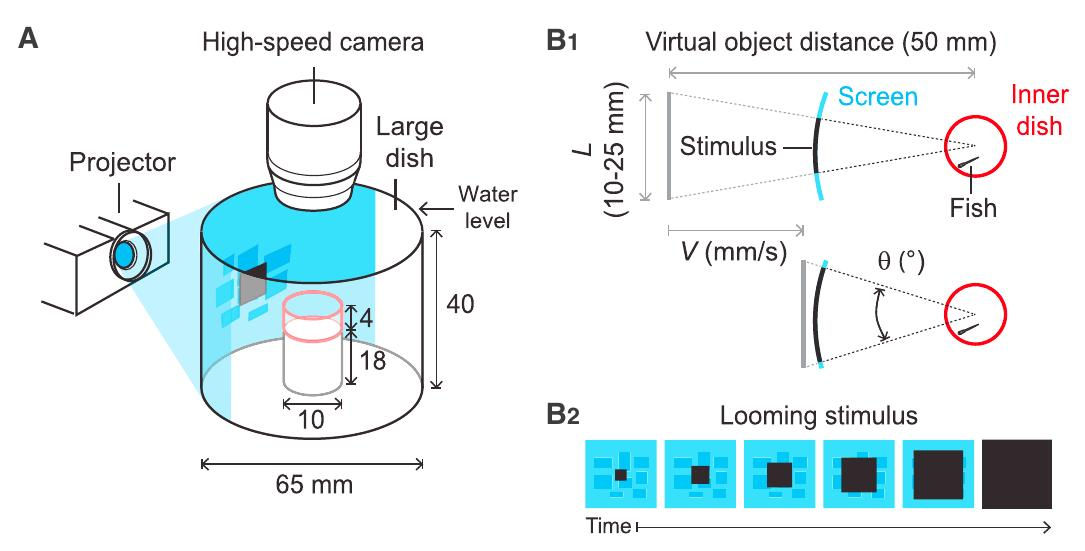
\includegraphics[width=0.8\textwidth]{bhattacharyya_exp_setup.jpeg}
    	\end{center}
    	\caption{\textbf{Experimental setup and stimulus from \cite{Bhattacharyya2017}}. The fish is placed in an inner dish which is located in an larger dish. The stimulus is projected on the wall of the larger dish and the reaction of the fish is recorded from above. Adapted from Figure 1 in \cite{Bhattacharyya2017}.}
    	\label{fig:expm_setup}
    \end{figure}
	For an overview of all reported conditions in the experiments see Table \ref{tab:looming_exp}.\\
	\begin{table} [!th]
		\begin{center}
			\begin{tabular}{l|c|c|c|c}
				%\hline
				\textbf{Study} & \textbf{1} & \textbf{2} & \textbf{3} & \textbf{4}\\
				\hline
				\textbf{Species} & Zebrafish & Zebrafish & Zebrafish & Goldfish\\
				%\hline
				\textbf{Age} & 6-8 dpf & 5-6 dpf & 5 - 7 dpf & -\\
				%\hline
				\textbf{Water temperature [\textdegree C]} & 28  & - & 24  & 18 \\
				%\hline
				\textbf{Screen spanning} & 62 & >100* & >70* & -\\
				\textbf{angle horizontal [\textdegree]} & & & & \\
				%\hline
				\textbf{Screen spanning} & 50 & - & - & -\\
				\textbf{angle vertical [\textdegree]} & & & & \\
				%\hline
				\textbf{Screen distance [cm]} & 1 & - & 3.25 & 16\\
				%\hline
				\textbf{Luminance dark} & 0.07 cd/$m^2$ & 0.7 lux & - & 70-80 lux\\
				%\hline
				\textbf{Luminance grey} & - & 75 lux & - & -\\
				%\hline
				\textbf{Luminance white} & 122.5 cd/$m^2$ & 512 lux & 500 lumen & 300-320 lux\\
				%\hline
				\textbf{L/V values [ms]} & 60-300 \dag & 510 - 2900 \dag & 100 - 
				1200 & 20 - 110*\\
				%\hline
				\textbf{Durations [s]} & 1.65 - 8 & 0.5 - 5* & 1 - 5.5* & 0.25 - 0.8*\\
				%\hline
				\textbf{Acclimation time [min]} & - & - & 15 & -\\
				%\hline
				\textbf{Visual angles [\textdegree]} & 2 - 48 & 25 - 100* & 8 - 70* & 2 - 100*\\
				%\hline
				\textbf{Critical angle [\textdegree]} & 21.7 $\pm$ 2.5 & 72 $\pm$ 1.3 & 35 $\pm$ 15 
				& -\\
				%\hline
				\textbf{Response probabilities} & 20 - 75* & 46 - 60 & 25 - 75* & 70 - 91\\
				%\hline
				\textbf{Head-restrained} & Yes & No & No & No\\
				%\hline
				\textbf{Stimulus shape} & Circle & Circle & Rectangle & Circle\\
				%\hline
				\textbf{Stimulus color} & Black/White, & Black/Chkb. & Black & Black\\
				%\hline
				\textbf{Background color} & White/Black, & Grey & Blue & White\\
				%\hline
				\textbf{Stimulus sizes [cm]} & 0.03 & ? & 1 - 2.5 & 0.5 - 5*\\
				%\hline
				\textbf{Stimulus velocities [cm/s]} & 0.2 - 1 & ? & ? & 20 - 60\\
				%\hline
				\textbf{Initial distances} & ? & ? & 5 & ?\\
				\textbf{(virtual) [cm]} &  &  &  & \\
				%\hline
				\textbf{Projection site} & Side/Front & Bottom & Side/Front & Above\\
				%\hline
			\end{tabular}
		\end{center}
		\caption{The corresponding references of the studies are 1: \cite{Temizer2015}, 
		2: \cite{Dunn2016}, 3: \cite{Bhattacharyya2017} and 4: \cite{Preuss2006}.
		Note that the studies might have conducted other looming stimulus experiments with 
		simultaneous neural recordings but they are not included here because this project is 
		restricted to the behavioral aspects.
		For values denoted with a "\dag" we used the diameter 
		instead of the radius, as it was done in the original studies.
		Values with an "*" are either 
		read of figures or inferred from other, reported values. Chkb. = Checkerboard pattern.}
		\label{tab:looming_exp}
	\end{table}
	%TODO: make appropriate groups for table and/or remove some of them and put the full table into appendix
	For the results of the experiment the time from onset of the stimulus (latency), the distance and the 
	visual angle are measured at the time when the fish responds, i.e. starts to move away.
	The visual angle at response time (response angle) has been found to have the same mean value 
	at different stimulus sizes and velocities in all studies that were done with zebrafish, 
	although there are substantial differences in the mean value as well as in the variance.
	This could be explained by the differences in various experimental conditions such as the water 
	temperature, head restraining or the acclimation time (see Table \ref{tab:looming_exp}).
	While the study with goldfish \citep{Preuss2006} does not report to find a so-called critical visual angle, the observed response angles (14\textdegree{} to 29\textdegree) are in a range 
  	that is comparable to e.g. the one found by \cite{Bhattacharyya2017} (35\textdegree{} $\pm$ 
	15\textdegree).
    The distribution of response angles in dependence of the L/V values of all studies considered here is shown in Figure \ref{fig:expm_theta_lv}.\\
    \begin{figure}[!h]
    	\begin{center}
			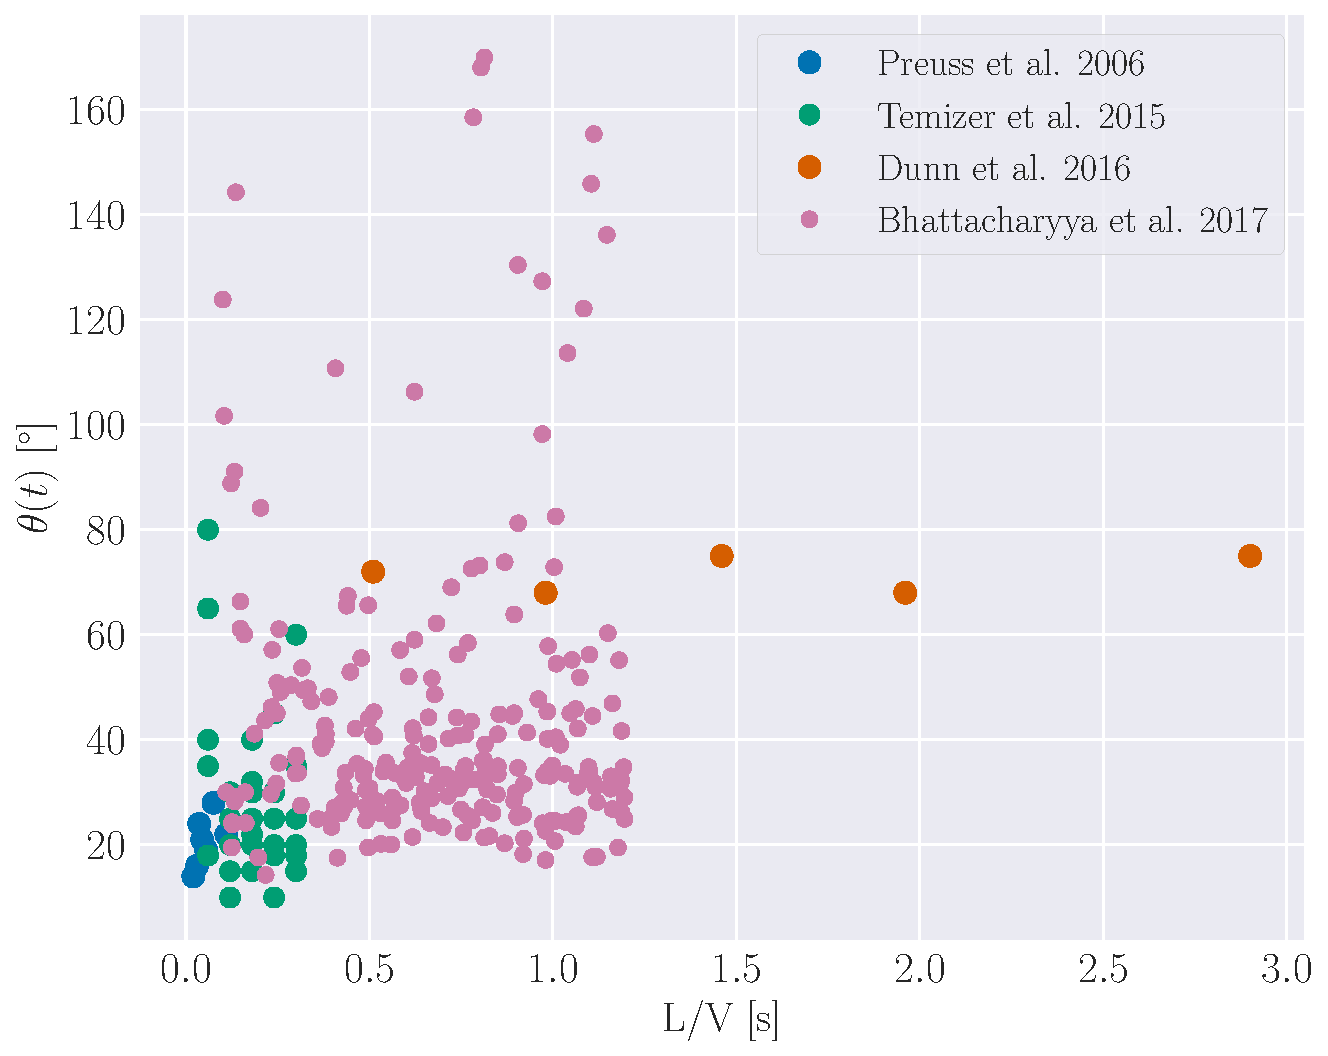
\includegraphics[width=0.8\textwidth]{figure_expm_theta_vs_lv.pdf}
    	\end{center}
    	\caption{Experimental response angles against L/V values.}
    	\label{fig:expm_theta_lv}
    \end{figure}
	For the simulations of the experiment we closely followed the procedure reported by 
	\cite{Bhattacharyya2017}.
	At the beginning of a trial a stimulus size is drawn from a uniform distribution between 10 mm and 25 mm.
	Next, an L/V value is uniformly drawn between 0.1 s and 1.2 s and the resulting velocity for the 
	trial stimulus size is calculated.
	With the trial stimulus size $L_{trial}$ and the trial velocity $v_{trial}$ the visual angle 
	over time $\theta(t)$ is calculated by:
	\begin{equation}
	\theta (t) = 2\cdot \arctan(\frac{L_{trial}/2}{D_{init} - v_{trial}\cdot t}),
	\label{eq:theta}
	\end{equation}
	where $D_{init}$ is the virtual initial distance which is set to 50mm if not stated otherwise.
    The range of possible time courses of the visual angle is shown in Figure \ref{fig:theta_lv} A.
    Note that because the initial distance is fixed and we sample from different stimulus sizes we get different initial angles for the same L/V values.
    This leads to different time courses for the same L/V value depending on the stimulus size but starting from the same angle their time courses are identical (Figure \ref{fig:theta_lv} B).
    If we now assume a critical angle $\theta_{crt}$ at which the fish escapes, we can describe how the response time, response distance and time-to-collision (TTC) at response depend on the L/V value.
    The response time linearly depends on the L/V while the slope of the relationship is determined by stimulus size $L$, initial distance $D_{init}$ and critical angle $\theta_{crt}$:
	\begin{equation}
	t_{resp} = \dfrac{L}{v} \left(\dfrac{D_{init}}{L} - \dfrac{1}{2\cdot\tan(\theta_{crt} /2)}\right).
	\label{eq:resp_time}
	\end{equation}
    The response distance only depends on the stimulus size $L$:
    \begin{equation}
	D_{resp} = \dfrac{L}{2\cdot \tan(\theta_{crt} /2)}.
	\label{eq:resp_dist}
	\end{equation}
    The TTC linearly depends on $L/V$ and the slope is determined only by the critical angle $\theta_{crt}$:
	\begin{equation}
	TTC_{resp} = - \dfrac{L}{2\cdot v\cdot \tan(\theta_{crt} /2)}.
	\label{eq:resp_ttc}
	\end{equation}
    For an example with $\theta_{crt}=35$ and $D_{init}=50$ these idealized response properties are illustrated in Figure \ref{fig:ideal_resp_props}, where we chose the same axes as in Figure 1 of \cite{Bhattacharyya2017} for easy comparison.\\
	In our simulations the visual angle is next transformed by a linear function and the result is the input $I(t)$ for our neuronal model, described in the previous chapter:
	\begin{equation}
	I(t) = f(\theta (t)) = c_{scale}(m \cdot \theta(t) + b).
	\label{eq:input}
	\end{equation}
	In order to calculate the response properties we take the time of the first spike $t_{spk}$ of the model M-cell after stimulus onset as the response time of the fish.
	We ignore further processing time after the spike because it is in the order of milliseconds \citep{Preuss2003} and thus irrelevant with respect to the overall response time which is in the order of at least hundreds of milliseconds for visual stimuli \citep{Preuss2006}.
	Thus the response angle of the simulated trial will be $\theta (t_{spk})$.
	%TODO: mention initial period with constant size
	
    \begin{figure}[H]
    	\begin{center}
			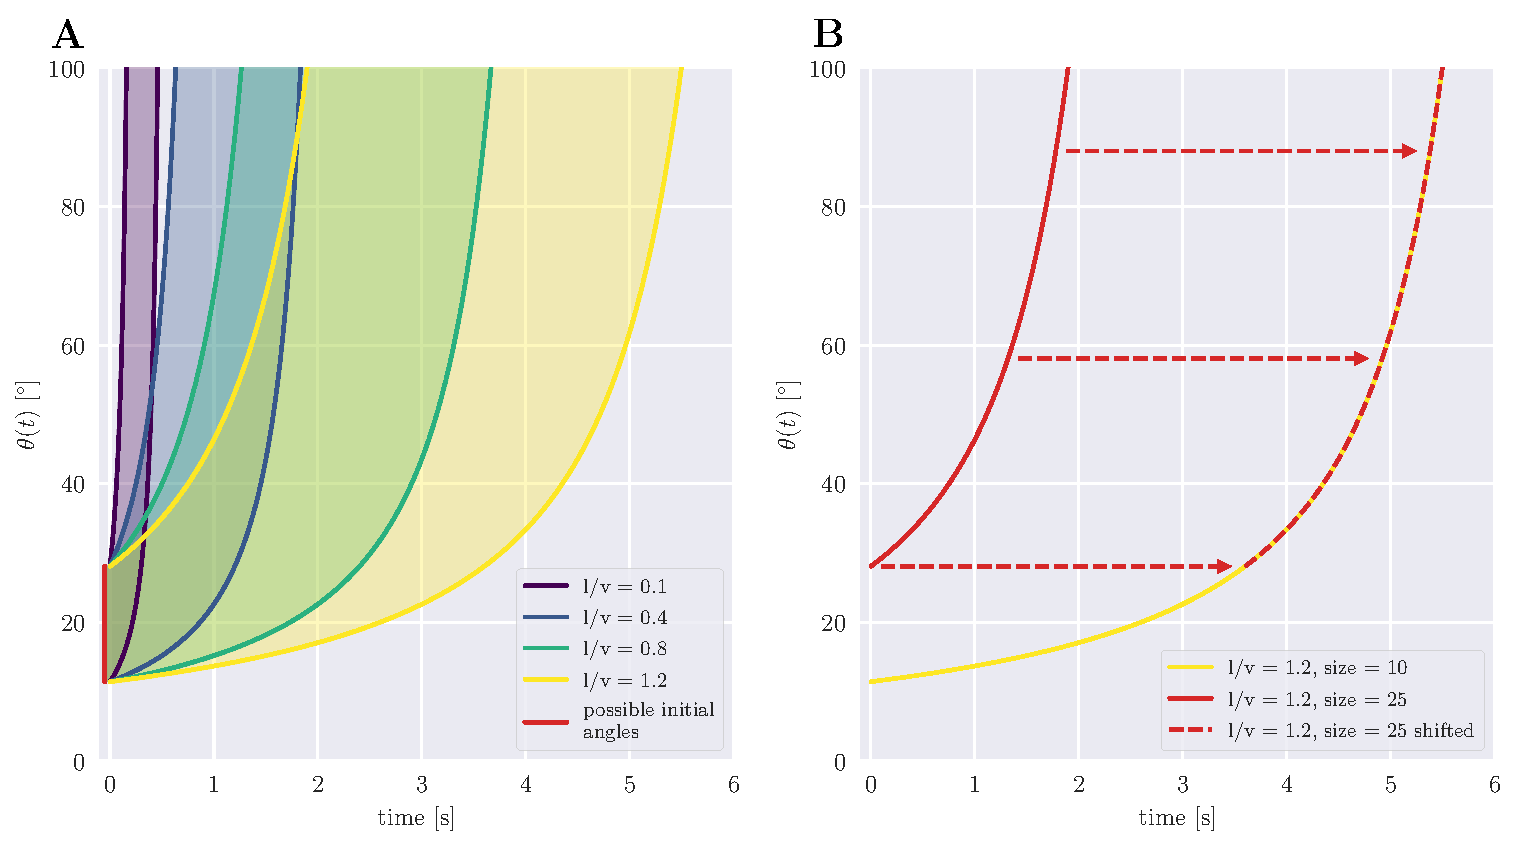
\includegraphics[width=\textwidth]{figure_theta_lv_test.pdf}
    	\end{center}
    	\caption{Range of time courses of $\theta$ depending on L/V. \textbf{A} For four different L/V values the possible time courses are shown if stimulus size L ranges between 10 mm and 25 mm. \textbf{B} Single time courses for the same L/V value only differ in a horizontal shift that is introduced by the different initial angle.}
    	\label{fig:theta_lv}
    \end{figure}
    
    \begin{figure}[H]
    	\begin{center}
			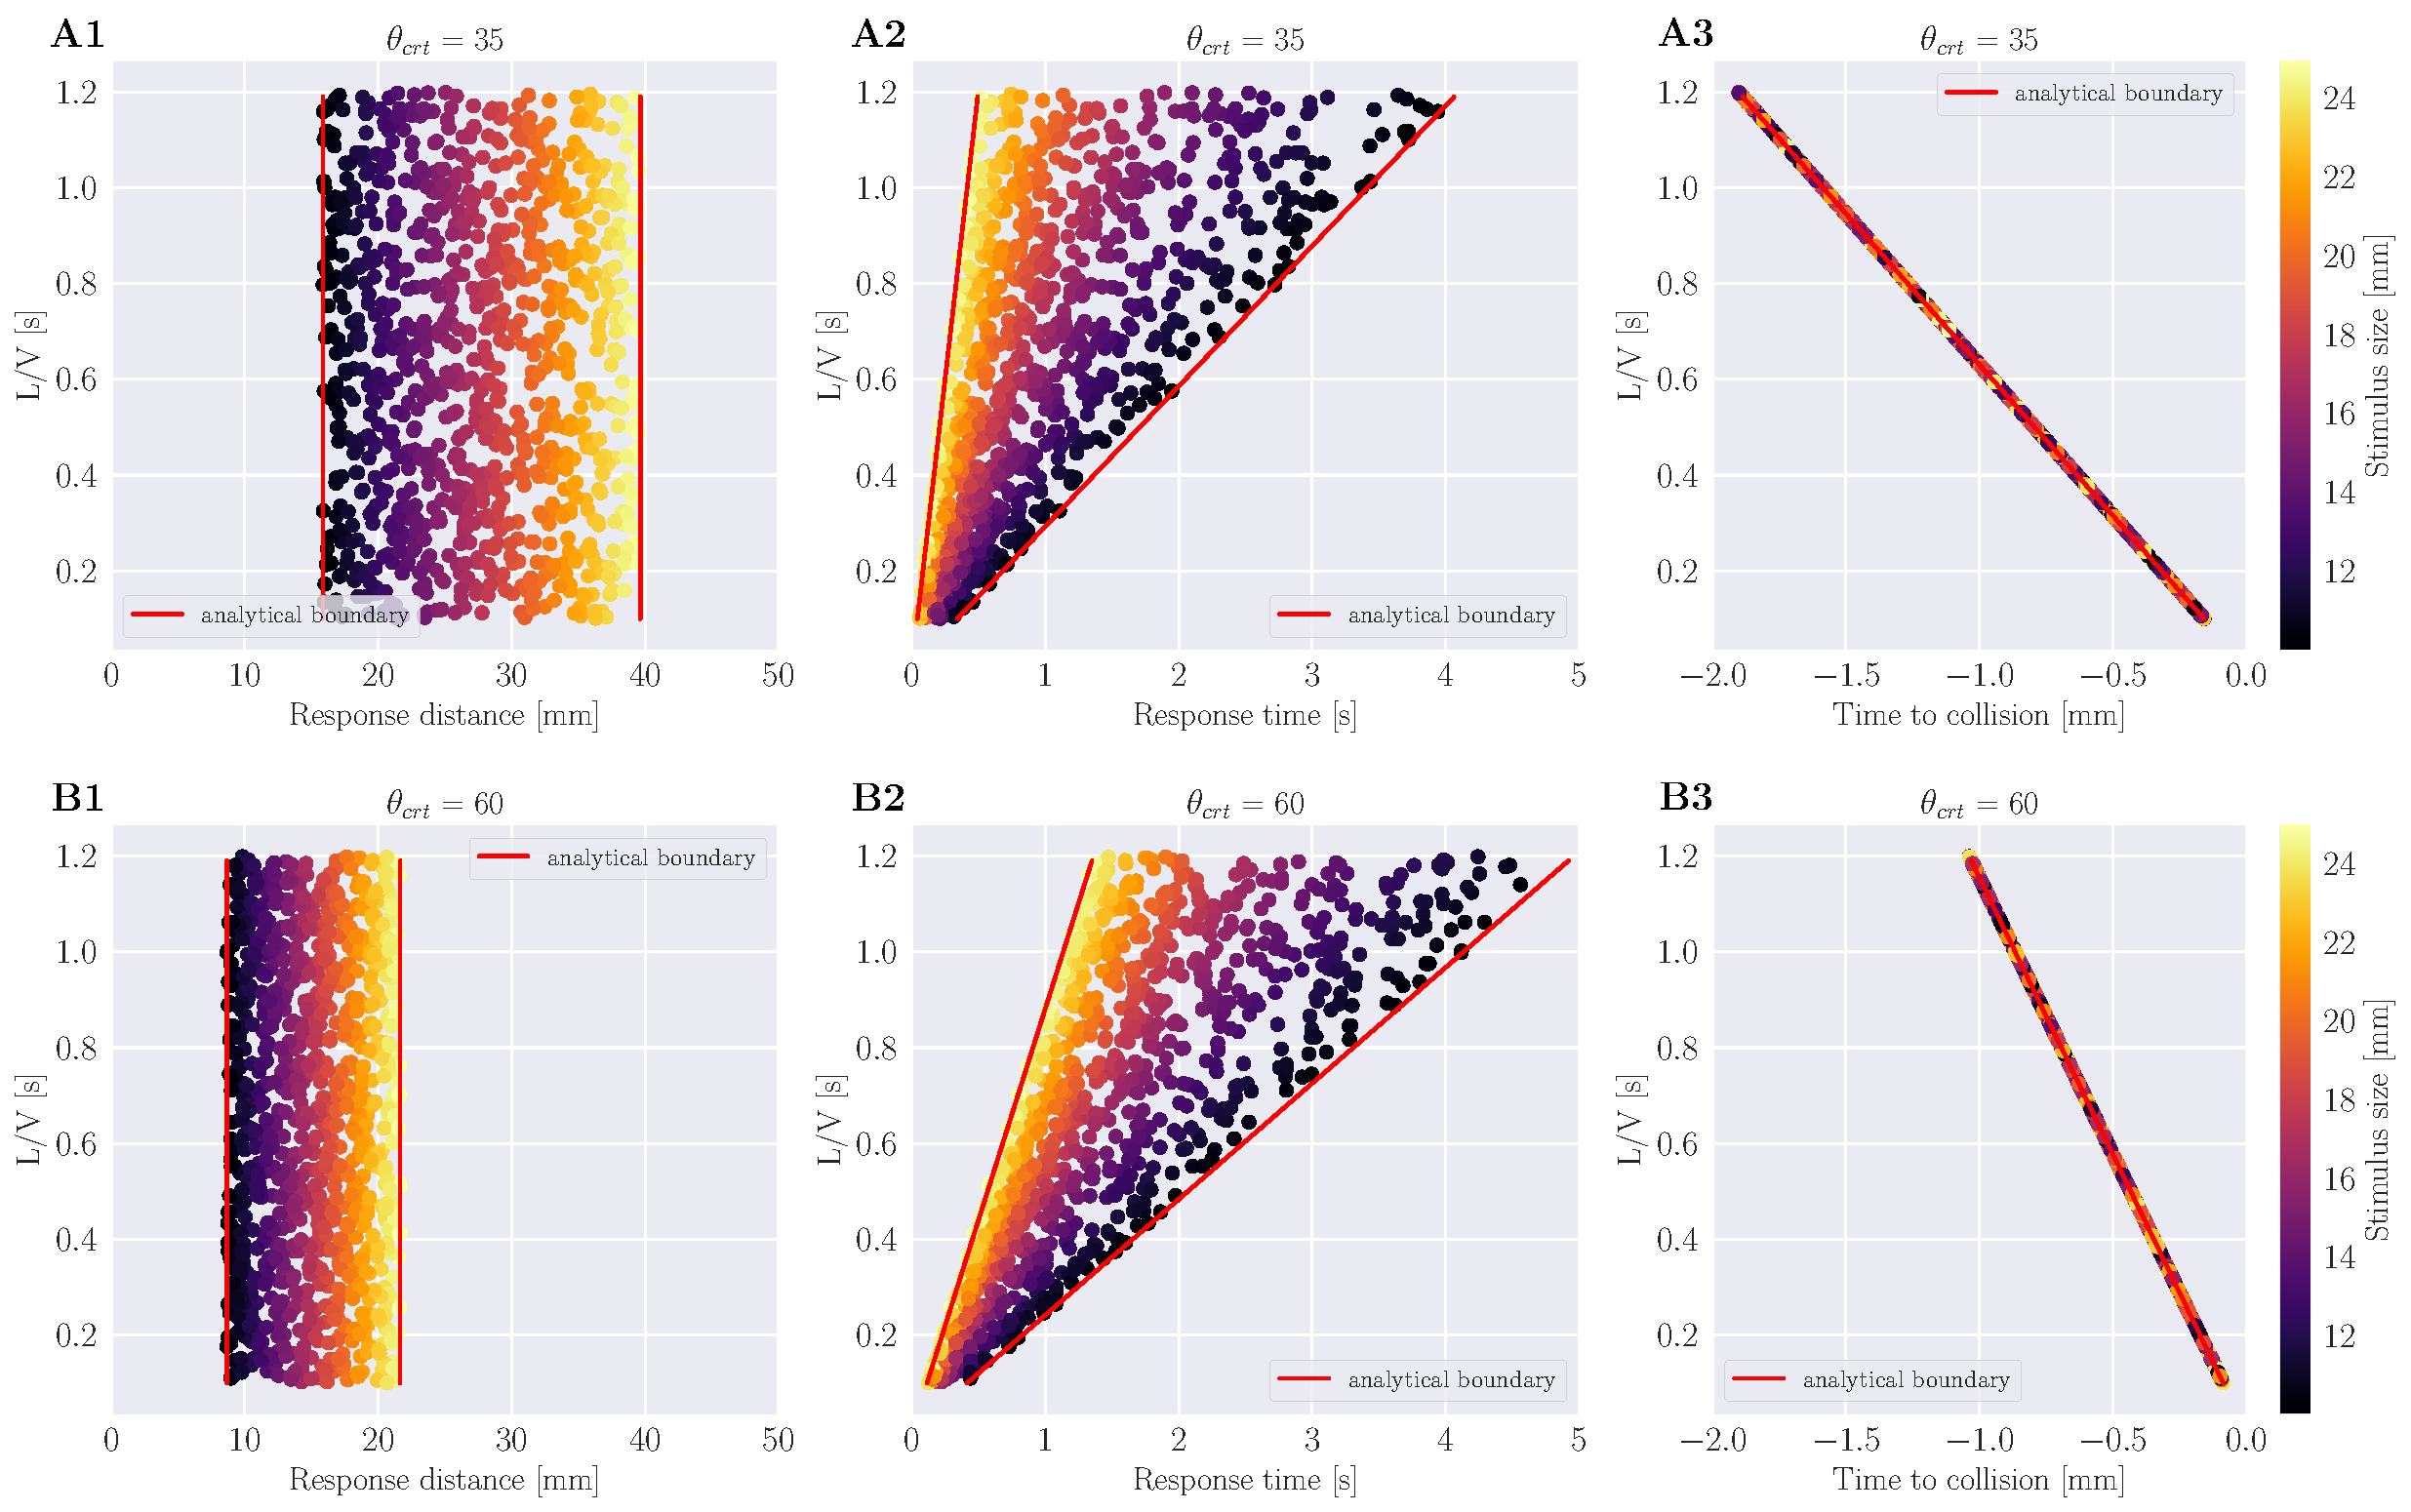
\includegraphics[width=\textwidth]{figure_ideal_resp_v2.pdf}
    	\end{center}
    	\caption{Response properties for a critical angle $\theta_{crt}=35$ and initial distance $D_{init}=50$ mm.  For all plots L was sampled between 10 mm and 25 mm and L/V was sampled between 0.1 s and 1.2 s. Red lines show minimal and maximal values that were calculated using equations \ref{eq:resp_time}, \ref{eq:resp_dist} and \ref{eq:resp_ttc}. \textbf{A} The response distance only depends on L and thus has the same range for all L/V values. \textbf{B} Response times linearly increase with L/V and the slope increases for smaller L. \textbf{C} Absolute time-to-collision linearly increases with L/V and the slope only depends on $\theta_{crt}$.}
    	\label{fig:ideal_resp_props}
    \end{figure}
		
	\section{Stationary Approximation of Full Model}
    For the stationary approximation of the full model in section \ref{approx full model} we derived an analytical solution for the input at which the M-cell fires if there is no noise in the system (see equation \ref{eq:crit_input}).
    Since we defined the time of the first spike of the M-cell as the time at which the fish responds this approximated model therefore has a deterministic response angle.
    Using our definition of the input in the visual looming stimulus experiment from equation \ref{eq:input} we find the following expression for the response angle:
    \begin{equation}
	I(t) = f(\theta(t)) \overset{!}{=} \frac{V_t - E_{L} + \rho_{0}}{(R_{m} - c_{\rho})}
	\label{eq:crit_theta_start}
	\end{equation}
    \begin{equation}
	\Leftrightarrow \theta \overset{!}{=} \frac{V_t - E_{L} + \rho_{0}}{c_{scale}\cdot m \cdot (R_{m} - c_{\rho})} - \frac{b}{m}
	\label{eq:crit_theta_end}
	\end{equation}
	Because we fix the parameters $E_{L}=-79$ mV, $R_{m}=10$ M$\Omega$ and $V_{t}=-61$ mV, the remaining free parameters for this model are $\rho_{0}$, $c_{\rho}$, $c_{scale}$, $m$ and $b$.
    The response angle linearly increases with $\rho_{0}$ and linearly decreases with $b$.
    The influence of $b$ is scaled by $m$ and for $\rho_{0}$ the increase is scaled by the product of $(R_{m} - c_{\rho})$, $c_{scale}$ and $m$.
    Furthermore, the response angle is reversely proportional to $c_{scale}$ and $m$.
    If $c_{\rho} > R_{m}$ the model predicts a negative response angle because this would mean that the effective input for the M-cell is negative.
    As this is unrealistic we constraint $c_{\rho}$ to be strictly smaller than $R_{m}$.
    For the allowed range the response angle increases with increasing $c_{\rho}$ and the increases become larger as $c_{\rho}$ approaches $R_{m}$.
    For a simplified case where we fix $b=0$ and $c_{scale}=3\cdot10^{-10}$, the effect of the remaining free parameters on the response angle is shown in Figure \ref{fig:effect_stationary_params}.\\
    If we now look at the effects of adding noise to the system, first we have to specify the random distribution for the resting activity of the inhibitory population $\rho_0$.
    Motivated by the rarely occurring but very high response angles in the data of \cite{Bhattacharyya2017} (see Figure \ref{fig:expm_theta_lv}) we chose the log-normal distribution that is parametrized by the mean $\mu_{\rho_{0}}$ and the standard deviation $\sigma_{\rho_{0}}$ of the normal distribution it is derived from:
    \begin{equation}
	 ln(P_{0}) \sim \mathcal{N}(\mu_{\rho_{0}},\,\sigma_{\rho_{0}}^{2}).
	\label{eq:rho_null}
	\end{equation}
    The main difference from a normal distribution is that the log-normal distribution has much higher probabilities for high values, also called a "fat tail" and this will allow the model to account for the rare but high response angles.\\
    For the stationary model, all sources of noise that we consider here: membrane potential, firing threshold, inhibitory population activity and the resting activity of the inhibitory population, all have qualitatively the same linear effect on the response angle that is exemplified by the effect of $\rho_0$ in Figure \ref{fig:effect_stationary_params} C.
    This means that the distribution of response angles will closely follow the noise distribution.
    For the Gaussian noise on the membrane potential the response angles are approximately normally distributed and the mean and variance of the distribution depend on the variance of the added noise.
    The mean response angle decreases with increasing variance and the variance of the distribution increases with increasing variance of the noise (Figure \ref{fig:effect_noise_stationary} A1 and B1).
    Combining two sources of noise increases these effects (Figure \ref{fig:effect_noise_stationary} A2 and B2).\\
    Note, that the decrease of the mean response angle is due to the noise being instantaneous in our case, which effectively models fast threshold fluctuations with extremely short relaxation times.
    If we look at noise on the threshold for an example, this means that at each point in time, there is a high probability that the threshold is much lower than its average value which effectively lowers the threshold on average.
    If, on the other hand, the threshold was described by a stochastic process with a large relaxation time we could say that the threshold would be constant for the time of a single trial and the value would be a sample from the distribution.
    In Figure \ref{fig:static_vs_dynamic_noise} we compare these two extreme cases and see that for the "constant" noise, the mean value of the response angle distribution does not change (Figure \ref{fig:static_vs_dynamic_noise} B).\\
    For the log-normally distributed noise on the resting activity of the inhibitory population the response angles again follow the noise distribution (Figure \ref{fig:effect_rho_null_stationary}).
    At higher variances there are trials in which the inhibition is so strong that the M-cell does not fire at all within the trial time (bars at 180\textdegree{} in Figure \ref{fig:effect_rho_null_stationary}).
    \begin{figure}[H]
    	\begin{center}
			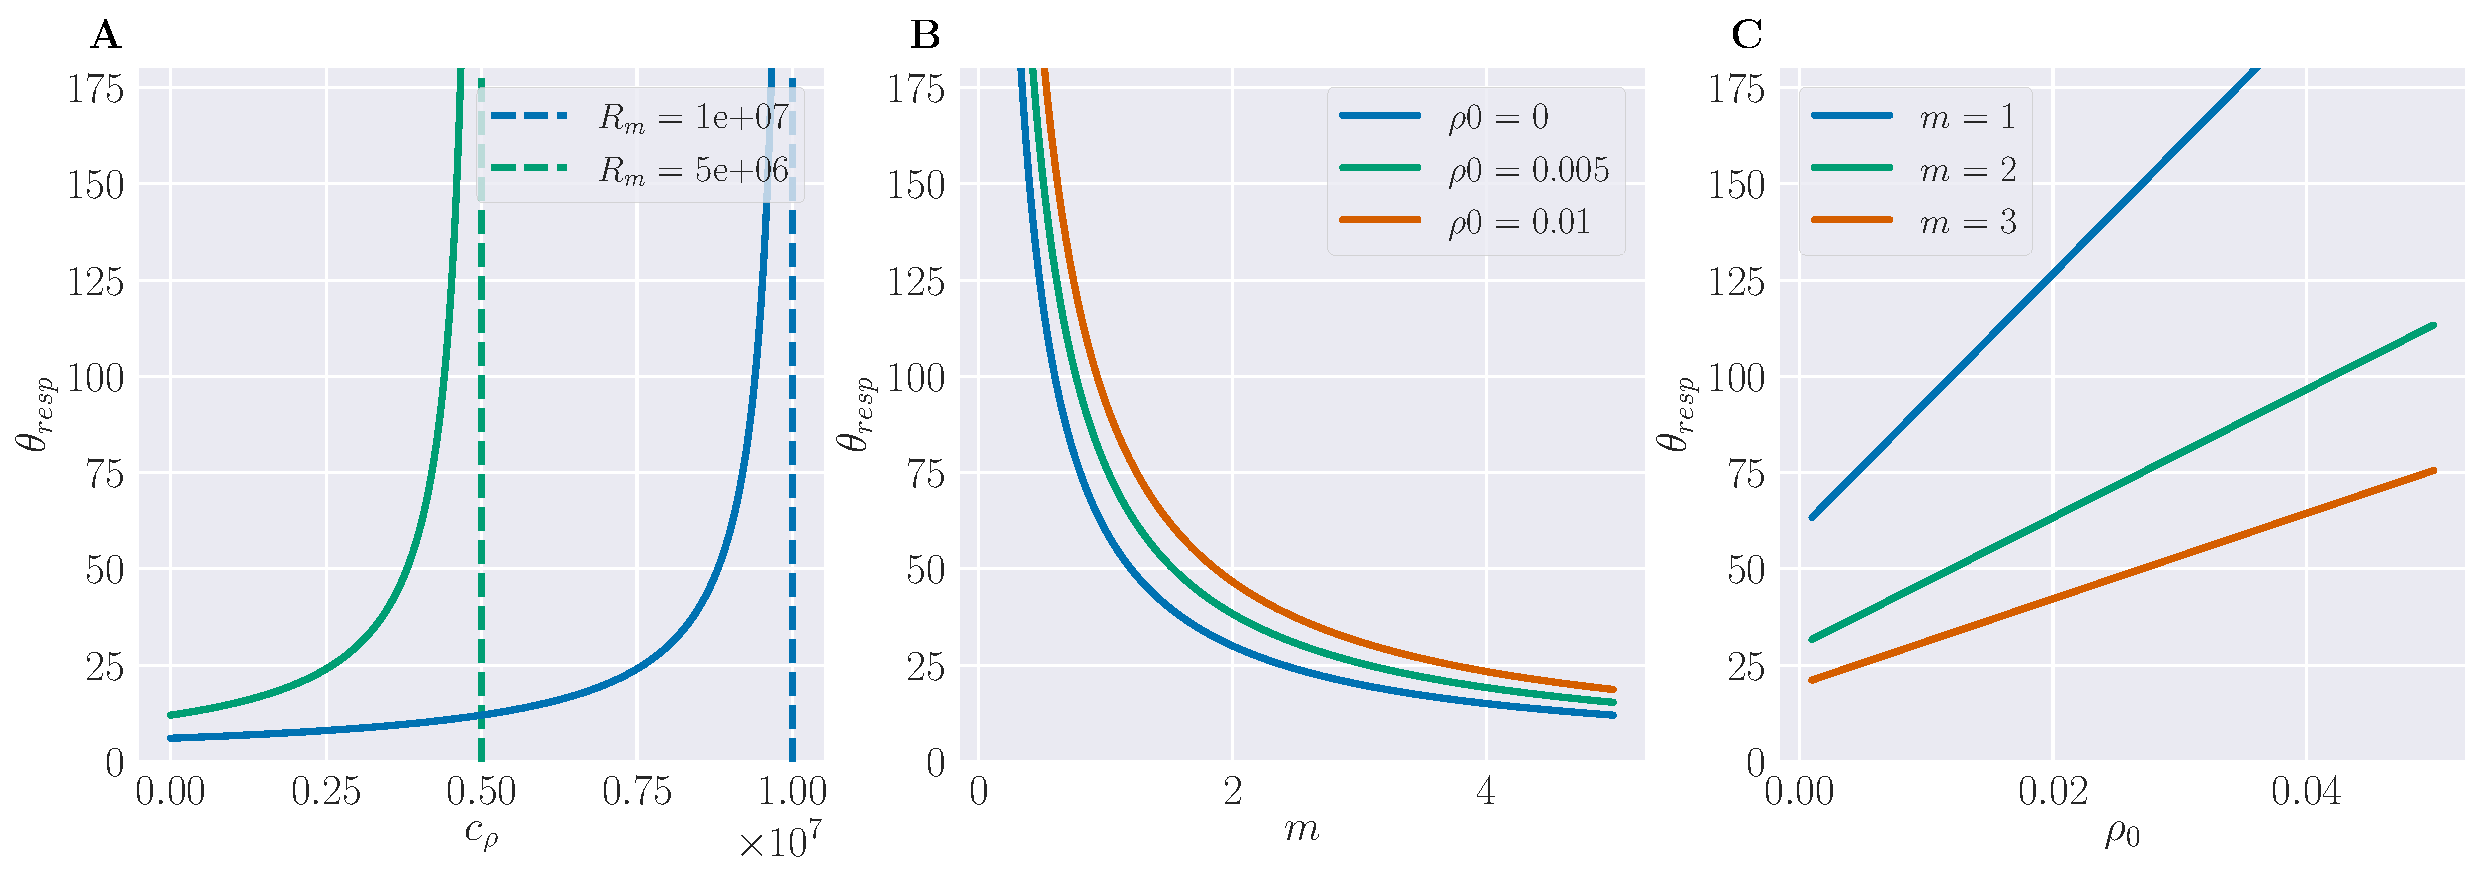
\includegraphics[width=\textwidth]{figure_stationary_params.pdf}
    	\end{center}
    	\caption{\textbf{Effect of parameters on response angle in the noise-free, stationary model.}  For $b=0$ and $c_{scale}=3\cdot10^{-10}$. \textbf{A} Response angle increases exponentially with the scaling of the input for the inhibitory population. For two different values of the membrane resistance $R_{m}$. \textbf{B} Response angle decreases exponentially with the slope of the linear transformation of the visual angle. \textbf{C} Response angle increases linearly with higher resting activity of the inhibitory population.}
    	\label{fig:effect_stationary_params}
    \end{figure}
    
    \begin{figure}[H]
    	\begin{center}
			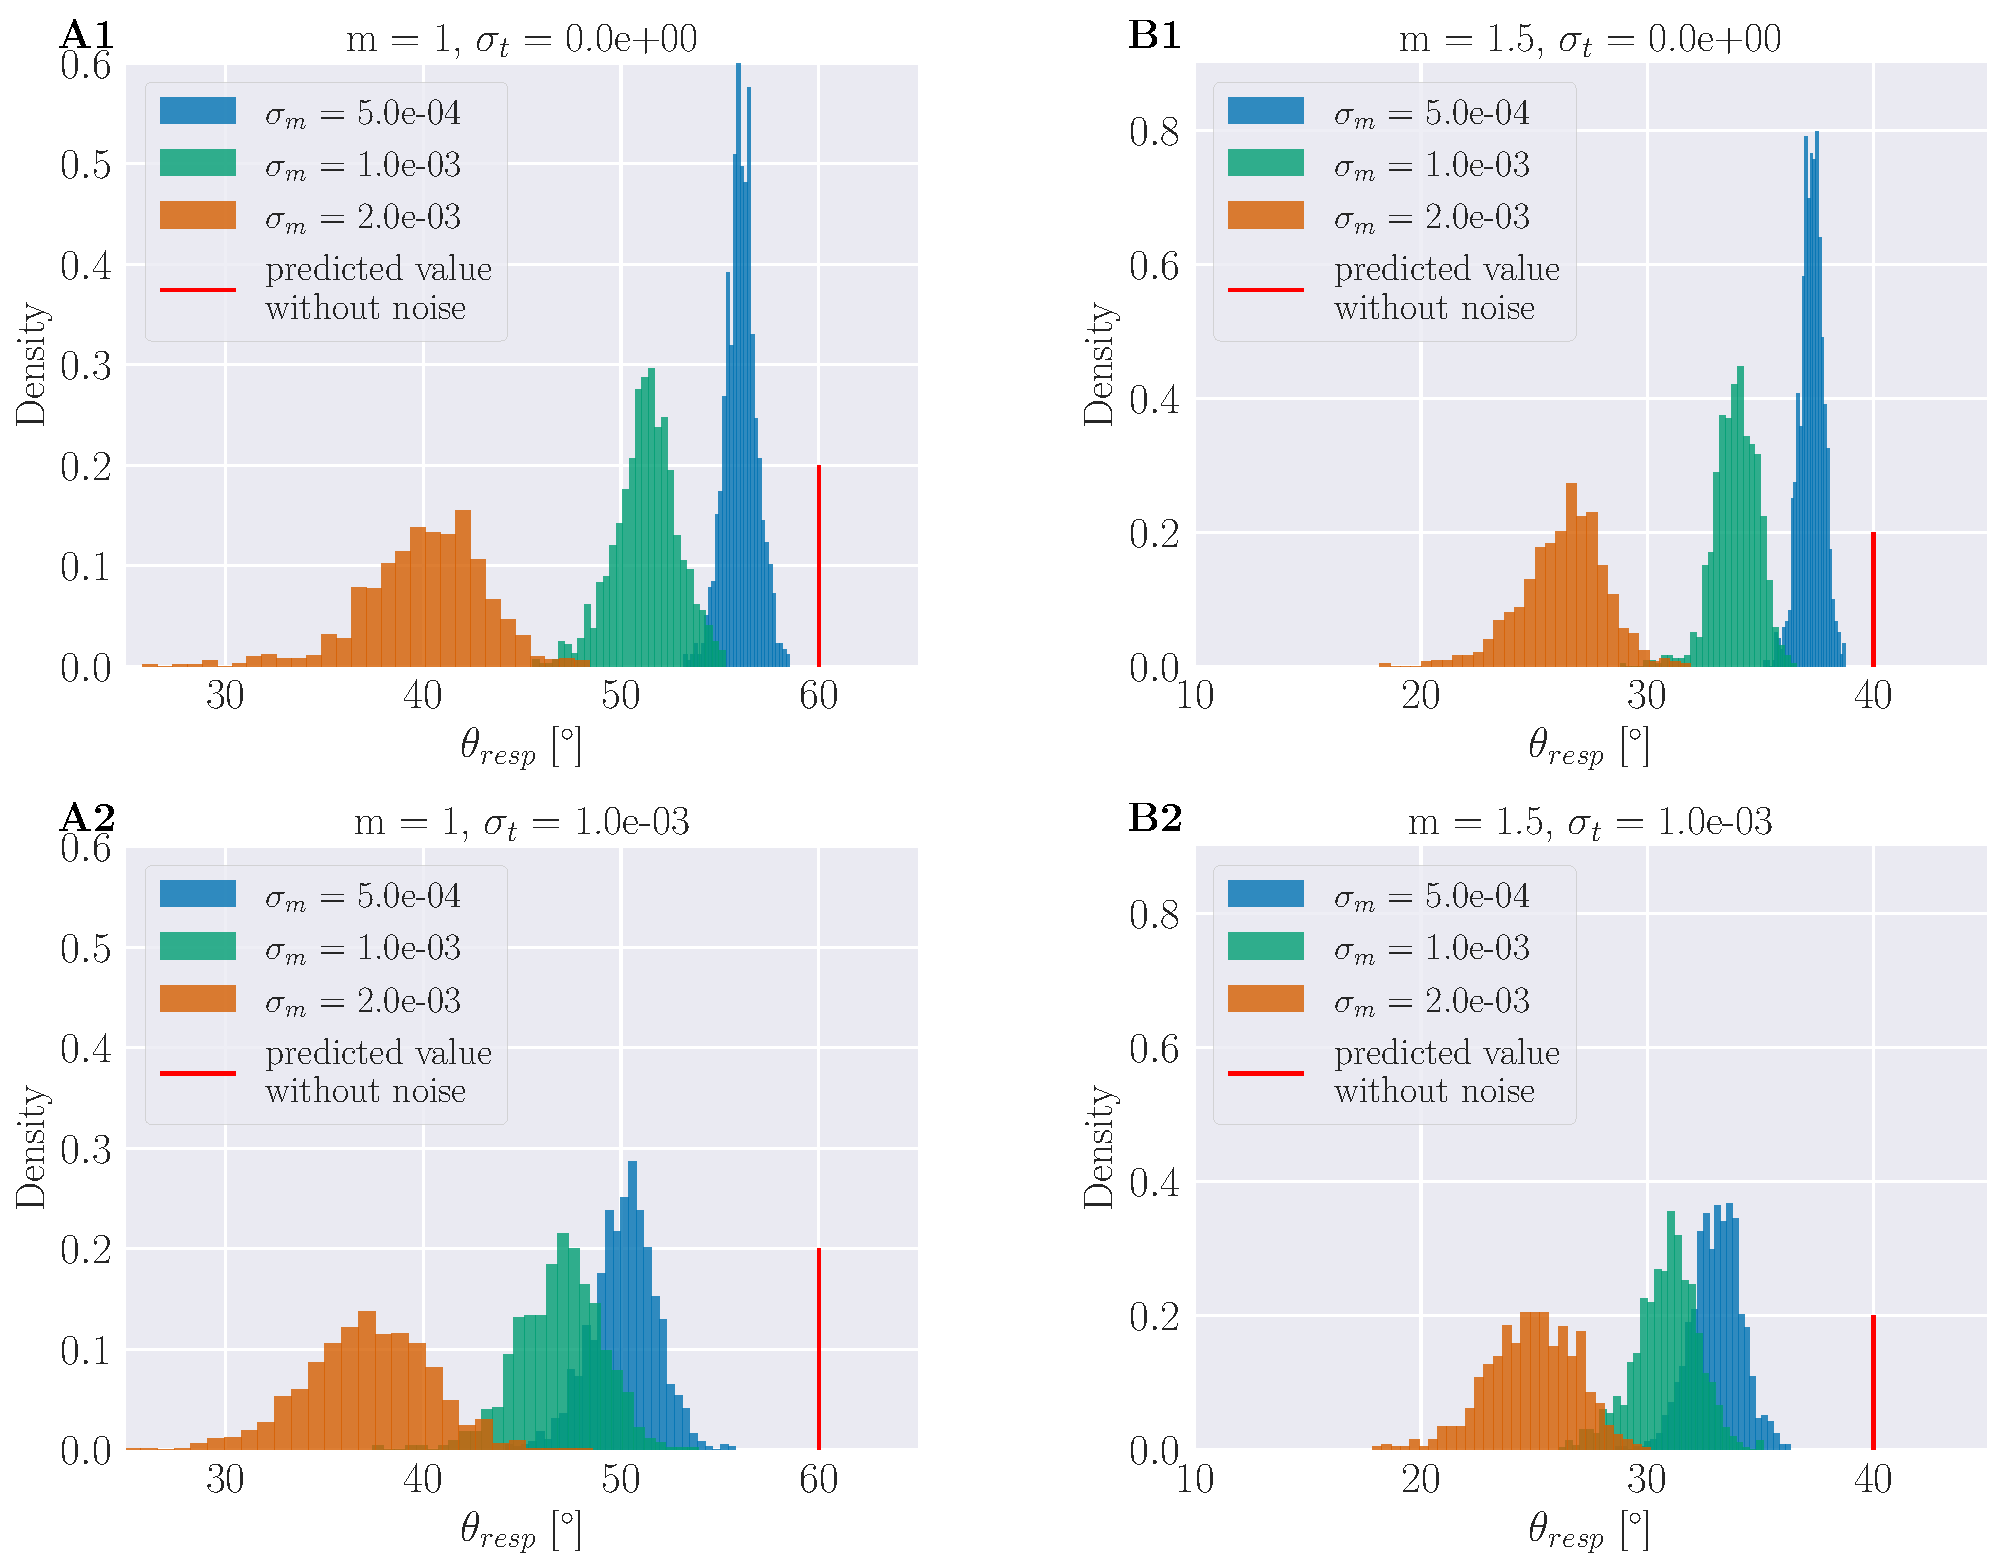
\includegraphics[width=\textwidth]{figure_stationary_noisy_params.pdf}
    	\end{center}
    	\caption{\textbf{Response angle distributions for membrane potential and threshold noise.} For $b=0$, $c_{scale}=3\cdot10^{-10}$, $\rho_{0}=0$, $c_{\rho}=0.9\cdot 10^{7}$. Increasing the variance of the noise decreases the mean response angle and increases the variance of the distribution of response angles. This is independent of the value of the response angle without noise (\textbf{A} vs. \textbf{B}). The effects of two noise sources together add up in a nonlinear way (\textbf{A1} vs. \textbf{A2} and \textbf{B1} vs. \textbf{B2}).}
    	\label{fig:effect_noise_stationary}
    \end{figure}
    
    \begin{figure}[H]
    	\begin{center}
			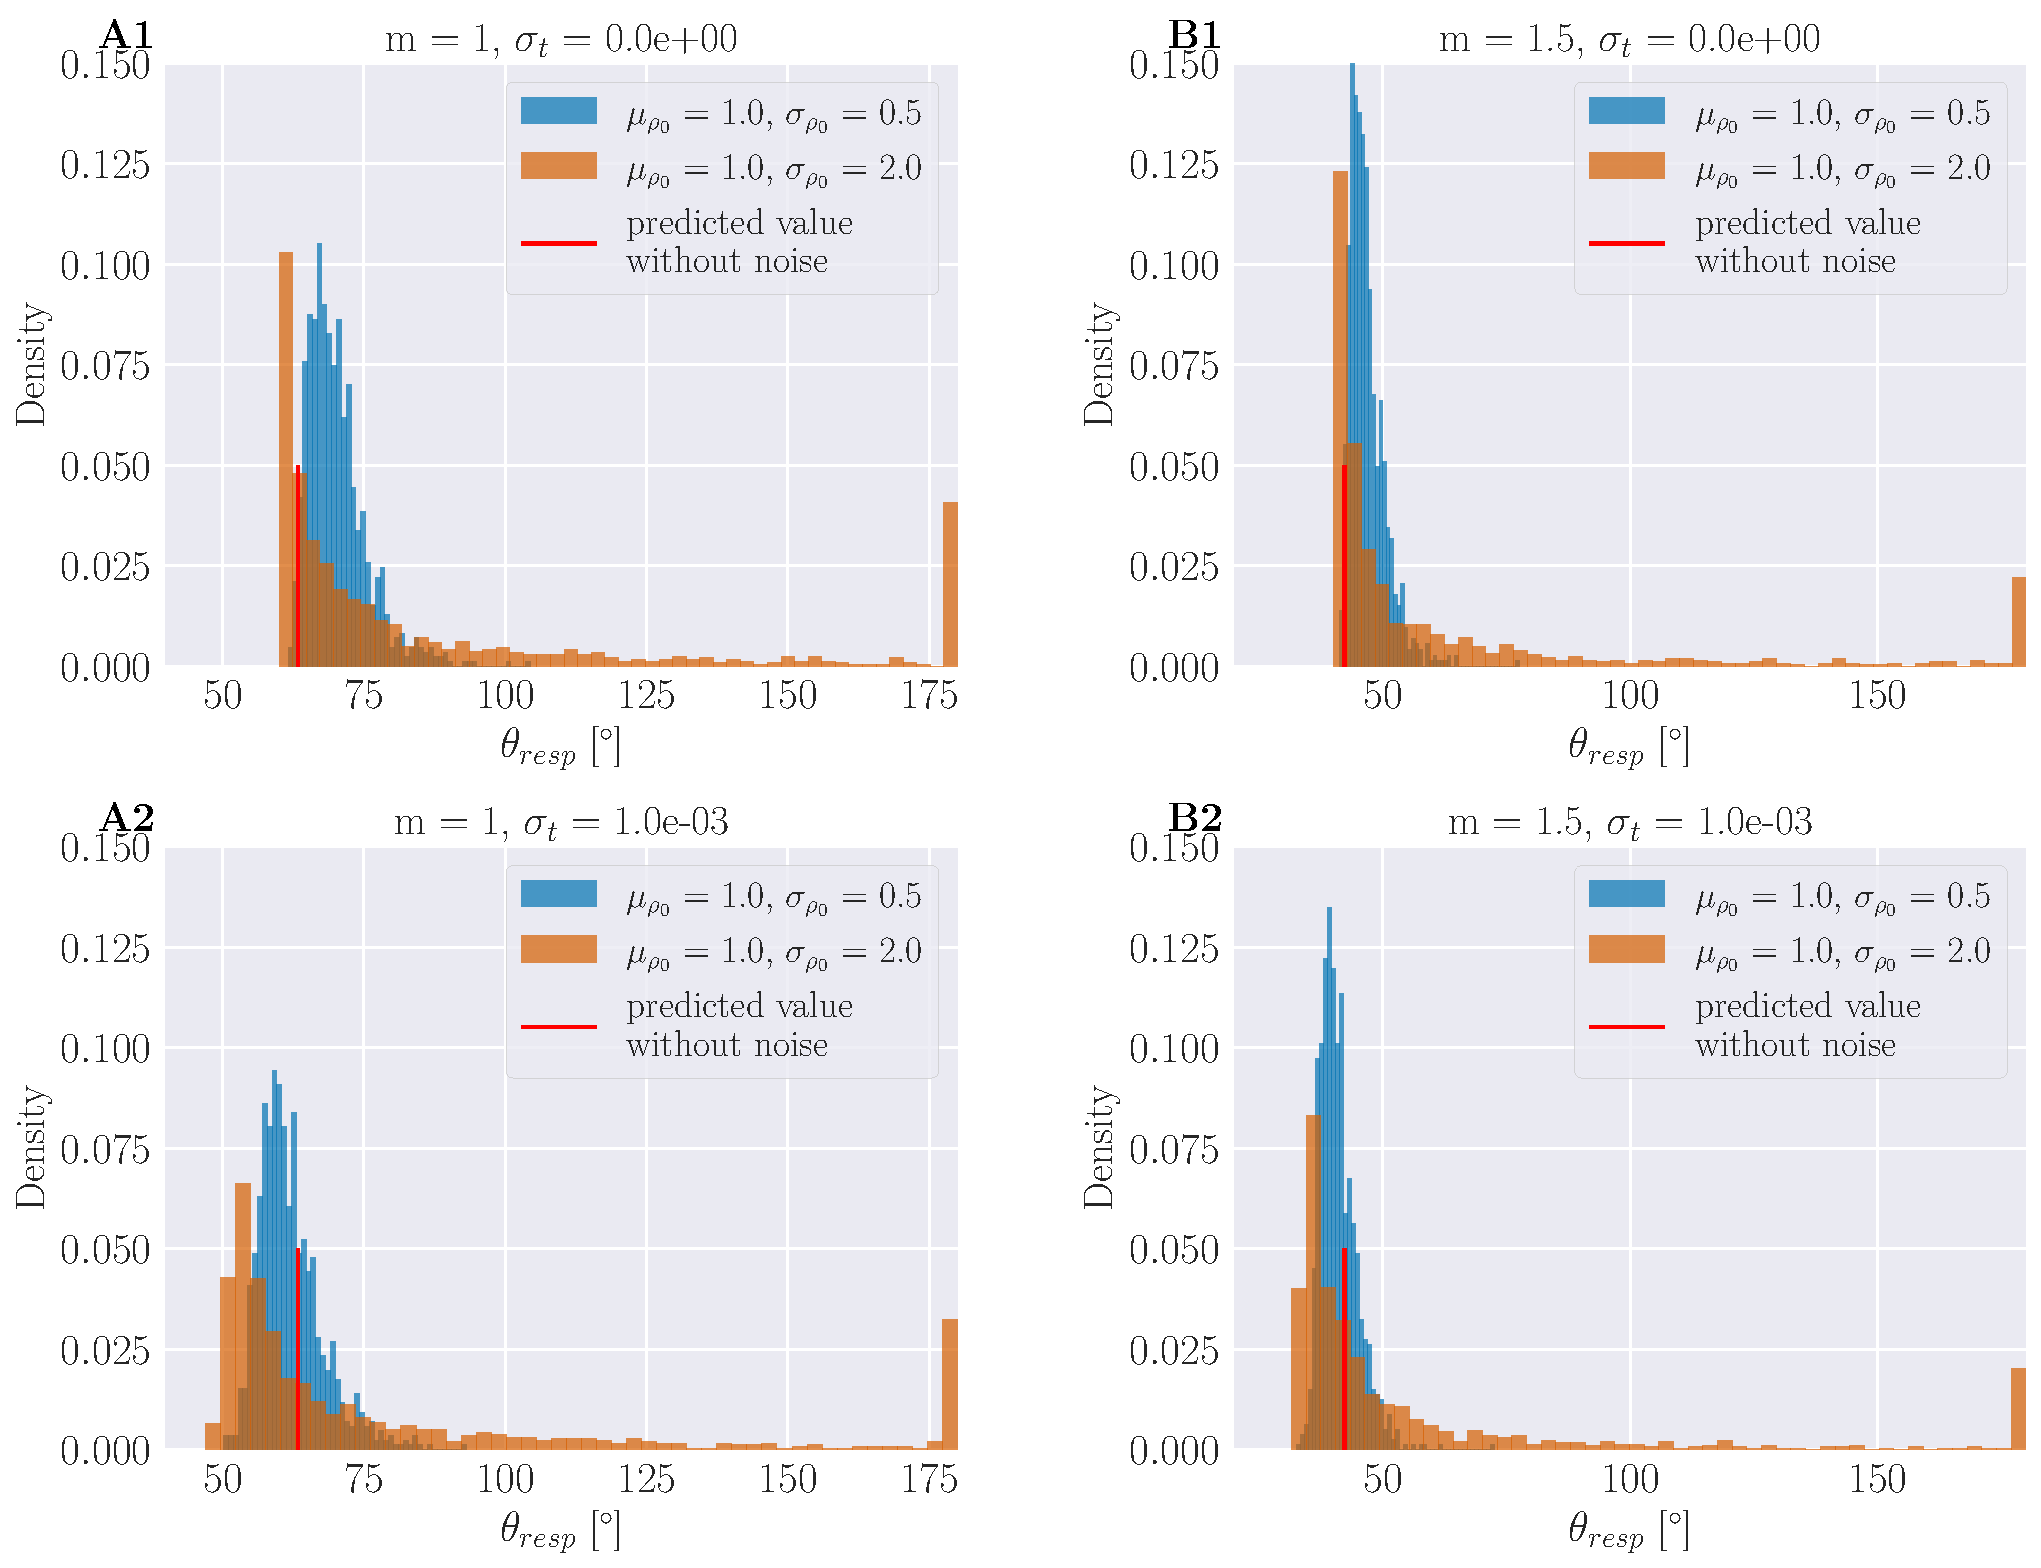
\includegraphics[width=\textwidth]{figure_stationary_rho_null_noise.pdf}
    	\end{center}
    	\caption{\textbf{Response angle distributions for noise of the resting activity of the inhibitory population.} For $b=0$, $c_{scale}=3\cdot10^{-10}$, $c_{\rho}=0.9\cdot 10^{7}$. Sampling the resting activity of the inhibitory population from a log-normal distribution generally increases the response angle. For a small variance the response angle distribution is similar to a Gaussian distribution. Increasing the variance reduces the mode of the distribution but introduces a long tail of higher response angles. The bar at 180 \textdegree{} represents trials for which the M-cell did not fire. These effects are independent of the value of the response angle without noise(\textbf{A} vs. \textbf{B}). Adding threshold noise shifts the distribution towards smaller response angles as observed in Figure \ref{fig:effect_noise_stationary} and minimally changes the shape of the distribution (\textbf{A2} and \textbf{B2}.}
    	\label{fig:effect_rho_null_stationary}
    \end{figure}
    
    \begin{figure}[H]
    	\begin{center}
			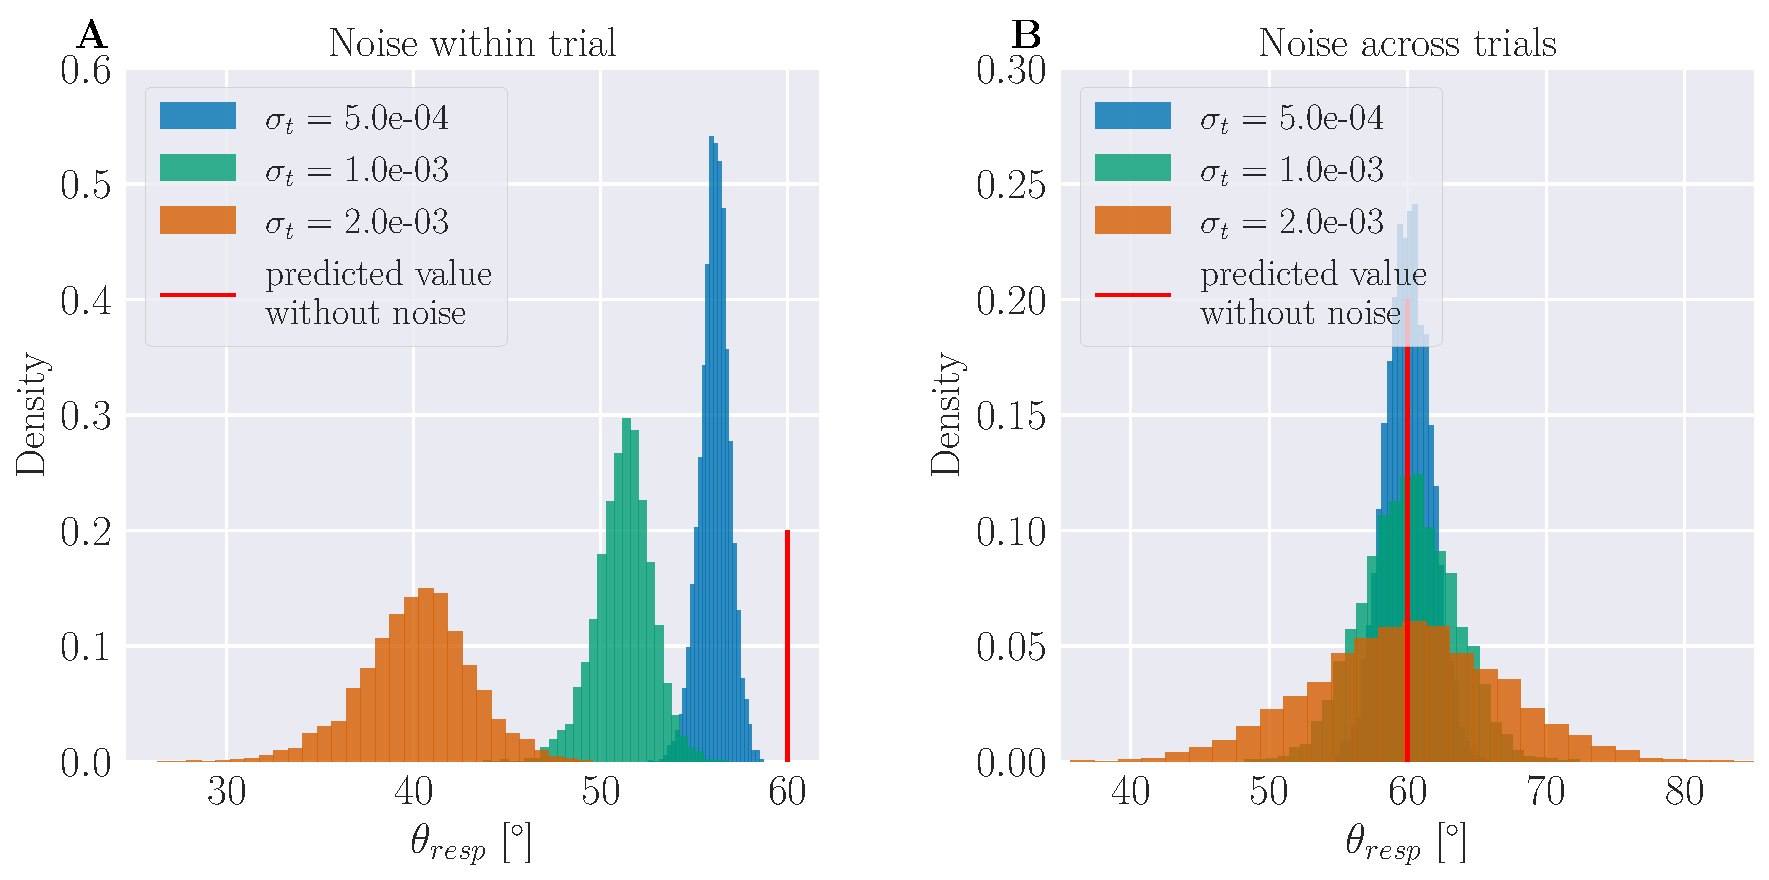
\includegraphics[width=\textwidth, height=0.25\textheight]{figure_static_vs_dynamic_noise.pdf}
    	\end{center}
    	\caption{\textbf{Instantaneous versus constant noise.} While instantaneous noise (\textbf{A}) also decreases the mean response angle, constant noise (\textbf{B}) only affects the variance of the resulting response angle distribution.}
    	\label{fig:static_vs_dynamic_noise}
    \end{figure}

    \section{Stationary approximation of Inhibitory Population}
    In the model of section \ref{approx inhibition}, equation \ref{eq:inhib_approx} we only approximated the activity of the inhibitory population.
    In comparison with the previous section the only difference is that the membrane potential $V_{m}$ now follows the differential equation and thus integrates the input on a time scale that is set by the membrane time constant $\tau_m$ which has been found to be 23 ms in the study of \cite{Koyama2016}.
    For the fastest stimuli (small L/V values) this leads to a deviation from the stationary solution of the previous section (Figure \ref{fig:station_inh_resp_angle}).
    In these cases the response angle is bigger than the response angle predicted by the stationary solution because the input is integrated with a delay so that by the time the membrane potential reaches the threshold, the visual angle already increased beyond the critical value that we would expect from the stationary solution.
    As expected, the deviation increases as the L/V values become smaller (and therefore faster for the same stimulus size).
    The deviation also increases for a bigger $\tau_m$ and decreases for a smaller $\tau_m$, further supporting the notion that the deviation stems from the slower time scale.
        
    \begin{figure}[H]
    	\begin{center}
			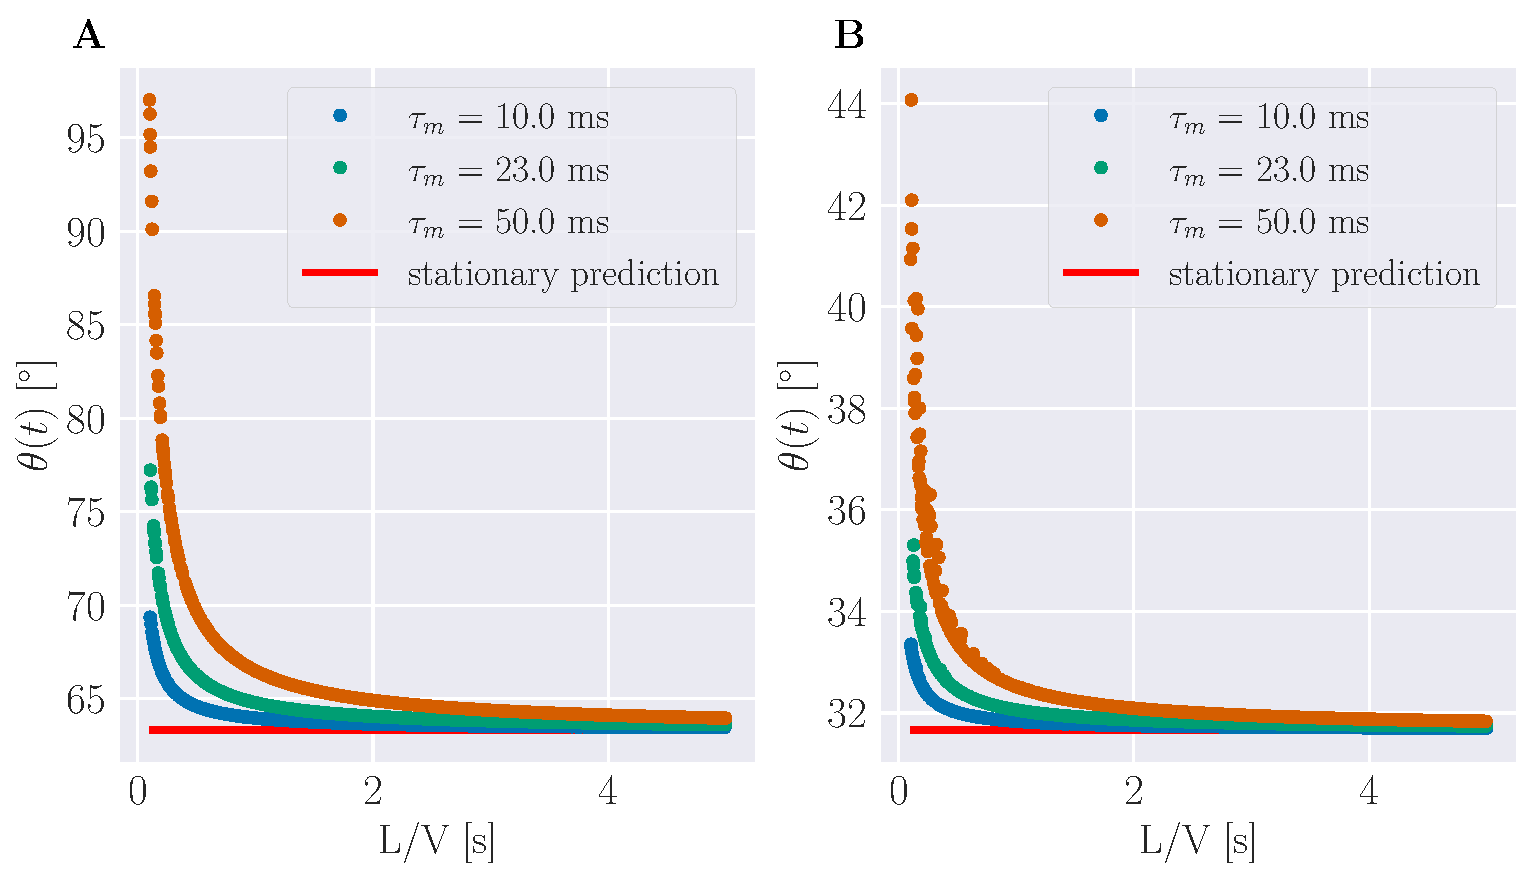
\includegraphics[width=\textwidth]{figure_station_inh_resp_angle.pdf}
    	\end{center}
    	\caption{\textbf{Response angles deviate from stationary solution for fast stimuli.} The response angle for the model with LIF dynamics and a stationary approximation of the inhibitory population activity is plotted against the L/V value of the stimulus using the same range of stimulus sizes L as in \cite{Bhattacharyya2017} (10 - 25 mm) but a larger range of L/V values. For the largest L/V values, the response angle closely matches the fully stationary solution and decreasing L/V leads to higher response angles than the stationary solution with a difference of about 25\% for the smallest L/V value and $\tau_{m}$ = 23 ms in \textbf{A}. Increasing the membrane time constant increases the deviations. The effect holds for different response angle levels (\textbf{A} and \textbf{B}).}
    	\label{fig:station_inh_resp_angle}
    \end{figure}
    
    \section{Full neuronal model}
    Coming back to the full neuronal model as described by equations \ref{eq:inhib}, \ref{eq:mcell} and \ref{eq:thrs} we have now additionally the time scale that the inhibitory population works on.
    This again leads to deviations from the stationary solution but for the inhibitory population the response angle decreases for faster stimuli because the inhibition lacks behind the excitation of the membrane potential.
    Effectively, this results in the same qualitative pattern that we saw in the previous section but with a decreased amount of deviation because the delays from the membrane time constant and the inhibitory population time constant compensate each other partially (compare Figure \ref{fig:full_model_resp_angle} and \ref{fig:station_inh_resp_angle}).
    But this only holds if we set the time constant of the inhibitory population $\tau_{\rho}$ to 1.
    We did this because studies of the auditory pathway suggest that the synapses of the feed-forward inhibition are electrical and therefore operate on a fast time scale.
    As this is not necessarily true for the visual pathway we also analyzed slower time scales for the inhibitory population and find that already for $\tau_{\rho}$ = 5 ms (and fixing $\tau_m$ = 23 ms) the deviation from the stationary response angle flips and we now have smaller response angles (Figure \ref{fig:full_model_effect_tau_inh}).\\
    These differences in the time delays between the different models are illustrated for a single trial with a slow and with a fast stimulus in Figure \ref{fig:voltage_traces}.
    For the slow stimulus (left column) all three model versions show similar voltage traces (bottom row) and therefore result in similar response angles.
    For the fast stimulus (right column) we see that in the full neuronal model the inhibitory input is slightly smaller than in the other two models where the inhibitory population activity is approximated by the stationary solution (blue line vs. green and orange in the second row from the top).
    This leads to a higher total effective input for the M-cell (blue line is higher in the third row from the top) and thus the membrane potential reaches the firing threshold earlier (bottom row) which means that the response angle is smaller than in the other two models (first row).
    On the other hand, for the stationary inhibition model the effective input for the M-cell is the same as in the fully stationary model (green and orange lines in the third row from the top) but due to the LIF dynamics with the membrane time constant the input is integrated with a delay so that the membrane voltage reaches the threshold later (bottom row) and thus the response angle is higher (top row).
    \begin{figure}[H]
    	\begin{center}
			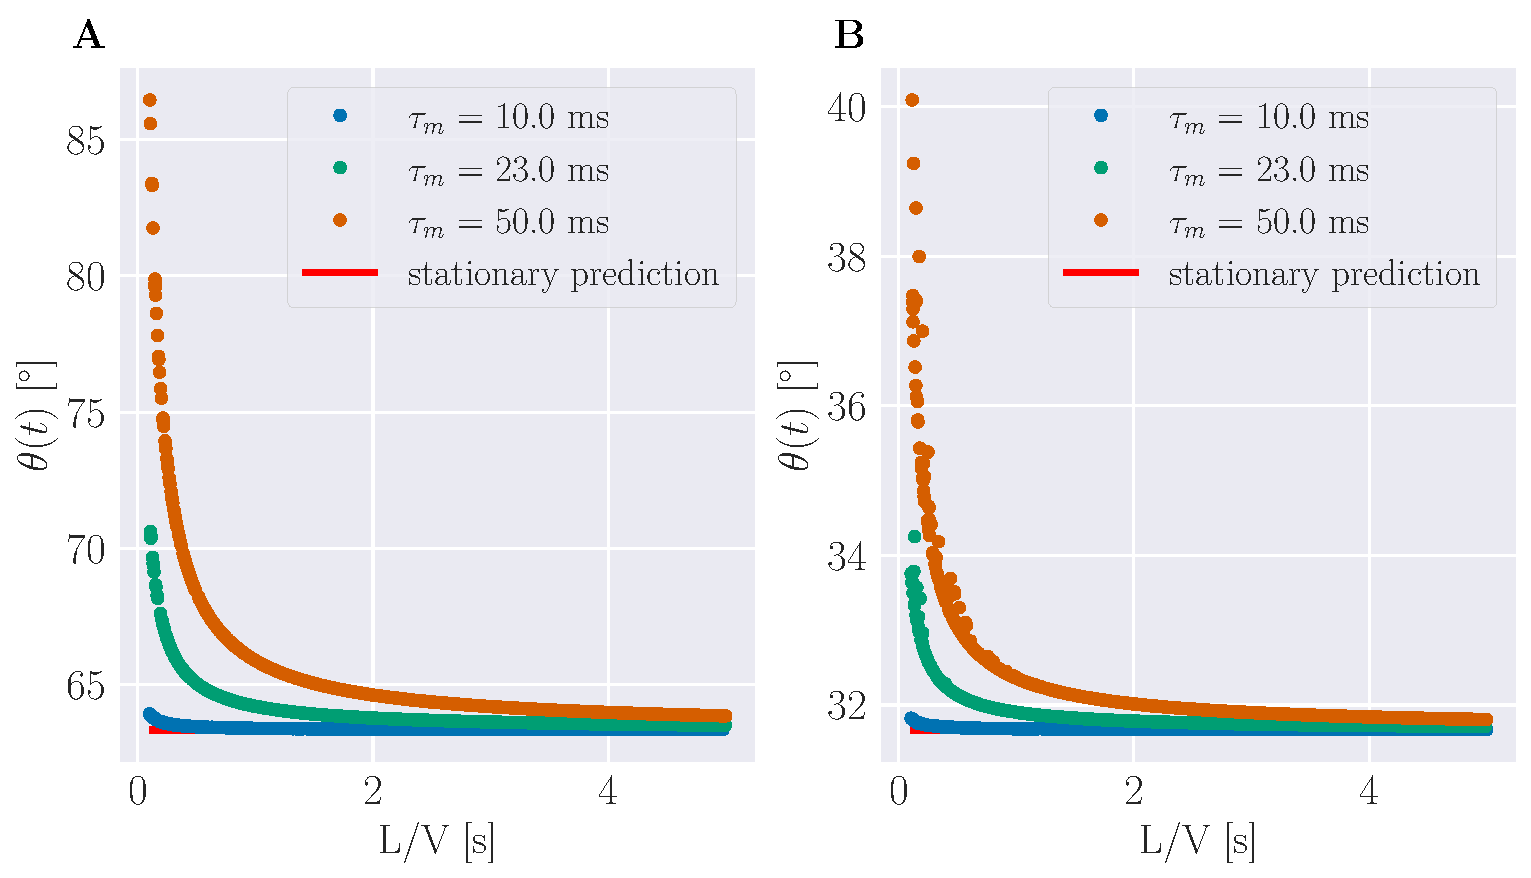
\includegraphics[width=\textwidth]{figure_full_model_resp_angle.pdf}
    	\end{center}
    	\caption{\textbf{Full model response angles deviate less from stationary solution.} The response angle for the full neuronal model is plotted against the L/V value of the stimulus using the same range of stimulus sizes L as in \cite{Bhattacharyya2017} (10 - 25 mm) but a larger range of L/V values. We see the same qualitative pattern as in Figure \ref{fig:station_inh_resp_angle} but here the deviations are less pronounced with a difference of only about 10\% for the smallest L/V value and $\tau_{m}$ = 23 ms in \textbf{A}. Increasing the membrane time constant increases the deviations. The effect holds for different response angle levels (\textbf{A} and \textbf{B}).}
    	\label{fig:full_model_resp_angle}
    \end{figure}
    
    \begin{figure}[H]
    	\begin{center}
			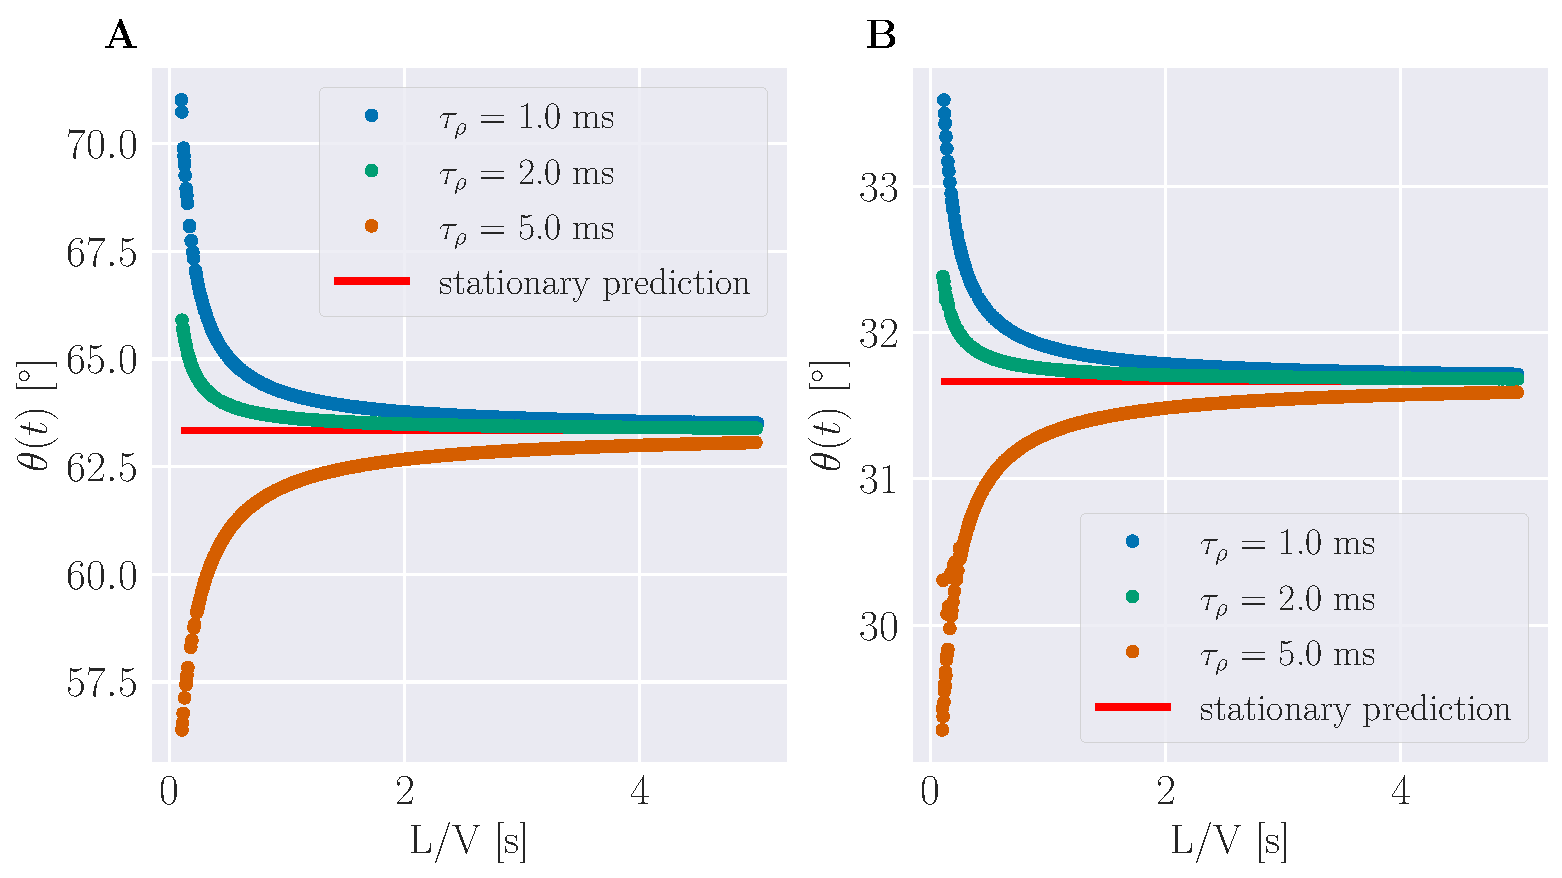
\includegraphics[width=\textwidth]{figure_full_model_resp_angle_tau_inh.pdf}
    	\end{center}
    	\caption{\textbf{Higher inhibitory time constants decrease the response angle.} Same setup as in Figure \ref{fig:full_model_resp_angle} but with $\tau_m$ = 23 ms and variable $\tau_{\rho}$. Increasing $\tau_{\rho}$ leads to lower response angles and at $\tau_{\rho}$ = 5 ms to response angles that are lower than the stationary solution. The effect holds for different response angle levels (\textbf{A} and \textbf{B}).}
    	\label{fig:full_model_effect_tau_inh}
    \end{figure}
    
     \begin{figure}[H]
    	\begin{center}
			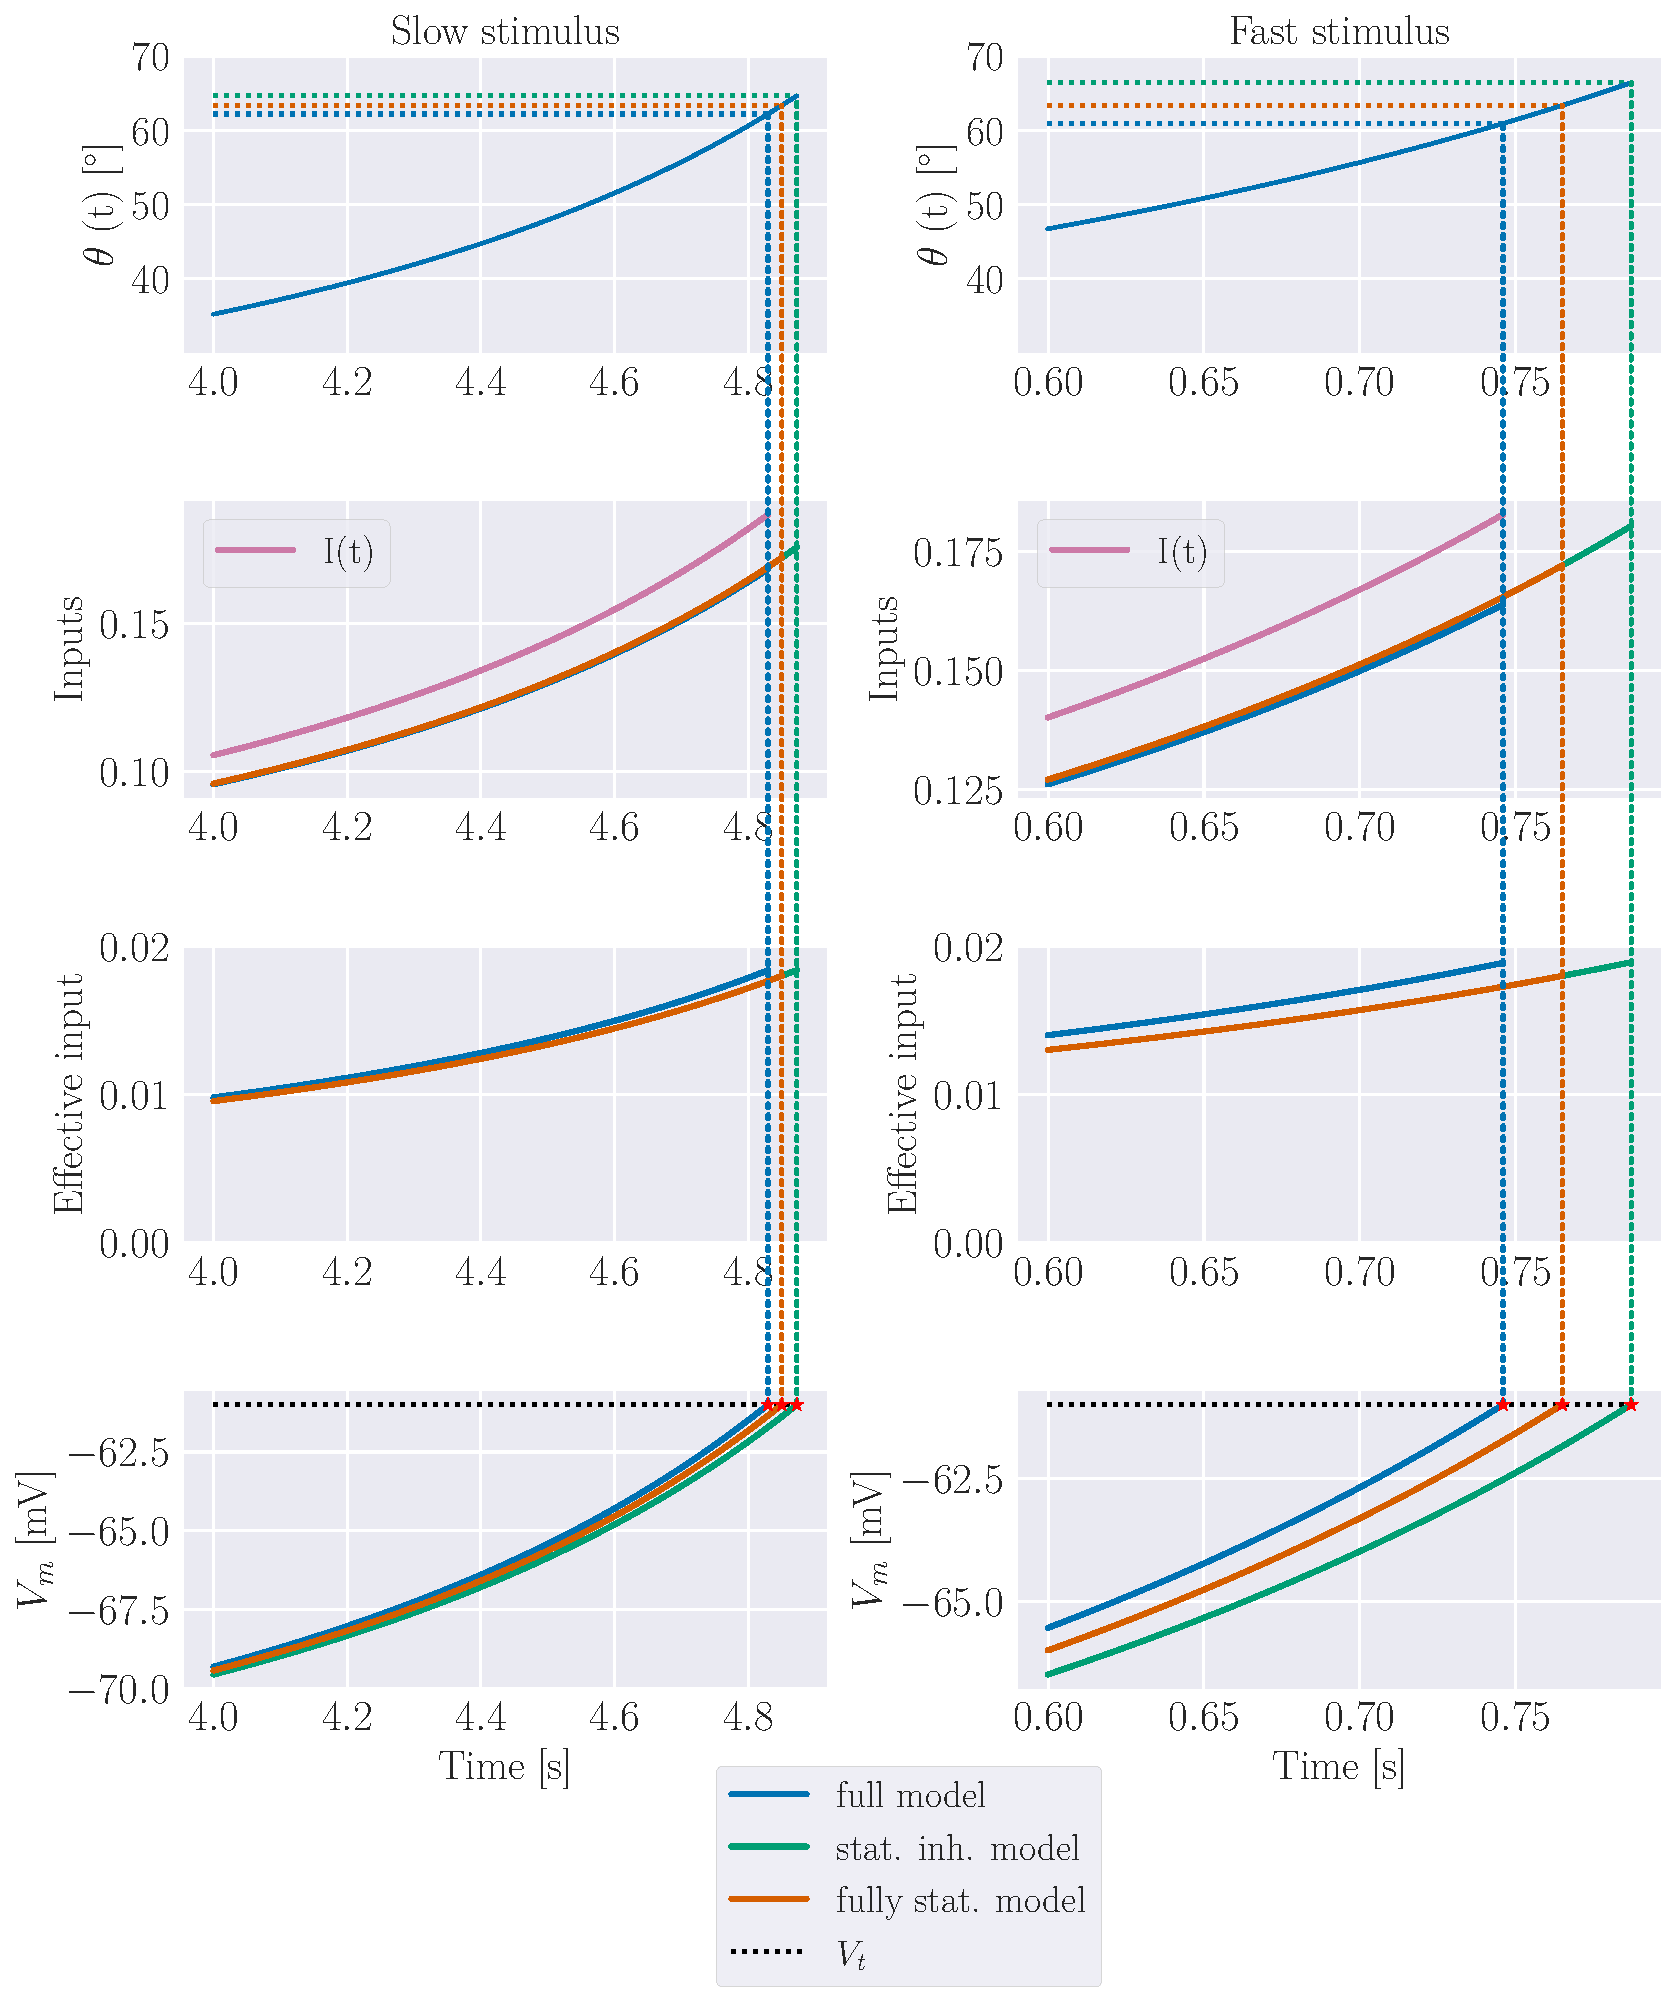
\includegraphics[width=\textwidth]{figure_voltage_traces.pdf}
    	\end{center}
    	\caption{\textbf{Single trial comparison of the different models for a slow and a fast stimulus.} Each of the two columns shows from top to bottom 1) the visual angle of the stimulus, 2) the excitatory and the inhibitory input for the M-cell, 3) the effective input for the M-cell and 4) the membrane voltage of the M-cell. While the models show very similar traces for the slow stimulus (left column), a fast stimulus leads to bigger differences in the resulting response angle.}
        %TODO: edit caption
    	\label{fig:voltage_traces}
    \end{figure}
    
    \section{Parameter fitting}
    In order to find out which parameter values account best for the observed response angles we fitted the full neuronal model to the data of \cite{Bhattacharyya2017} (see Figure \ref{fig:expm_theta_lv}).
    We used only this dataset because we have the response angles and the sampled L/V values for all trials instead of only the mean values of the response angle.
    Furthermore, since the study was done with zebrafish, we could use the fitted parameter values from \cite{Koyama2016} to constraint the model.\\
    For the fitting, we used the recently published library \textit{Delfi}, developed by \cite{Lueckmann2018}.
    The library implements several inference algorithms, from which we used the Sequential Neural Posterior Estimation (SNPE).
    Briefly, the algorithm uses a Mixture-Density Network (MDN) as a density estimator that approximates the true posterior distribution of the model parameters given the observed data.
    This is achieved by sequentially training the parameters of the MDN with data that is generated by the model using model parameters that are sampled from the current prior distribution.
    After such a training round the prior is updated to be the current estimated posterior distribution and this is repeated until the estimated posterior converges to the true posterior which can be evaluated by the importance-weighted log loss.
    For further details see \cite{Lueckmann2018} and the documentation of \textit{Delfi} (version 0.4.1) at \href{http://www.mackelab.org/delfi/}{http://www.mackelab.org/delfi/}.\\
    The parameters of the algorithm consist of the number of hidden layers of the neuronal network, the number of neurons for each layer, the number of rounds, the number of training trials for each round and the number training epochs.
    Here we used three hidden layers with 330 neurons each and trained for a single round of 40000 training trials with 100 epochs.\\
    In order to efficiently learn the mapping between the data and the posterior distribution we reduced the dimensionality of the raw data, which consisted of pairs of L/V values and response angles for 246 trials, by computing five quantile values (10\%, 30\%, 50\%, 70\% and 90\%) of the response angles in six bins for the L/V values resulting in 30 data points.
    How this reduction looks like for the data of \cite{Bhattacharyya2017} is shown in Figure \ref{fig:expm_data_to_quantiles}.\\
    \begin{figure}[H]
    	\begin{center}
			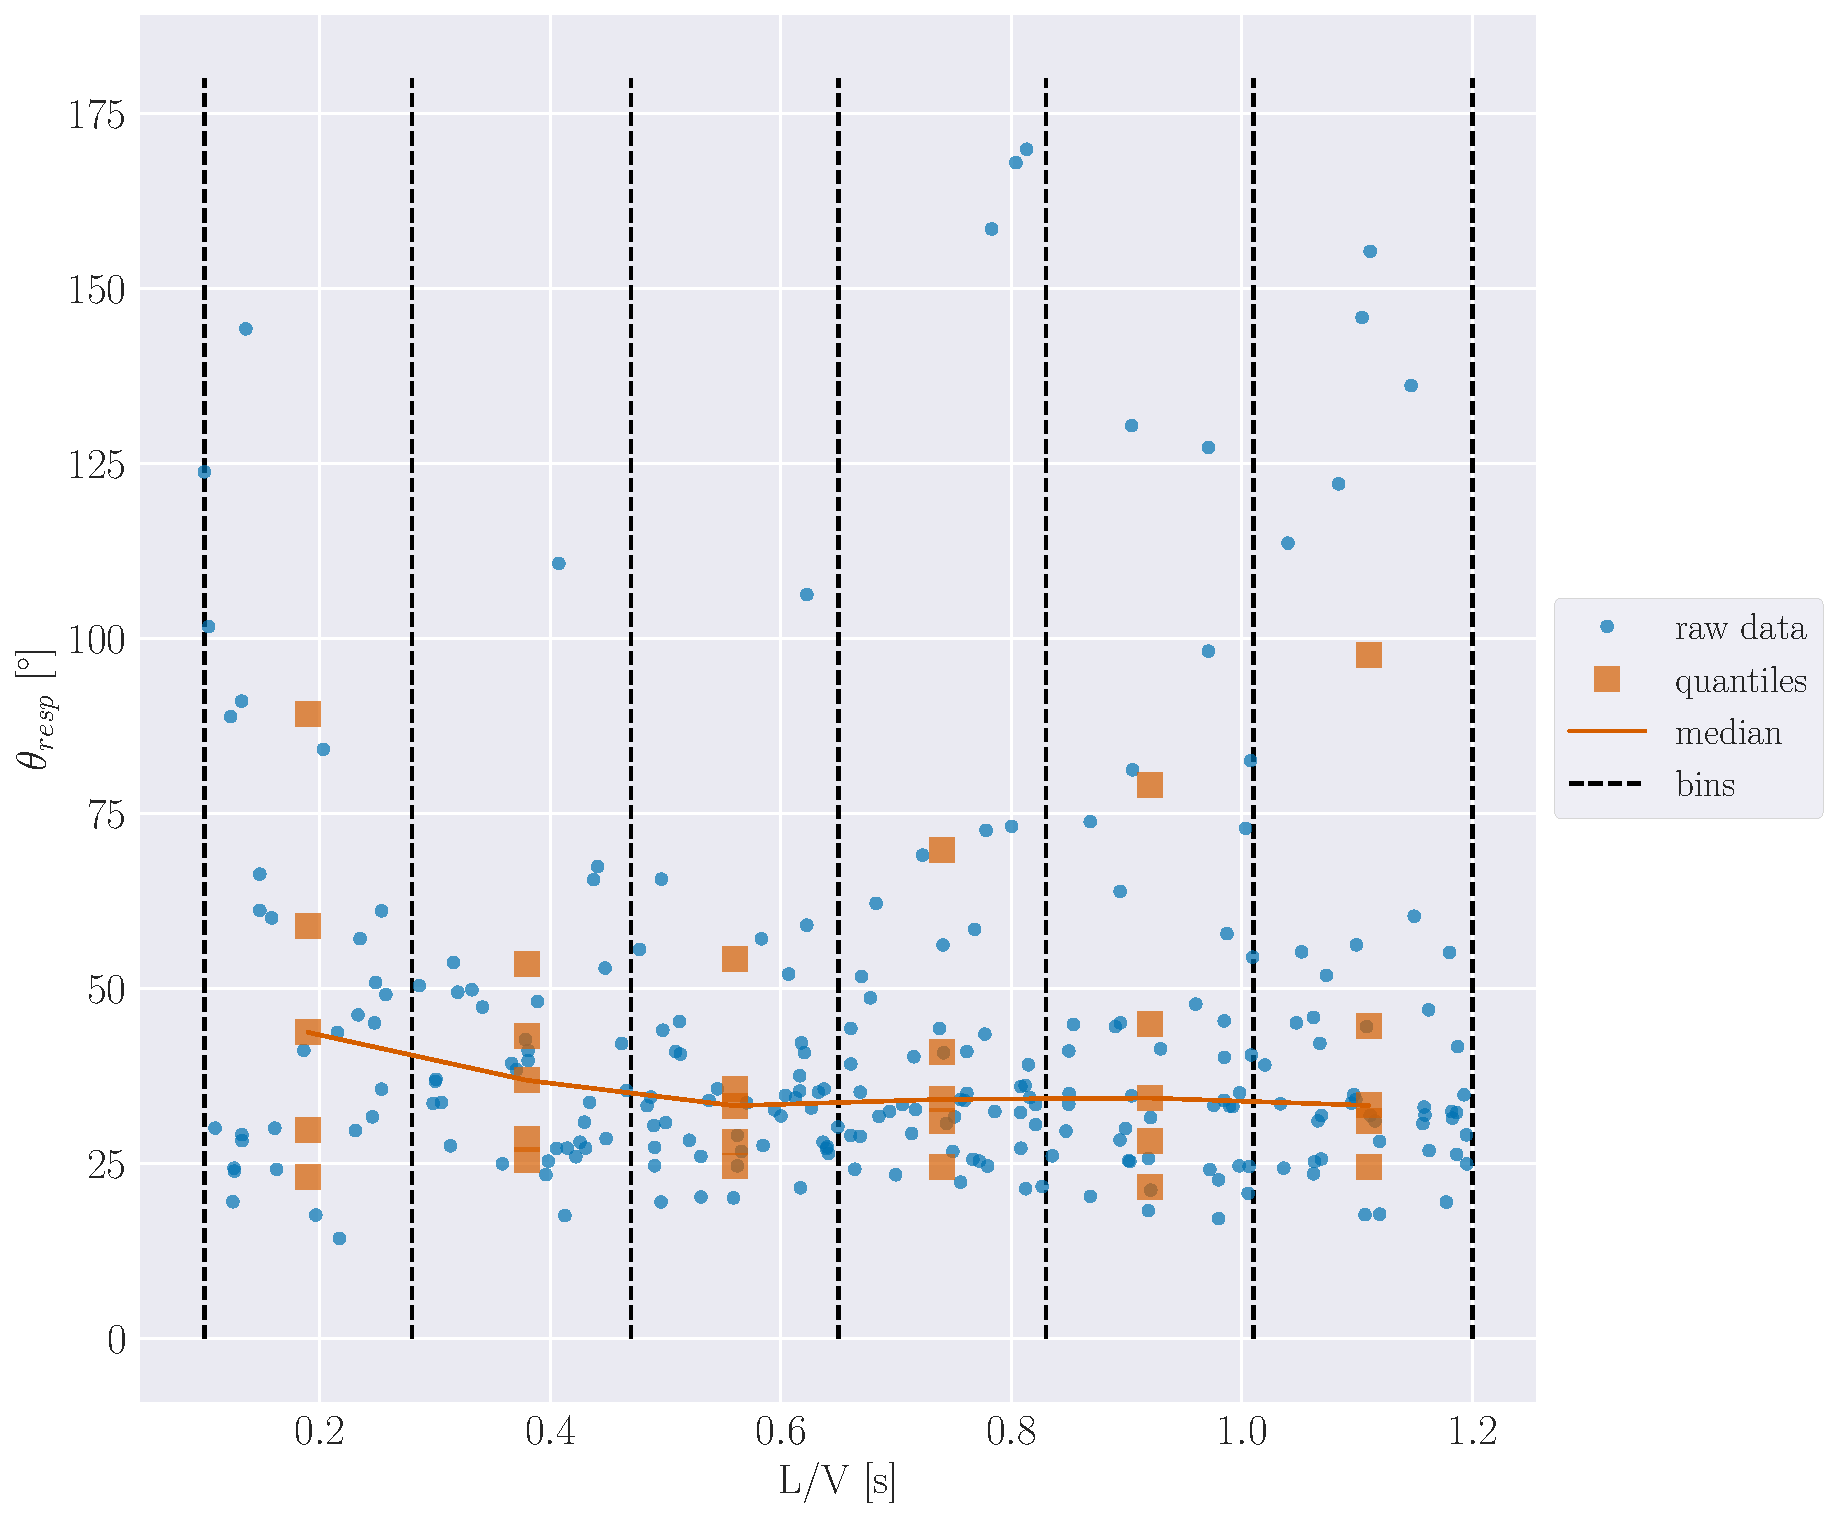
\includegraphics[width=\textwidth]{figure_data_to_quant.pdf}
    	\end{center}
    	\caption{\textbf{Data summary statistic for the fitting algorithm.} The range of L/V values (0.1 to 1.2) is divided in 6 bins and for each bin the 10\%, 30\%, 50\%, 70\% and 90\% quantiles are computed. The resulting quantile values are shown for the dataset of \cite{Bhattacharyya2017}.}
    	\label{fig:expm_data_to_quantiles}
    \end{figure}
    Out of the remaining 14 parameters after fixing the electrophysiological parameters of the M-cell at the values from \cite{Koyama2016}, we only fitted $\mu_{\rho_{0}}$, $\sigma_{\rho_{0}}$, $c_{\rho}$, and $\eta_{m}$.
    The remaining parameters are the trial time, the initial resting time, the simulation time step, the input scaling factor, the noise variances for the firing threshold and the inhibitory population, the time constant of the inhibitory population, the slope and offset of the linear transformation of the input and finally the cutoff angle.
    We fixed to 5 s and 2 s, resembling the corresponding times in the experiment.
    The simulation time step was set to 1 ms, which is enough to capture all relevant dynamics in the simulation.
    Setting the input scaling to $3 \cdot 10^{-10}$, the slope of the linear transformation to 3 and the offset to zero sets the baseline response angle to a medium value.
    We used a cutoff angle of 180\textdegree{} which is the maximal visual angle that is physically possible.
    We further assume a reasonable amount of noise with a standard deviation of 5 mV on the activation of the inhibitory population and set the time constant for the inhibitory population to 1 ms motivated by electrical synapses as described before.\\
    Since the algorithm uses Bayesian inference we need to define priors for the parameters that we want to fit.
    We chose uniform distributions for all parameters and the ranges were generally choses such that the model can result in very different patterns of response angle distributions but not too extreme.
    For the two parameters of the distribution of $\rho_0$ we chose the ranges 0 to 5 and 0.5 to 5 for the mean and variance respectively.
    This allows for for almost normally distributed values if both parameters are small or very skewed distributions if the variance is higher (see also Figure \ref{fig:effect_rho_null_stationary}).
    The range for the noise of the membrane potential is 0 to 5 which allows for practically no noise to very noise membrane potential traces.
    Finally, the prior for the inhibitory input scaling $c_{\rho}$ is a uniform distribution that goes from $5\cdot 10^{6}$ to $10\cdot 10^{6}$ where $5\cdot 10^{6}$ would correspond to very weak feed-forward inhibition and $10\cdot 10^6$ would mean that the inhibition fully compensates the excitation from the input.
    An overview of the fixed parameter values, the free parameters and their priors is given in Table \ref{tab:neuroparams}.\\
    As a first step we analyzed how well the fitting procedure would perform on model-generated data.
    We find that the algorithm performance differs between the model parameters but the overall performance is reasonable.
    On a positive note, the fitting results seem to be rather robust since the repetitions that we ran for each ground truth parameter set led to very similar fitted distributions (see the similarity between line "pairs" in each subplot in Figure \ref{fig:fit_validation}).
    The worst result among the single parameters is found for the variance of the membrane noise $\sigma_m$ where the fitted posterior means have all similar values regardless of the true parameter value and also high variances, indicating high probabilities for a wide range of values for $\sigma_m$ (Figure \ref{fig:fit_validation} D).
    For the mean of the distribution for $\rho_{0}$ the true values mostly lie within the standard deviation of the posterior distribution although here as well, the variances of the posteriors are rather high (Figure \ref{fig:fit_validation} A).
    The results for the variance of he distribution for $\rho_0$ are mixed.
    In two cases the posterior means almost perfectly match the true values but in three other cases the true values are underestimated by the posterior (Figure \ref{fig:fit_validation} B).
    Similarly, for the scaling factor of the input for the inhibitory population $c_{\rho}$, the posterior matches the true values rather good in two to three cases but deviates from the true value in the remaining cases (Figure \ref{fig:fit_validation} C).\\
    \begin{figure}[H]
    	\begin{center}
			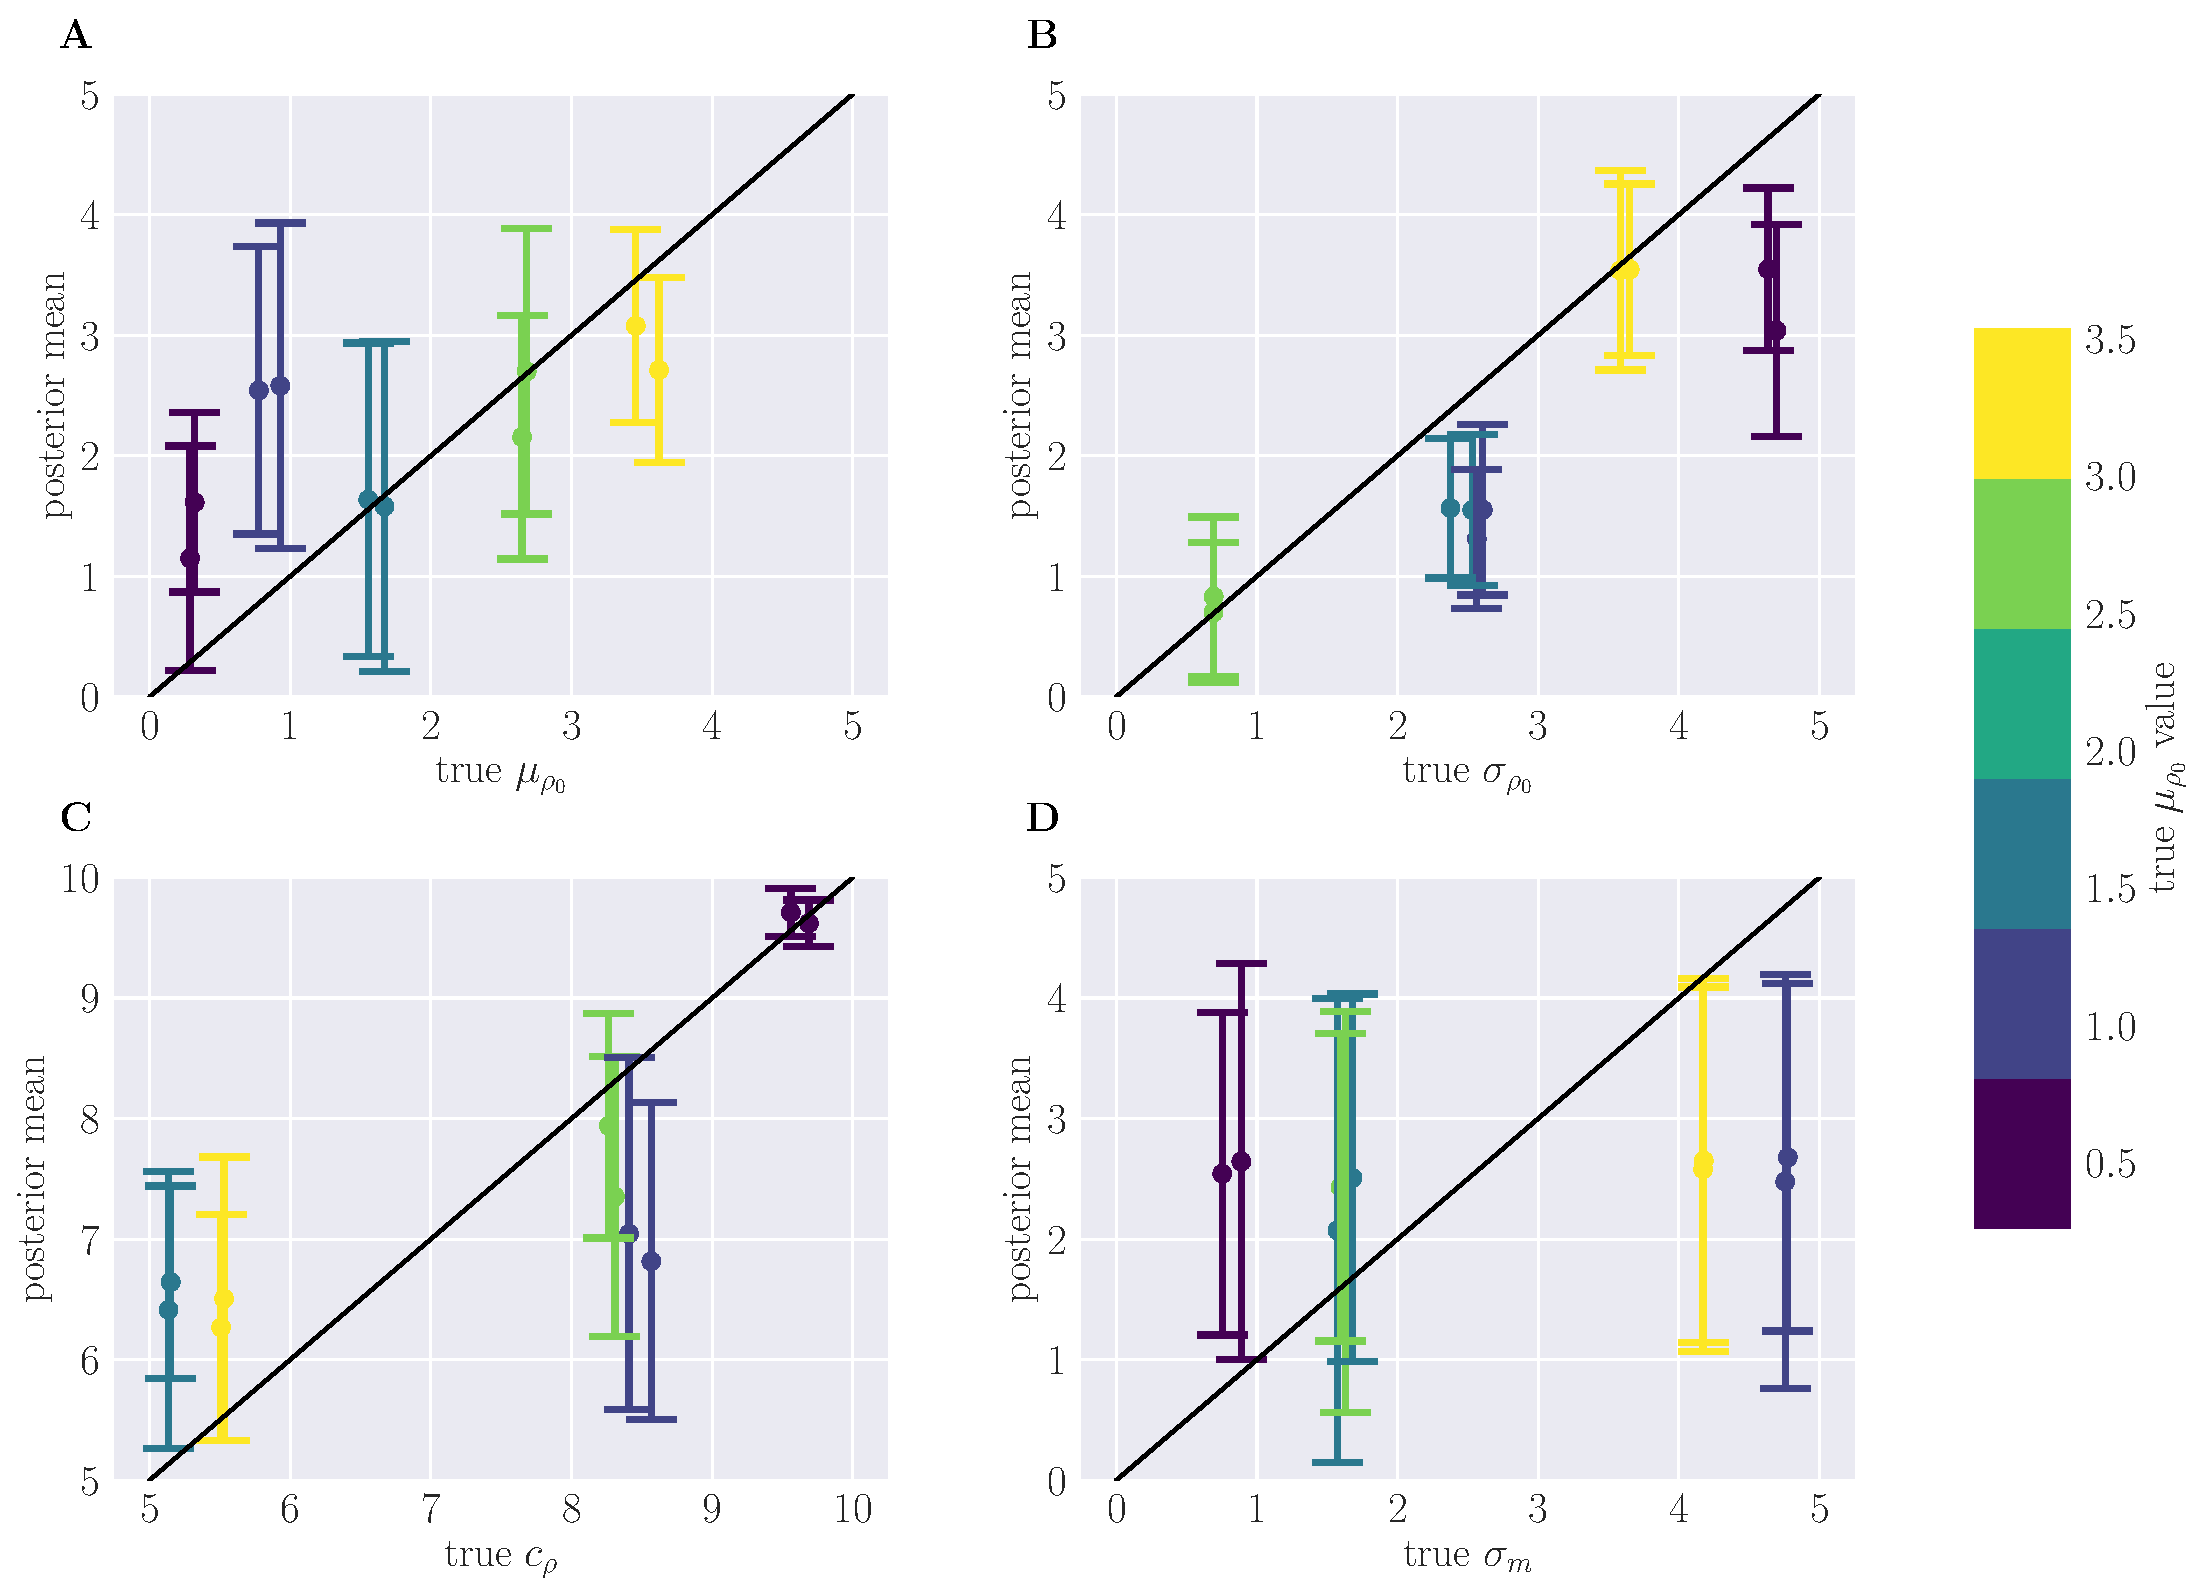
\includegraphics[width=\textwidth]{figure_fit_validation.pdf}
    	\end{center}
    	\caption{\textbf{Validation of fitting procedure.} For datasets that were generated by the model itself the posterior mean and standard deviation after fitting are shown. The posteriors have in general large variances. The parameters $\mu_{\rho_{0}}$, $\sigma_{\rho_{0}}$ and $c_{\rho}$ show the right tendency where larger true values correspond with larger posterior means. The fitted posteriors for the parameter $\sigma_{m}$ have all very similar mean values indicating that this parameter is not recoverable with the current parameter setting of the fitting procedure.}
    	\label{fig:fit_validation}
    \end{figure}
    In the next step we fitted the full neuronal model to the experimental data from \cite{Bhattacharyya2017}.
    The posterior distribution of the fit is shown in Figure \ref{fig:fit_expm_post}.
    As we have already seen in the parameter recovery from above, the posterior mean for the variance of the membrane noise lies in the middle of the prior range and has a high variance.
    This indicates that the exact value of $\sigma_m$ has no big influence on the resulting distribution of data.
    For the remaining parameters we find a rather narrow peak at $\mu_{\rho_0}$ = 3.6, $\sigma_{\rho_0}$ = 0.8 and $c_{\rho}$ = 8.2.
    How the data from the model with these fitted parameters compares to the experimental data is shown in Figure \ref{fig:fit_expm_comparison}.
    If we compare data for the same amount of trials as in the experiment we see a good match, especially for the lower range of response angles (Figure \ref{fig:fit_expm_comparison} A) whereas the model seems to have a higher density of response angles above 60\textdegree{} than in the experiment which is also reflected by the higher deviations for the 90\% quantiles in Figure \ref{fig:fit_expm_comparison} B.
    The higher accuracy for the lower range of response angles makes sense because there are more data points in this range so that the summary statistics are more informed in this range.
    \begin{figure}[H]
    \begin{center}
    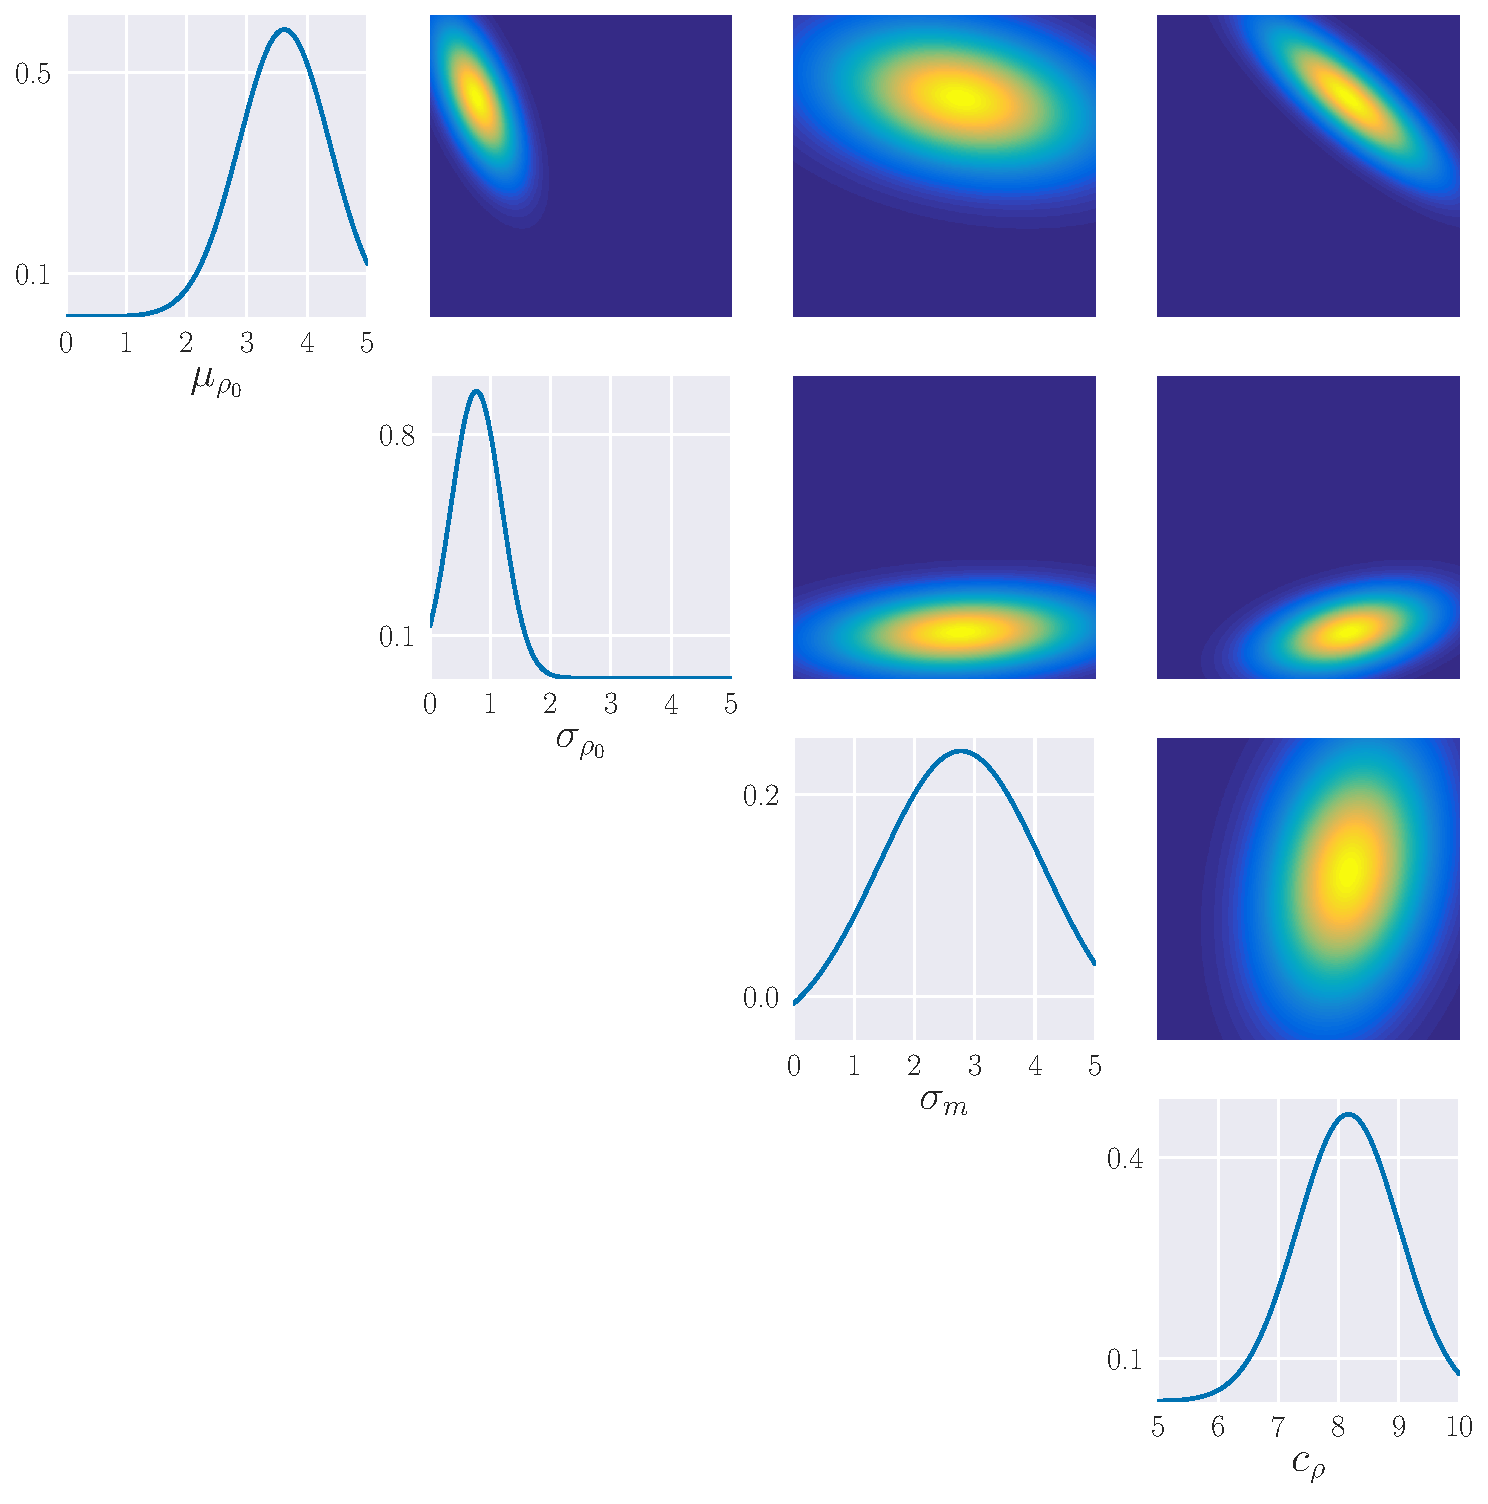
\includegraphics[width=\textwidth]{figure_expm_fit_posterior.pdf}
    \end{center}
    \caption{\textbf{The posterior distribution of the fitted parameters.} The distribution of $\sigma_{\rho_0}$ is the most narrow, indicating high certainty of the fitted mean value. In contrast, $\sigma_{m}$ has much wider distribution, speaking for little influence on the resulting fit. The covariances between $\mu_{\rho_0}$ on the one hand and $\sigma_{\rho_0}$ and $c_{\rho}$ on the other hand show negative correlations, i.e. for smaller values of $\mu_{\rho_0}$ it is more likely for $\sigma_{\rho_0}$ and $c_{\rho}$ to have higher values.}
    \label{fig:fit_expm_post}
    \end{figure}
    
    \begin{figure}[H]
    \begin{center}
    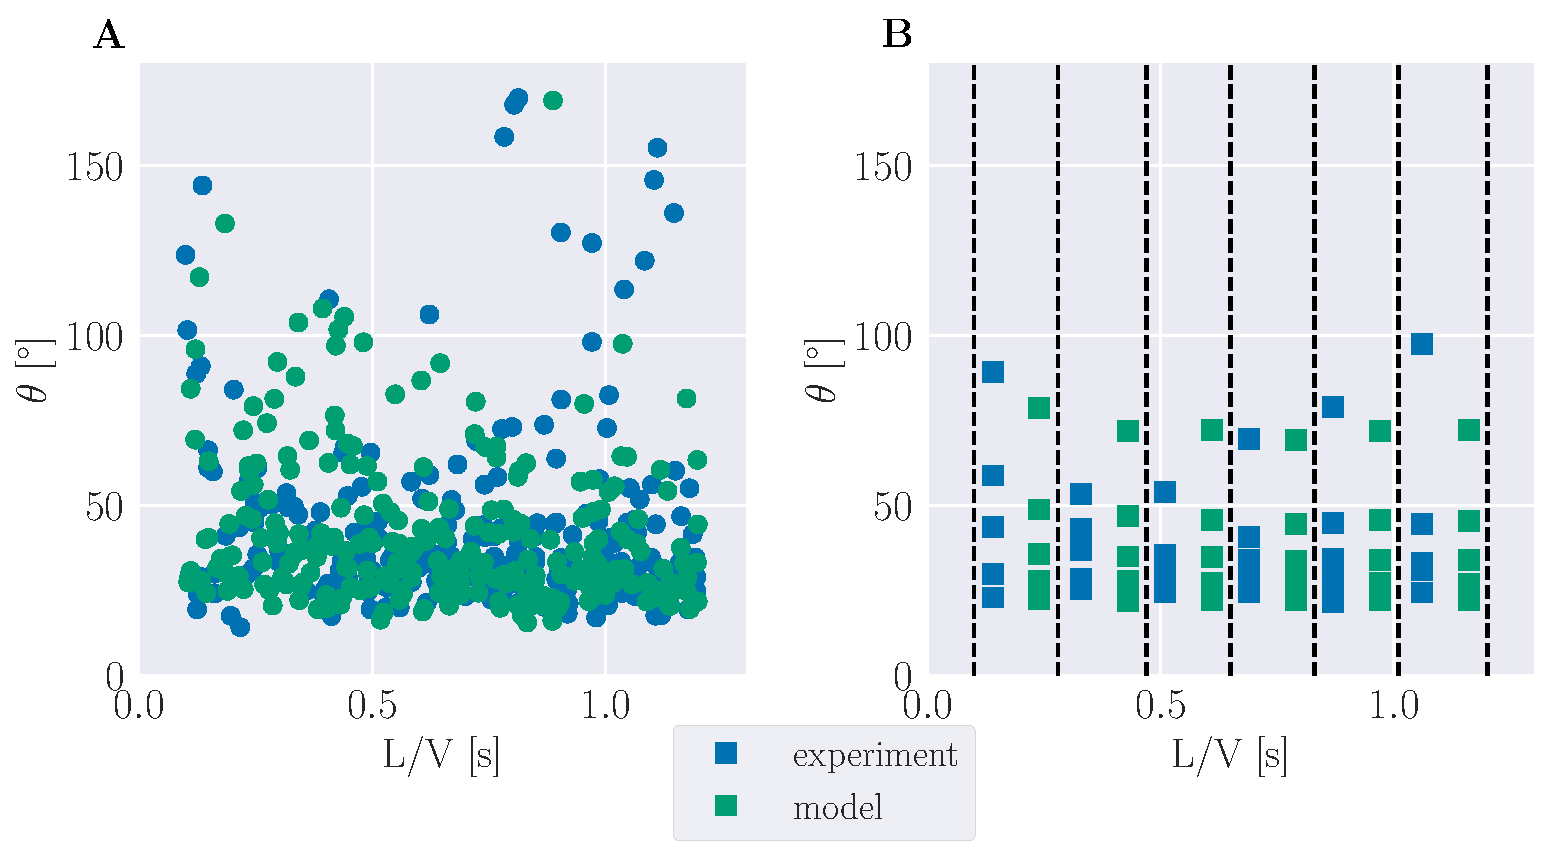
\includegraphics[width=\textwidth]{figure_expm_fit_comparison.pdf}
    \end{center}
    \caption{\textbf{Comparison of experimental data with data generated from the fitted model.} \textbf{A} Response angle data from \cite{Bhattacharyya2017} in blue and data from the same amount of trials generated by the fitted model in green are shown. While the two closely match for the lower range of response angles (20\textdegree{} - 60\textdegree{}), the model seems to generate more response angles in the range of 60\textdegree{} to 100\textdegree{} although this could look very different for different set of trials. \textbf{B} The quantiles of the experimental data and the average quantiles of 100 repetitions from the model. The first three to four model quantiles closely match the experimental data with some differences between the different bins. The last quantile shows larger deviations from the experiment.}
    \label{fig:fit_expm_comparison}
    \end{figure}
    \section{Discussion}
    In this chapter, we briefly reviewed experiments on startle responses evoked by looming visual stimuli, showed effects of the model parameters when we simulate the looming stimulus experiment for the different levels of approximations of the model dynamics and finally fitted a subset of model parameters to experimental data.\\
    The looming stimulus experiments that we considered here have many differences in their experimental conditions such as e.g. the arena setup including the position of the display and also the range of stimulus parameters L and V (see Table \ref{tab:looming_exp}).
    This is also reflected in the differences that we see for the measured response angles plotted against L/V although one should note that for the studies by \cite{Dunn2016} and \cite{Preuss2006} the shown data points are only the mean values so we don't know the underlying distribution (see Figure \ref{fig:expm_theta_lv}).
    It would therefore be desirable to have a more systematic study of startle responses evoked by a looming stimulus.
    Especially interesting to see would be experiments with higher stimulus velocities (or smaller L/V values) than were used in \cite{Bhattacharyya2017} because only for these stimuli the dynamics of the Leaky Integrate-and-Fire model and of the inhibitory population activity become relevant and we see deviations from stationary model versions (see e.g. Figure \ref{fig:full_model_effect_tau_inh}).
    If we consider for example the data from \cite{Temizer2015} it could be argued that the response angles tend to go down for smaller L/V values if we compare them to the response angles from \cite{Bhattacharyya2017} and in our model this could speak for a bigger time constant of the inhibitory population where we also see decreasing response angles for smaller L/V values (Figure \ref{fig:full_model_effect_tau_inh}).
    On the other hand, the differences might as well be explained by different experimental conditions and thus a study that examines a wider range of L/V values would be necessary to test this hypothesis.
    Furthermore, these considerations only hold under the assumption that our model is indeed approximating the true underlying mechanism that is responsible for the startle response initiation which we cannot say with much confidence as of now.\\
    This leads us to possible limitations of the model.
    The first point to mention here is the form of the visual input which we modeled as a linear transformation of the visual angle.
    Even if we accept that the visual angle is computed somehow it might well be that it undergoes a different, possibly nonlinear transformation before it reaches the the hindbrain such as e.g. a sigmoidal function.
    Regarding the computation of the visual angle there have been studies that show looming-sensitive neurons in locusts \citep{Hatsopoulos1995}, barn owls \citep{Mysore2010} and in bluegill sunfish as well as goldfish \citep{Gallagher2006} where for the barn owl and the two fish species they were found in the optic tectum.
    Ideally, we would have evidence for looming-sensitive neurons in the optic tectum of zebrafish and, even more important, recordings that show the activity during a looming stimulus in the presynaptic neurons of the M-cell.
    Such experiments have not been conducted so far to the best of our knowledge.
    Another thing to keep in mind in this context is, that the optic tectum of the larval zebrafish is still developing and this development has recently been shown to be affected by visual experience \citep{Avitan2017}.
    So it would also be interesting to investigate possible differences between larval and adult zebrafish.
    In all studies that we considered here, larval zebrafish were used.\\
    In the last part of this chapter we fitted the full neuronal model to the experimental data from \cite{Bhattacharyya2017} using an Approximate Bayesian Computation approach where a Mixture-Density-Network was employed to learn the mapping between response angle data and parameters of the posterior distribution of the model parameters.
    The results of the validation (Figure \ref{fig:fit_validation}) of the fitting procedure are not convincing yet as we saw large deviations from the ground truth parameters.
    Nevertheless, when we fitted the model to the experimental data, the model-generated data strongly resembles the experimental data (Figure \ref{fig:fit_expm_comparison}).
    Furthermore, there are several ways to improve the fitting procedure.
    One way would be to optimize the parameters of the fitting procedure such as the number of rounds, the number of generated training data per round, different architectures of the MDN and the number of components of the MDN.
    The parameters that we used here were the result of a small preliminary exploration that was limited by time constraints so that a more systematic exploration will likely lead to improvements.\\
    There are several possible extensions based on the presented work so far.
    In a first category of extensions we can use more and different kinds of data to further constraint and test the model.
    As an example, the fish are not always reacting with a startle response to a looming stimulus and the response probability has been found to differ for different L/V values by \cite{Bhattacharyya2017} and \cite{Temizer2015}.
    Such trials without a response also happen in our model and thus the response probability could be included in the fitting procedure.
    Another additional data set would be experiments where the visual angle of the stimulus follows other trajectories, e.g. a linearly increasing visual angle which has been already studied by \cite{Dunn2016}.
    Here it would also be interesting to compare the fitted parameters with those that were fitted to experiments with hyperbolically increasing visual angles as we did in this work and to see if both kinds of experiments result in the same fitted model parameters.
    To further constraint the model, one could use electrophysiological data in order to e.g. get an estimate of the amount of noise in the membrane potential.
    It should also be considered that the values for the electrophysiological model parameteres that were fitted by \cite{Koyama2016} might change for different experimental conditions and it would help to have several independent estimates of those parameters.\\
    Apart from using additional data, further work could also extend the neuronal model.
    One possible way would be to use a multi-compartment model for the Mauthner cell where the lateral dendrite, the ventral dendrite, the soma and the axon cap are obvious candidates for compartments in such a model.
    This would also make sense as a recent study found differential processing properties for the two main dendritic branches of the M-cell \citep{Medan2017}.
    The axon cap is another segment of interest as it is targeted by the excitatory input from the spiral fiber neurons \citep{Lacoste2015} and it is also the site of electrical inhibition \citep{Weiss2008}.\\
    A second way to extend the model would be to consider both M-cells that exist in the fish hindbrain.
    This would open up another set of interesting questions, e.g. how the fish would react to two stimuli coming from both sides leading to a competition between the two M-cells.
    How this competition might work has already been hypothesized by \cite{Koyama2016} but they only considered stimuli from one side and they did not use their model to explain response angle data.\\
    %TODO: check if this previous sentence is true
    An advantage of the fitting procedure that we used is that we can simply plug in these extended models to fit the same data.
    Furthermore, the Bayesian framework in principle also allows for model comparisons (see e.g. \href{https://github.com/janfb/mcabc}{https://github.com/janfb/mcabc} for an implementation) so that we are able to answer whether the supposedly more realistic models are also more likely to produce the observed data.
	\begin{table} [!th]
		\begin{center}
			\begin{tabular}{l|c|p{7cm}}
				%\hline
                \multicolumn{3}{c}{\rule{0pt}{4ex}\textbf{Fixed Parameters}}\\
                \textbf{Parameter} & \textbf{Value (unit)} & \textbf{Comment} \\
				\hline
				$E_L$ & -79 mV & Resting potential\\
				$R_M$ & 10 MOhm & Membrane resistance\\
				$\tau_{m}$ & 23 ms & Membrane time constant\\
				$V_t$ & -61 mV & Mean spiking threshold\\
				$dt$ & 0.001 s & Integration time step\\
				$T$ & 5 s & Total time\\
                $T_{init}$ & 2 s & Initial time of constant stimulus size\\
                $c_{scale}$ & $3 \cdot 10^{-10}$ & Scaling from visual angle to input current\\
				$\sigma_{t}$ & 0 mV & Standard deviation of spiking threshold noise\\
				$\sigma_{\rho}$ & 5 mV & Standard deviation of noise from inhibitory population\\
                $\tau_{\rho}$ & 1 ms & Time constant of the inhibitory population\\
				$m$ & 3  & Slope of linear transformation\\
				$b$ & 0 \textdegree & Offset of linear transformation\\
                $\theta_{cutoff}$ & 180 \textdegree & Cutoff visual angle\\
            \end{tabular}
            
            \begin{tabular}{l|c|c|p{6.1cm}}
                \multicolumn{4}{c}{\rule{0pt}{4ex}\textbf{Fitted Parameters}}\\
                \textbf{Parameter} & \textbf{Prior} & \textbf{Posterior} & \textbf{Comment} \\
				\hline
				$\mu_{\rho_0}$ & 0 - 5 & 3.6 & Mean of $\rho_0$ distribution\\
                $\sigma_{\rho_0}$ & 0.5 - 5 & 0.8 & Variance of $\rho_0$ distribution\\
                $\sigma_{m}$ & 0 - 5 & 2.7 & Standard deviation of noise from membrane potential\\
                $c_{\rho}$ & 5 - 10 & 8.2 & Input scaling for inhibitory population activity\\
				%\hline
			\end{tabular}
		\end{center}
		\caption{Fixed and fitted parameters of the full neuron model.}
		\label{tab:neuroparams}
	\end{table}


\chapter{Coupling of Neuronal Model and Collective Dynamics}
    \section{Collective Behavior Experiments}
    The mechanisms that underly the dynamics of collective behavior as we observe it in many species like birds or fish have been of great interest.
    Theoretical work that has been developed to explain the observed behavior often relies on agent-based models with local interaction rules (\cite{Couzin2002}, \cite{Vicsek1995}).
    Recently, \cite{Strandburg-Peshkin2013} investigated the nature of these local interactions by performing an experiment with a fish school of 70 fish where a part of the group has been trained to move to a stimulus so that they could function as leaders of the group from which the information about the stimulus would spread during the experiment.
    By comparing different models to explain the spread of information in the group, which was approximated by the measured response times of the individuals, they found that a model that was based on visual input was supported the most by the observed data.\\
    In another experiment, \cite{Rosenthal2015} found that visual input also plays a crucial role in the spread of startle responses in a fish school.
    For this, they analyzed spontaneously occurring startle events in a fish school of roughly 150 golden shiners and looked at the factors that were most predictive of a fish to startle after the initial startle event.
    The two most predictive features that they found were the logarithmic distance to visible neighbors and the rank of subtended angular area of the initially startling fish on the retina of the focal fish \citep{Rosenthal2015}.
    Note, that due to the elongated body shape of the fish and the location of the eyes on the side, the subtended angular area is different from the distance alone because for example, a neighboring fish that is in front of the focal fish might be closer but it will cover a smaller part of the visual field than compared to a neighboring fish on the side.
    In the case of several neighbors, occlusions will also influence the ranking of the subtended angular areas.
    Based on these features \cite{Rosenthal2015} constructed an interaction network of the fish school and found that the local weighted clustering coefficient at the moment of an initial startle is informative of the size of the following cascade of startles.\\
    The first aspect of the startle behavior of the fish school that we were interested in was the frequency of spontaneously occurring startles.
    In the experiment of \cite{Rosenthal2015} the total number of 138 such startle events was acquired from recordings of 5 different groups over 53 minutes each so that the startling frequency of the group is around $8\cdot 10^{-3}$ startles per second and around $5\cdot 10^{-5}$ for an individual fish.
    A similar experiment that was done with 40 instead of 150 golden shiners found that the spontaneous startling frequency is around $5\cdot 10^{-4}$ to $1\cdot 10^{-3}$ for a single fish (Matt Grobis, Couzin Lab, private communication) and thus an order of magnitude higher than in the experiment of \cite{Rosenthal2015}.
    A possible explanation for the lower startling frequency in the bigger fish school might be a decreased responsiveness that is caused by the presence of other fish as it has been found in Guppies \citep{Fischer2015}.
    \section{Collective Behavior Model}\label{swarm_methods}
    In this section we will describe the model for the collective behavior, the integration of the neuronal model for the startle response initiation, the behavioral measurements and give an overview of the implementation.
	The model describes the individual motion of an agent by a stochastic differential equation that includes Brownian motion as described in \cite{Romanczuk2012a} and a continuous version of social interaction as described in \cite{Couzin2002}.
	We assume a set of $N$ interacting agents ($i= 1,\dots, N$).
	The dynamics of each agent in 2D is described by the following equations of motion:

	\begin{equation}
		\frac{d \vec{r}_i}{dt}=\vec{v}_i(t)
		\label{eq:r_diff}
	\end{equation}
	
	\begin{equation}
		\vec{v}_i(t) = {s_i\cos(\varphi_i(t)) \choose s_i\sin(\varphi_i(t)) }
		\label{eq:v_def}
	\end{equation}
	
	\begin{equation}
		\frac{d s_i}{dt} = \alpha\left( \mu_{s} - s_i\right) + F_{i, s} + \eta_{i, s}
		\label{eq:s_diff}
	\end{equation}
	
	\begin{equation}
		\frac{d \varphi_i}{dt} = \frac{1}{s_i + c_{s}}\left( F_{i,\varphi} + \eta_{i,\varphi} \right)
		\label{eq:phi_diff}
	\end{equation}
	
	Here $\vec{r}_i$ is the Cartesian position vector and $\vec{v}_i$ is the velocity vector, both of the focal agent.
	In the absence of social forces the speed $s_i$ of agent $i$ is relaxing towards the mean value $\mu_{s}$, which is the same for all agents, while we add the Gaussian white noise term $\eta_{i, s}$ and the relaxation time is determined by $\alpha$.
	The influence of the total effective social force is calculated by the projection onto the normalized velocity vector:
	
	\begin{equation}
		F_{i, s}=\vec{F}_i \cdot \vec{u}_{v, i} = \vec{F}_i { \cos\varphi_i \choose \sin\varphi_i }
		\label{eq:s_force}
	\end{equation}
	
	The change of direction $\varphi$ is mostly determined by $\vec{F}_{i,\varphi}$, the projection of the total effective social force onto the orthogonal of the normalized velocity vector and added Gaussian white noise represented by $\eta_{i,\varphi}$.
	
	\begin{equation}
		F_{i,\varphi}=\vec{F}_i \cdot \vec{u}_{\varphi,i} = \vec{F}_i {-\sin\varphi_i \choose \cos\varphi_i }
		\label{eq:phi_force}
	\end{equation}
	
	Additionally, we introduce the term $1/(s_i + c_s)$ to decrease the amount of direction change for high speeds where $c_s$ is meant to prevent numerical instabilities for very small $s_i$ values.
	The stochastic differential equations for the direction of motion of individual agents can be solved by a simple Euler-Maruyama method:
	
	\begin{equation}
		\varphi_i(t+1) = \varphi_i(t) + \frac{1}{s_i}\left( F_{i,\varphi}(t)\Delta t + \sqrt{2 \sigma_{\varphi}\Delta t} \text{ GRN(t)}\right)
		\label{eq:phi_update}
	\end{equation}
	
	\begin{equation}
		s_i(t+1) = s_i(t) + (\alpha (\mu_s - s_i(t)) + F_{i, s}(t))\Delta t + \sqrt{2 \sigma_{s} \Delta t} \text{ GRN(t)}
		\label{eq:s_update}
	\end{equation}
	
	\begin{equation}
		\vec{r}(t+1) = \vec{r}(t) + {s_i\cos(\varphi_i(t)) \choose s_i\sin(\varphi_i(t)) }
		\label{eq:r_update}
	\end{equation}
	Here "GRN(t)" is a Gaussian Random Number drawn from the standard normal distribution and $\sigma_\varphi$ and $\sigma_s$ are the standard deviations of direction and speed noise respectively.
	The total effective social force is a sum of three components:
	\begin{equation}
		\vec{F}_i=\vec{F}_{i,rep}+\vec{F}_{i,alg}+\vec{F}_{i,att}
		\label{eq:forces}
	\end{equation}
	Attraction:
	\begin{equation}
		\vec{F}_{i,att}= \frac{1}{n_{i,att}}\sum_{j \in Neigh} \mu_{att}S_{att}({r}_{ji}) \hat{r}_{ji}
		\label{eq:att}
	\end{equation}
	Repulsion:
	\begin{equation}
		\vec{F}_{i,rep}=\frac{1}{n_{i,rep}}\sum_{j \in Neigh} -\mu_{rep}S_{rep}({r}_{ji}) \hat{r}_{ji}
		\label{eq:rep}
	\end{equation}
	Alignment:
	\begin{equation}
		\vec{F}_{i,alg}=\frac{1}{n_{i,alg}}\sum_{j \in Neigh} \mu_{alg}S_{alg}({r}_{ji}) (\vec{v}_j-\vec{v}_i)
		\label{eq:alg}
	\end{equation}
	with $\vec{r}_{ji} = \vec{r}_j - \vec{r}_i$, $r_{ji} = |\vec{r}_{ji}|$ and $\hat r = \vec{r}/|r|$.
	Each component is computed by the normalized sum over the forces of the single interaction pairs with all agents of the neighborhood of the focal agent.
	For the metric interaction the neighborhood consists of all other agents and for the topological interaction the neighborhood consists of the Voronoi neighbors (for explanation, see Introduction).
	Note that the interaction range of the metric interaction is implemented by the weighting functions $S_X(r)$ that are sigmoid functions of distance, which go from 1 to 0, with the transition point at $r_{X,0}$ and steepness $a_{X}$:
	\begin{equation}
	S_X(r)=\frac{1}{2}\left(\tanh(-a_{X}(r-r_{X,0})+1\right)
	\label{eq:sigm}
	\end{equation}
	The strength of the different interactions is set by a constant $\mu_X$.
	For the normalization we use the number of effective neighbors $n_{i,X}$ which we define as the number of neighbors for topological interaction and for metric interaction we take the sum of the values of $S_X(r)$ so that $n_{i,X}$ will be approximately the number of agents within the interaction range:
	\begin{equation}
	n_{i,X} = \left\{\begin{array}{lc}
	|\{j, j \in Neigh\}|, & \text{for topological interaction}\\
	\sum_{j \in Neigh} S_X(r_{ji}), & \text{for metric interaction}
	\end{array}\right.
	\label{eq:neigh}
	\end{equation}\\
	Note, that due to numerical precision the numerical value returned by $S_X(r)$ is equal to zero for analytical values that are smaller than double precision which is in the order of $10^{-16}$.
	To avoid division by zero, we apply the normalization only for agents whose numerical value of $n_{i,X}$ is not zero.
	This also means that the ranges for the social forces are effectively longer since the normalization will rescale all non-zero values returned by $S_X(r)$ to the order of one.
	For the simulation of the fish school we define the basic time unit as seconds and the basic distance unit as one body length (BL) of a fish.
	We use a square arena of size $L$ with periodic boundaries so that the effective topology of the arena is a torus.
	\subsection{Coupling with neuronal model}
	For each agent we use the full neuronal model as described by equations \ref{eq:inhib} to \ref{eq:thrs} to initiate startle responses during the simulation.
    The resting activity of the inhibitory population $\rho_{0}$ of each agent was set to the mode of the fitted log-normal distribution from the previous chapter which was approximately $20.6$ in our case.
    For all other neuronal parameters we took the values that were either fixed or fitted in the previous chapter (see Table \ref{tab:neuroparams}).\\
    The last part that we need to define for the coupling is the visual input.
    In the previous chapter we had an abstract situation with only one stimulus but in the collective behavior simulations the agents are possibly surrounded by many neighbors.
    We considered three different methods to determine the effective visual input: max, k-nearest neighbors (KNN) and k-nearest mean deviate (KMD).
    For all methods we first computed the visual angle of each neighbor of the focal agent by assuming that the shape of an agent is a sphere with a diameter of one body length.
    Then, for the max method we simply took the maximal visual angle, i.e. the visual angle of the nearest neighbor.
    For the KNN method, we calculated the mean visual angle of the k nearest neighbors where k was fixed to the value 3.
    Finally, the KMD method is a combination of the former two methods where we subtracted the mean of the k nearest neighbors from the maximal visual angle.\\
    In the simulation these computations are performed at every time step to calculate the effective visual input for each agent.
    If this leads to a firing of the model M-cell of an agent we initiate a stereotypical startle response by replacing the total social force with a preset startle force:
	\begin{equation}
		\vec{F}_i =  {\mu_{st} \cos(\varphi_{st}) \choose \mu_{st} \sin(\varphi_{st})}.
		\label{eq:startle_force}
	\end{equation}
    Here, the amplitude $\mu_{st}$ was chosen to resemble experimentally measured accelerations and the escape direction $\varphi_{st}$ was drawn from the uniform distribution of the half circle that is pointing away from the direction of the mean distance vector to all agents, i.e. away from the group.
	\subsection{Behavioral Measurements}
	In order to analyze the behavior of the simulated fish school we measure 1) polarization, the degree to which the swimming directions are ordered, 2) cohesion, the degree to which the group stays together and 3) startling frequency, the average frequency of startles in the group.
	Other possible measurements that were not used due to limited scope of the project are the number and size of startle cascades where one startle response triggers a wave of subsequent startles and the mobility of the group, measured by the average traveled distance of the group.
	The group polarization is defined as the mean of the normalized velocity vectors for a given point in time:
	\begin{equation}
		p_{group}(t) = \frac{1}{N} \left| \sum_{i=1}^{N} \vec{v}_i(t) \right|
		\label{eq:pol}
	\end{equation}
	We define the cohesion in three different ways:
	\begin{equation}
		coh_{group}(t) = \left\{\begin{array}{lc}
		\frac{1}{N} \sum\limits_{i=1}^{N} \min\limits_{j \in Neigh} r_{ji}(t) , & \text{mean nearest neighbour distance}\\[12pt]
		\frac{1}{N} \sum\limits_{i=1}^{N}\frac{1}{N-1} \sum\limits_{j=1, j\neq i}^{N} r_{ji}(t), & \text{mean inter-individuell distance}\\[12pt]
		A(Conv(\{\vec{r}_i(t), i \in N \})), & \text{area of convex hull}
		\end{array}\right.
		\label{eq:coh}
	\end{equation}
	Here $A(Conv())$ denotes the area of the Convex Hull of the given set of points, i.e. the Cartesian positions of the agents at time $t$.
	If not noted otherwise, we used the mean nearest neighbor distance as the cohesion measure.
	The startling frequency is calculated for a full simulation run and simply the average number of startles per second.
	\subsection{Implementation}
	This project is based on an already existing implementation for the collective behavior with a different mechanism for the startle response initiation.
    All code can be found on the Github repository at \href{https://github.com/awakenting/master-thesis}{https://github.com/awakenting/master-thesis}.
	The model was implemented in Python 3.6 with the three main classes AgentData, BaseParams and AgentParams.
	An instance of AgentData contains all of the information about the agents that can change during the simulation or that can be different between individual agents and is thus the main data structure.
	The classes BaseParams and AgentParams contain fixed parameters of the simulated environment and global properties of the agents.\\
	In the main simulation function, for each time step, we first reset the social forces of each agent to zero, then we calculate the new social forces according to equations \ref{eq:att} to \ref{eq:alg}.
	Next, we update the inhibitory population activity and the membrane potential of all agents.
	For agents whose membrane potential reached the threshold we set the total force to the startle force as described by equation \ref{eq:startle_force} and for all others it is the sum of the three social forces as described by equation \ref{eq:forces}.
	Using the updated force the coordinates of the agents are finally updated according to equations \ref{eq:phi_update} to \ref{eq:r_update}.
    \section{Numerical experiments}
    In order to analyze the collective behavior model and its coupling with the neuronal model we chose most of the parameters such that the group behavior is comparable to the experiments mentioned earlier in this chapter.
    We fixed the number of agents to 40 and used a square arena with a side length of 40 BLs as in the experiments by Matt Grobis (Couzin Lab, private communication).
    Group behavior was simulated for a simulation time of 500 seconds.
    Most of the parameters of the collective model were fixed to values that are known to produce schooling behavior.
    Two parameters that we varied systematically were the mean speed of the agents $\mu_{s}$ and the noise on the direction change $\sigma_{\varphi}$ (referred to as "direction noise" in the following) as they allowed us to look at fish schools in different states in terms of polarization and cohesion.\\
    Our first measure of interest was the startling frequency.
    In Figure \ref{fig:swarm_heatmaps}, we see that except for the smallest mean speed, the startling frequency increases with increasing direction noise.
    There are also small increases in startling frequency for higher mean speed values but they are relatively low if compared to the effect of direction noise.
    The average nearest-neighbor distance shows the same pattern as the startling frequency with the highest values, i.e. the least cohesion, for highest speed as well as direction noise.
    In contrast, the mean polarization of the school over time is generally close to the possible maximal value and goes below $0.2$ only for the smallest speed and higher direction noise.
    Hence, it seems that a higher startling frequency leads to higher average nearest-neighbor distances.
    This is not true for the polarization where we find similar startling frequencies in the right-most columns of the heatmaps in Figure \ref{fig:swarm_heatmaps} but the mean polarization values range from 0.5 to 0.93.\\
    \begin{figure}[H]
    \begin{center}
    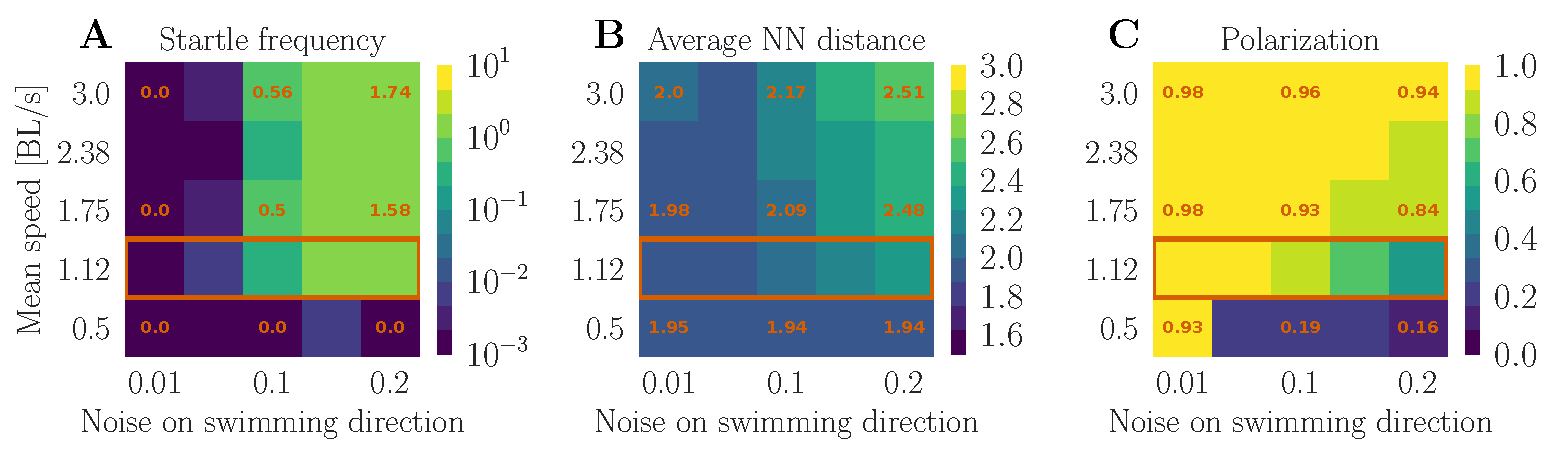
\includegraphics[width=\textwidth]{looming_swarm_fixed_rhonull_int_type_matrix_vis_method_knn_mean_deviate_new.pdf}
    \end{center}
    \caption{\textbf{Startle frequency dependency on collective properties.} Collective behavior results for metric interaction and with KNN-Mean-Deviate as visual integration method (see Section \ref{swarm_methods} for explanation). \textbf{A} Above a mean speed of 0.5 $BL/s$ the startle frequency only depends on the noise on the swimming direction of the individuals. It goes from no startles for very low noise to two startles per second for the highest noise that we analyzed here. \textbf{B} The average Nearest-Neighbor distance increases with noise on the swimming direction similar to the startle frequency but also increases with the mean speed in the range of higher noise values. \textbf{C} The polarization of the collective increases with the mean speed and decreases for higher noise on the swimming direction.}
    \label{fig:swarm_heatmaps}
    \end{figure}
    While we only looked at the mean values over time in Figure \ref{fig:swarm_heatmaps}, in Figure \ref{fig:swarm_over_time} we show how the different measures develop over time.
    For the case with medium direction noise level (left column in Figure \ref{fig:swarm_over_time}) we can clearly see how short periods with many startles affect the polarization as well as cohesion (see e.g. the time point at about 130 s).
    In the right column in Figure \ref{fig:swarm_over_time}, the high direction noise leads to fluctuations of higher amplitude for the polarization and cohesion.
    Additionally, the signals seem to undergo low-frequency oscillations with period lengths of around 60 s to 80 s which we also see for the lower direction noise but less pronounced.\\
    Next, we were interested in the spatial characteristics of single startle events.
    We restricted this analysis to simulations with a mean speed of 1.125 BL/s which is the second row from the bottom in the heatmaps in Figure \ref{fig:swarm_heatmaps}, also indicated by the orange box.
    Unfortunately, the simulations for a direction noise of 0.06 did not result in enough startle events so that we cannot properly analyze the results for this direction noise level.\\
    In the left column of Figure \ref{fig:swarm_startle_stats} we show the position of an agent at the time it startled.
    The coordinate system is build so that the center of mass of the school is at the origin and the mean movement direction of the school points upwards along the y-axis.
    At first glance, the startle positions are distributed similar to the positions of agents that did not startle although the startle positions tend to be more at the center of the school.
    This can be seen more clearly in the right column of Figure \ref{fig:swarm_startle_stats} where we show a histogram of the distance to the center of mass for startles and non-startles.
    Both histograms largely overlap but the startle distances are shifted by a small amount towards the center.
    The direction noise level does not change this pattern.\\
    In the last step of the spatial analysis, we measured the "frontness" of the startling agent by computing the mean movement direction of the group and projecting the position of the startling agent on the vector that originates from the center of mass of the group and points to the mean movement direction.
    The distribution of the frontness values for agents that do not startle (middle column in Figure \ref{fig:swarm_startle_stats}) is symmetric and Gaussian-shaped with the mean value at zero.
    The frontness values of the startling agents have a similar shaped distribution for a direction noise level of 0.1 but the distribution is more narrow which again indicates that the startle positions are closer to the center of the group.
    With increasing direction noise the distribution of startle frontness values becomes more skewed towards positive values, meaning that at high direction noise agents are more likely to startle when they are slightly more in the front than the average agent.\\
    We continue with a comparison of the different methods to determine the visual input of an agent.
    We focused so far on the KMD method where the visual input consists of the difference between the maximal visual angle and the mean of visual angles of the three nearest neighbors (as we fixed k=3).
    If we instead use the mean visual angle of the three nearest neighbors (KMEAN method) as the visual input the most salient difference is an increase of the startling frequency of about one order of magnitude (Figure \ref{fig:swarm_comparison}, left column, first row vs. second row. Note, that we used different colorbar scales in order to make the structure within the heatmaps visible).
    For the KMEAN method we also have startle activity for all combinations of the two parameters mean speed and direction noise which is not the case for the lowest direction noise in the KMD method.
    The effect of the direction noise is here dependent on the mean speed.
    While at higher speeds the startling frequency increases with higher direction noise as we observe it for KMD, at the lowest speed the startling frequency decreases for higher direction noise.
    The overall higher startling frequency is accompanied by nearest-neighbor distances that are up to twice as much as for the KMD method.
    Interestingly, the relationship between startling frequency and average nearest-neighbor distance is reversed for KMEAN because we find the highest nearest-neighbor distance for the lowest startling frequency.
    The polarization follows the same pattern as for KMD with a decrease of polarization for lower speed and for higher direction noise although the polarization does not decrease as much as in the KMD method.\\
    The differences between the MAX and KMD methods are in general similar to those just described for KMEAN.
    The startling frequencies are again much higher and even two to three times as high as for KMEAN.
    In contrast to KMEAN, the startling frequency always increases with increasing mean speed and increasing direction noise.
    Similar to KMEAN, the lowest startling frequency corresponds to the highest mean nearest-neighbor distance but in the case of MAX this point lies at the lowest mean speed and lowest direction noise.
    Finally, the polarization shows the same pattern as for KMD and KMEAN but it does not decrease as much so that the lowest value is at 0.56.    
    \begin{figure}[H]
    \begin{center}
    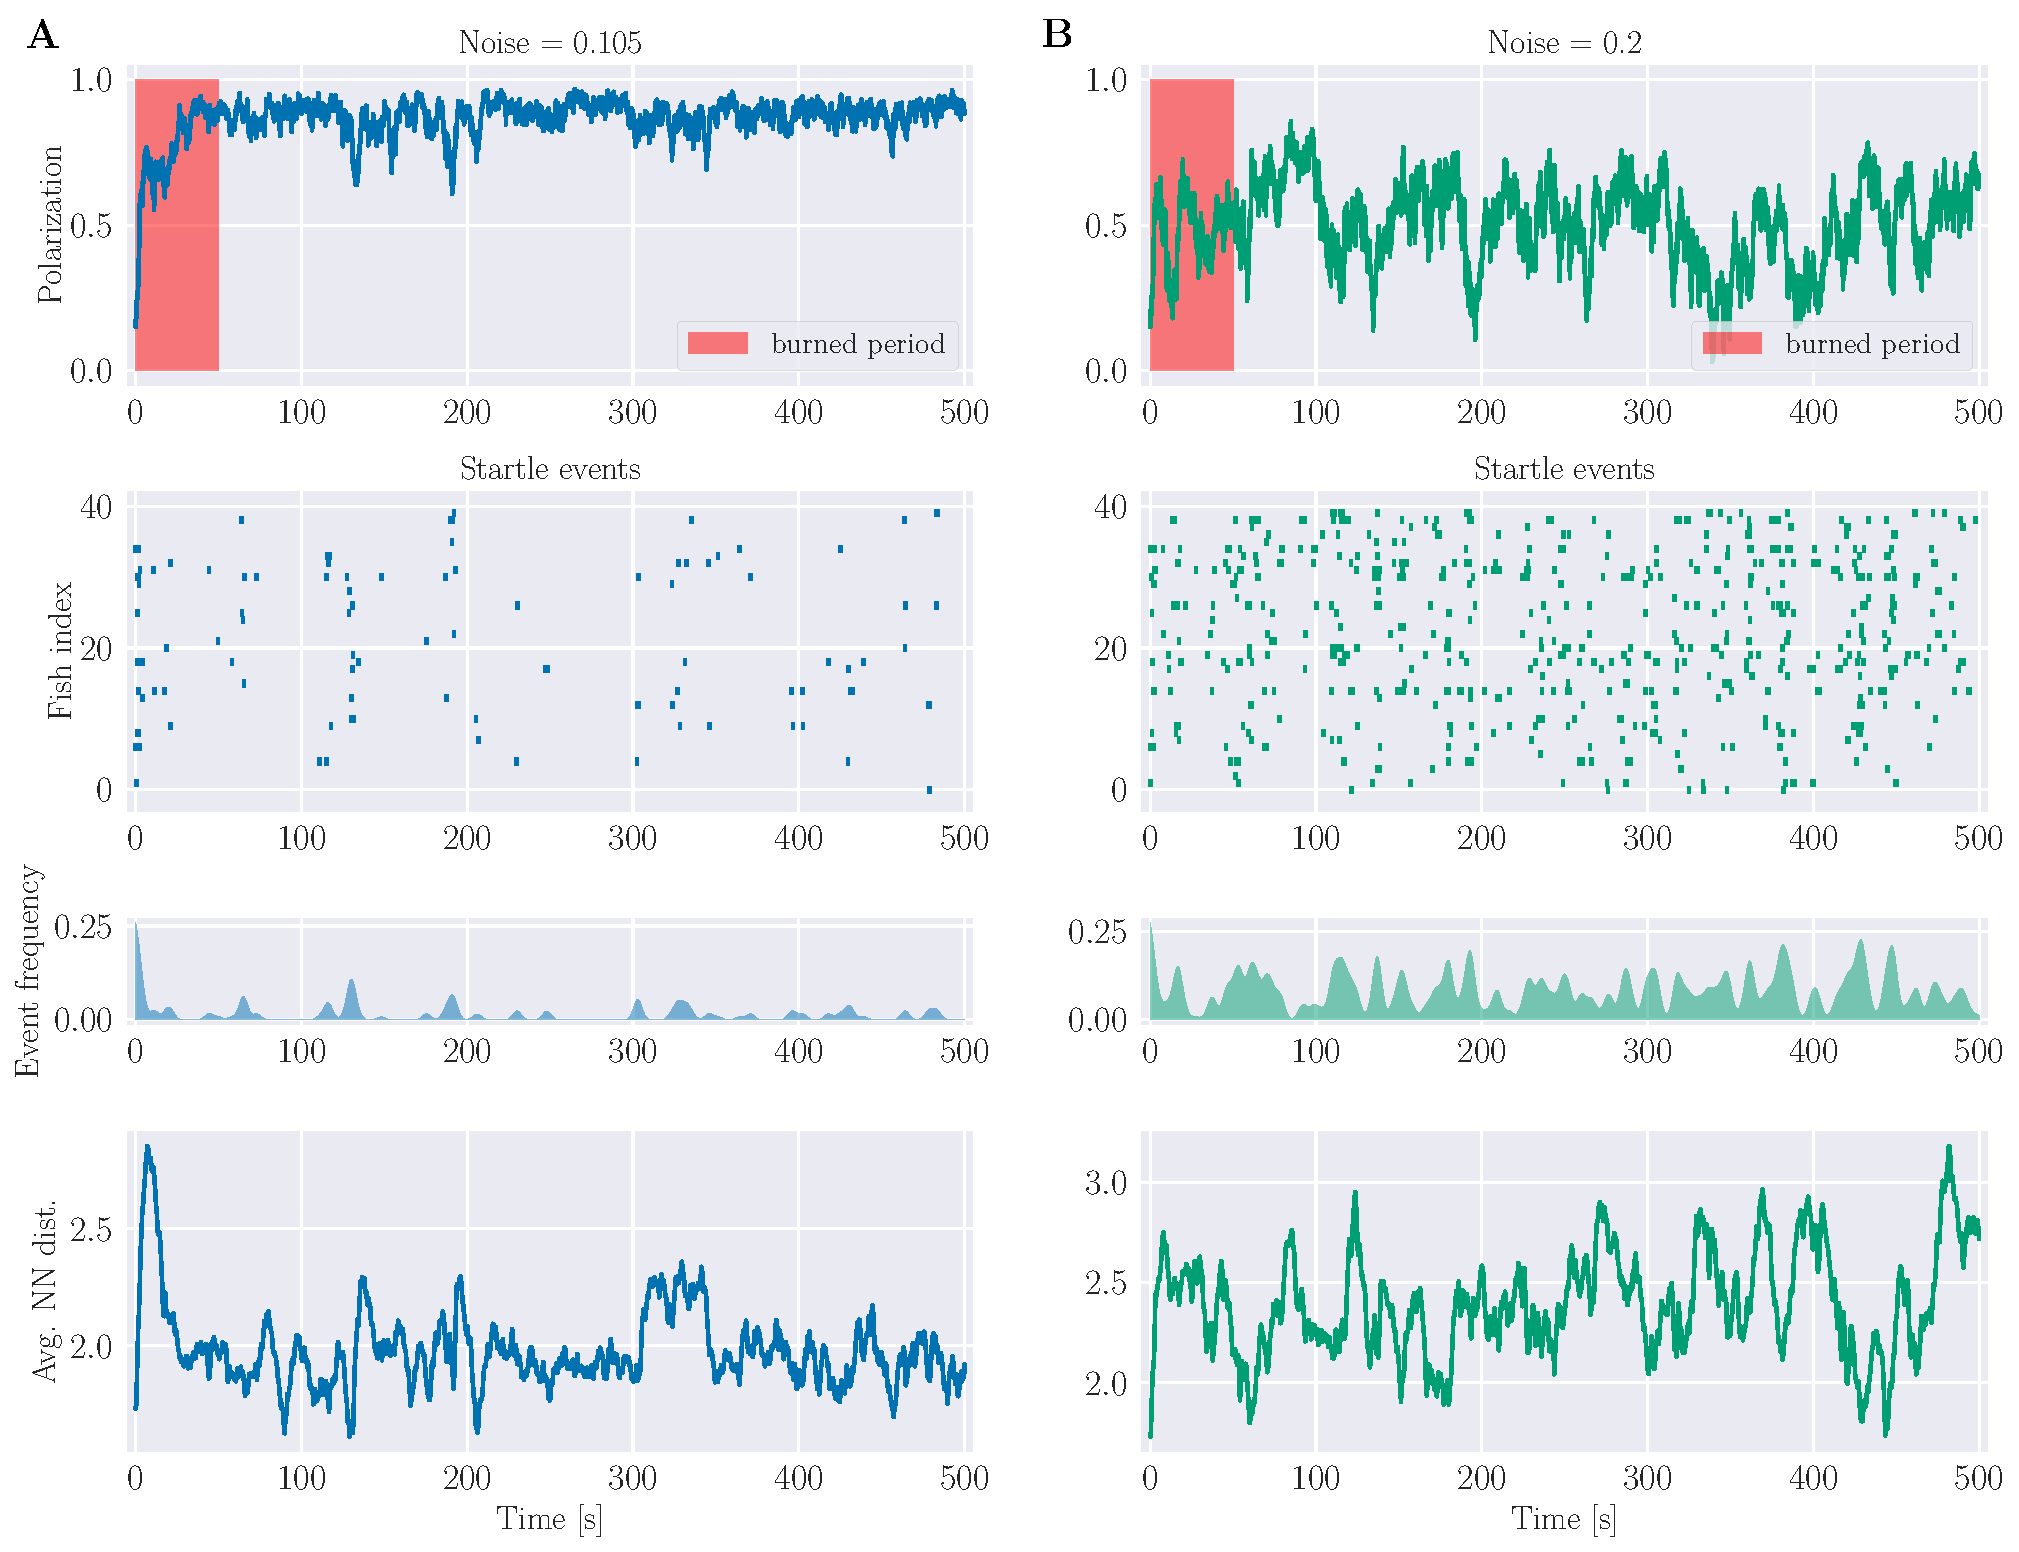
\includegraphics[width=\textwidth]{looming_swarm_over_time.pdf}
    \end{center}
    \caption{\textbf{Collective behavior properties over time for two examples.} The startling frequency, polarization and average nearest-neighbor distance are shown over time from two collective behavior simulations with metric interaction and with KNN-Mean-Deviate as visual integration method (see Section \ref{swarm_methods} for explanation). \textbf{A} For a medium swimming direction noise the polarization (top row) approaches a stable state 50 s after the simulation started. After many startle events in the initial time period the become more rare and come in short waves where many agents startle (second and third row). The group cohesion fluctuates around a value of 2 BL for the average nearest-neighbor distance. \textbf{B} For higher direction noise the polarization of the group shows high amplitude fluctuations around a mean value of 0.5. There are more startle events that seem to occur irregularly over time. The average nearest-neighbor distance shows similar to the polarization bigger fluctuations.}
    \label{fig:swarm_over_time}
    \end{figure}
    
    \begin{figure}[H]
    \begin{center}
    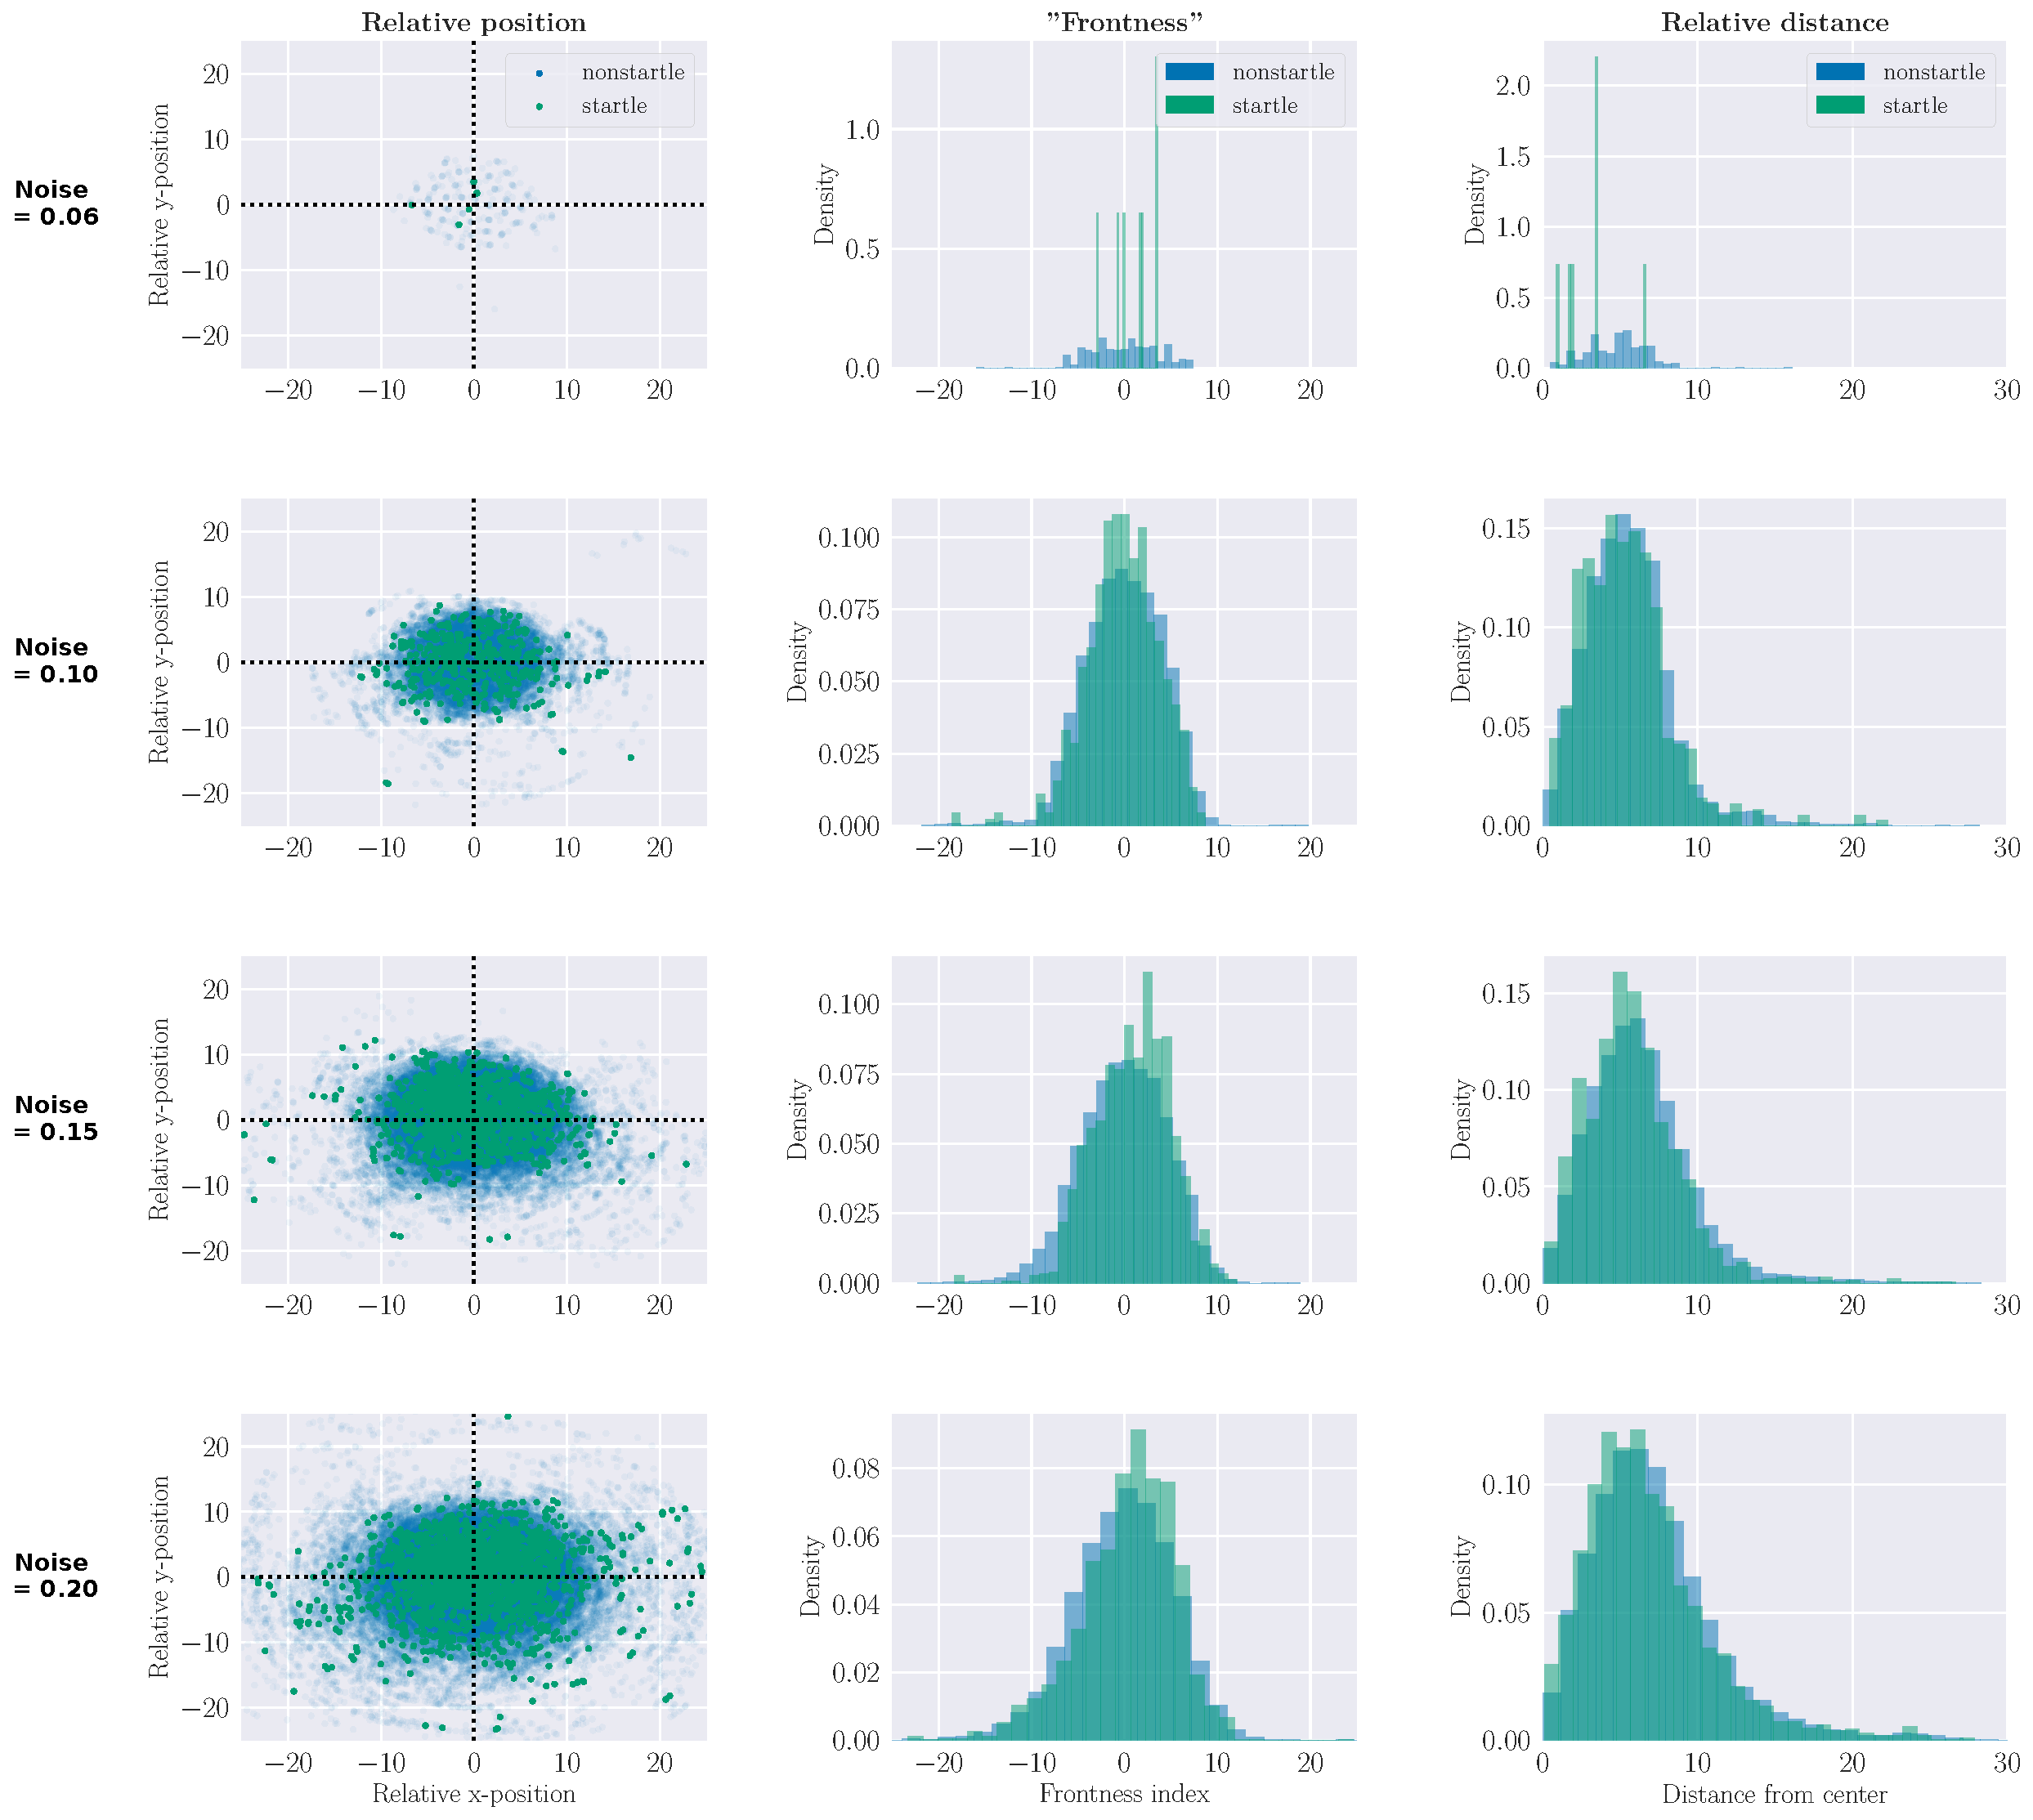
\includegraphics[width=\textwidth]{looming_swarm_startle_stats.pdf}
    \end{center}
    \caption{\textbf{School position at startle events.} Spatial properties of startle events for metric interaction and with KNN-Mean-Deviate as visual integration method (see Section \ref{swarm_methods} for explanation). Each row corresponds to a different direction noise value, starting with the smallest value for which the startle frequency was not zero at the top. The first columns shows for each startle event the relative position of the startling agent (green) and of all other agents (blue). The origin of the plot corresponds to the center of mass of the group and the mean direction in which the group is swimming is upwards along the y-axis. The second column shows the distribution of "frontness" values which is the the projection onto the vector that starts at the center of mass and points in the mean swimming direction of the school. The third column shows the distribution of the euclidean distance to the center of mass.}
    \label{fig:swarm_startle_stats}
    \end{figure}
    
    \begin{figure}[H]
    \begin{center}
    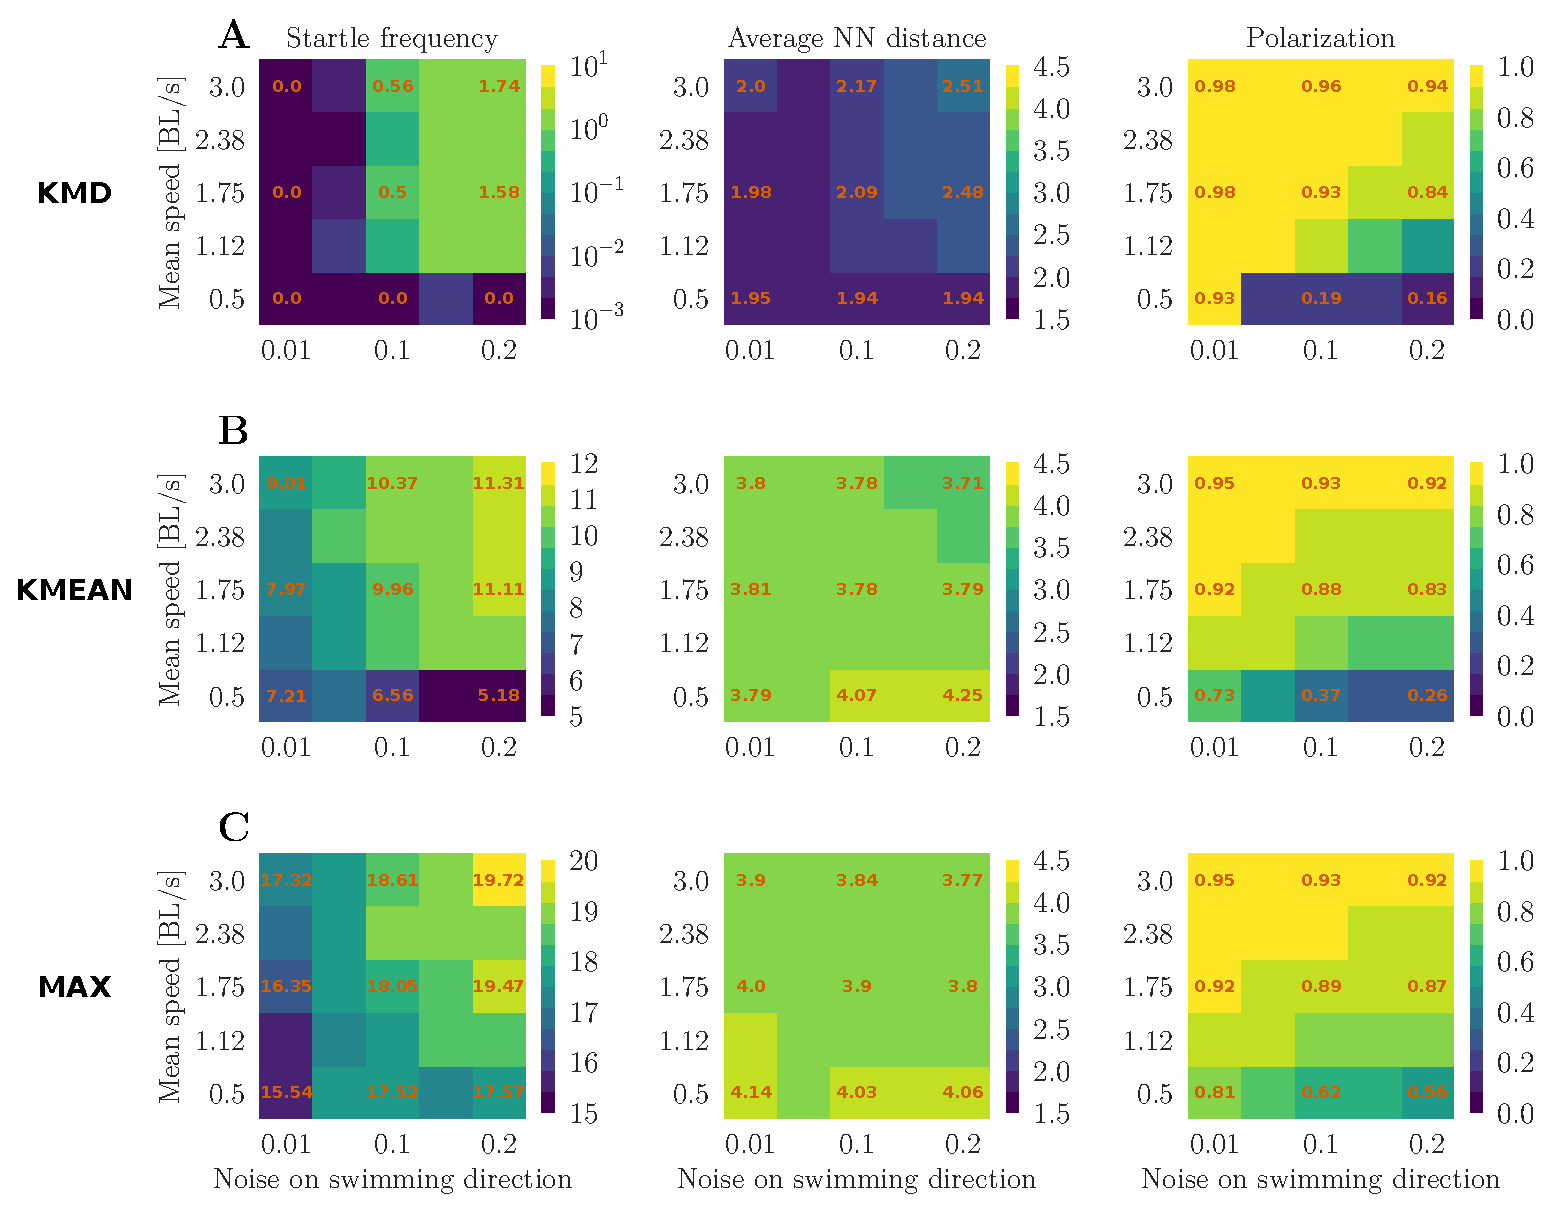
\includegraphics[width=\textwidth]{looming_swarm_fixed_rhonull_int_type_matrix_comparison_new.pdf}
    \end{center}
    \caption{\textbf{Comparison of different visual input methods.} Collective behavior results for metric interaction and different visual integration methods (see Section \ref{swarm_methods} for explanation). The same measurements as in Figure \ref{fig:swarm_heatmaps} are shown. \textbf{A} The same heatmaps as in Figure \ref{fig:swarm_heatmaps}, shown again here for better comparison. \textbf{B} The startle frequency, cohesion and polarization for the KMEAN method. The general patterns with respect to effects of mean speed and direction noise are similar to KMD although the startling frequency is much higher and the average nearest-neighbor distance is almost twice as big. \textbf{C} As for KMEAN, the general pattern is similar to KMD although the startling frequency is much higher for the MAX method.}
    \label{fig:swarm_comparison}
    \end{figure}

\chapter{Discussion}
    In the previous chapter, we presented a model for collective behavior that we coupled with the neuronal model that we fitted in chapter 3.
    We characterized the simulated behavior of the fish school by the startling frequency, cohesion and polarization and how these properties changed with differences in the mean speed of the agents and the noise on the swimming direction.
    This was followed by an analysis of the spatial position within the group that startling agents had at the time of startle initiation and finally we compared the results of different methods for the computation of visual input.\\
    The first effect that we found was that the direction noise strongly increases the startling frequency (Figures \ref{fig:swarm_heatmaps} and \ref{fig:swarm_comparison}).
    We expected this because higher noise makes it more likely that two agents get onto a collision course which resembles the looming stimulus situation and where the visual angle increases quickly enough to evoke the startle response in either or both agents.
    There was one exception, in the case of the KMEAN method and at the lowest speed the startling frequency is highest when the direction noise is lowest (Figure \ref{fig:swarm_comparison} B, bottom row of the heatmap).
    One reason for this exception might be that the agents are not very mobile in this parameter regime, meaning that they change their direction so often that they are mostly staying in one place and thus do not encounter many other agents.
    This is supported by the low polarization and the high nearest-neighbor distance.
    Now the question is why this is not the case for the MAX method and here, the explanation might be that because in the MAX method one close neighbor is enough to evoke the startle response while the KMEAN method requires three close neighbors at the same time.
    Further analysis is needed to answer this question.\\
    Next, we also saw an increase of the startling frequency at higher speeds which is again plausible because more collisions can happen and the social forces might be too slow to change the trajectories of two agents on a collision course which would not be the case at slower speeds.
    This effect hold for all visual input methods that we tested here.\\
    If we look at the relationship between the startling frequency and the two order measures cohesion and polarization it appears that higher startle frequencies go together with higher nearest-neighbor distances but we can not tell from the current analysis if this is a causal relationship.
    It will probably be necessary to analyze the precise sequence of events during each simulation in order to reveal a causal structure.
    Here, it might also be interesting to see, first if there really is a periodicity as we observed it in Figure \ref{fig:swarm_over_time} and second if this can tell us something about the interaction between startling frequency, cohesion and polarization.\\
    If we look at the absolute values of the startle frequency we can say that for this parameter regime the model with the KMD method is the most realistic because its startle frequencies are the only ones that come close to those found in experiments (see beginning of the previous chapter.
    With regards to the experiment from \cite{Rosenthal2015} there are more results that we can compare with our collective behavior model.
    First, we could analyze startling cascades and compare the distribution of sizes with those in the experiment.
    Furthermore, we could check if also in our model the cascade size correlates with the local clustering coefficient.\\
    There are several ways to make the model more realistic.
    One obvious way is to use a more realistic neuronal model for which we already discussed potential extensions in chapter 3.
    For the collective behavior model itself, one assumption that is very likely to not be true in nature is that of the sphere shape of our agents.
    The fact that \cite{Rosenthal2015} found that the subtended visual angle is an important factor for the influence that a startling agent has on its neighbors indicates that it might be important to consider the elongated shape of fish in our model.
    Another promising extension would be to consider computations of the visual input that are based on the actual visual scene.
    Here we took a shortcut by assuming the visual angles of the neighboring agents were already computed somehow and we only analyzed how to combine them.
    Finally, it has been shown that the individuals differ in there decision-making behavior based on their social status \citep{Miller2017} and there are further trait differences in zebrafish \citep{Khan2017}.
    This could be implemented on the neuronal level via different resting activity levels of the inhibitory population.\\
    In conclusion, we developed a biologically motivated neuronal model that can reproduce experimental behavior.
    We coupled the neuronal model with a collective behavior model and found a parameter regime in which the startle frequency is similar to frequencies that were found in experiments.
    But for both models, many possible extensions exist and therefore many open questions remain to be answered.

 

%----------------------------------------------------------------------------------------
%	THESIS CONTENT - APPENDICES
%----------------------------------------------------------------------------------------

%\appendix % Cue to tell LaTeX that the following "chapters" are Appendices

% Include the appendices of the thesis as separate files from the Appendices folder
% Uncomment the lines as you write the Appendices

%\include{Appendices/AppendixA}
%\include{Appendices/AppendixB}
%\include{Appendices/AppendixC}

%----------------------------------------------------------------------------------------
%	BIBLIOGRAPHY
%----------------------------------------------------------------------------------------

\printbibliography[heading=bibintoc]

%----------------------------------------------------------------------------------------

\end{document}  